%% Thesis 1.0
%% "Main Program"
%% 5/10/96 Rich Townsend

%% This is the main program which affects the overall
%% layout of the thesis, and patches all of the
%% chapters together

%% Set up the document class (hacked report)
%% One sided
\documentclass[11pt, a4paper, oneside, openright, fleqn]{thesis}
%% Two sided
%\documentclass[11pt, a4paper, twoside, openright, fleqn]{thesis}

%%%%%%%%%%%%%%%%%%%%%%%%%%%%%%%%%%%%%%%%%%%%%%%%%%%%%%%%%%
%% Package loading stuff
%%%%%%%%%%%%%%%%%%%%%%%%%%%%%%%%%%%%%%%%%%%%%%%%%%%%%%%%%%

% Load in srcltx package for xdvi link
%\usepackage{srcltx}
% NEEDS TO BE REMOVED BEFORE PRINTING!!!!
\usepackage[inactive]{srcltx}

\usepackage[dvipsnames]{color}

% Load in UCL logo package
%\usepackage{uclogo}

% Load in url package
\usepackage{url}

% Load in the xspace package
\usepackage{xspace}

% For adding footnotes to tables
\usepackage{threeparttable}

% For adding colour to tables
\usepackage{colortbl}

% For adding colour to tables
\usepackage[table]{xcolor}

% Load in the ifpdf package
\usepackage{ifpdf}

% Load in the epsf packages
\usepackage{enumerate}

% Load in subcaption package
\usepackage{subcaption} 

% Load in the epsf packages
\usepackage{epsf}

% Load in the epsfig packages
\usepackage{epsfig}

% Load in the calc package
\usepackage{calc}

% Load in Landscape package
\usepackage{lscape}

% Load in Longtable package
\usepackage{longtable}

% Load in Setspace package
\usepackage{setspace}

% Load in the Supertabular package
\usepackage{supertabular}

% Load in the Tabularx package
\usepackage{tabularx}

% Load in the Multirow package
\usepackage{multirow}

% Load in Curves package
\usepackage{curves}

% Load in Epic package
\usepackage{epic}

% Load in the rotating package
\usepackage{rotating}

% Load in the FancyHeadings package
\usepackage{fancyheadings}

% Load in the Afterpage package
\usepackage{afterpage}

% Load in the ifthen package
\usepackage{ifthen}

% Load in the harvard bib style package, and configure it
%\usepackage[abbr]{harvard}
%\citationstyle{apsr}
%\renewcommand{\harvardand}{\&}
%\newcommand{\natexlab}[1]{#1}

% Load in the AmsTeX packages
\usepackage{amsmath}
\usepackage{amssymb}

% Load in the caption
\usepackage{caption}

%ANTONIA PACKAGES
\usepackage{booktabs}

\usepackage{bm}

\usepackage{tabulary}
% Load in the hacked caption stuff
\usepackage{hackcaption}

% Load in PDF hyper link package
\usepackage{hyperref}

% % PDF hyperlinks, with coloured links 
% % (watch for {\it ...} usage - swap to \textit{...})
% \usepackage[pdftex,bookmarks,colorlinks,breaklinks,backref]{hyperref}
% \hypersetup{linkcolor=red,citecolor=blue} % coloured links
% %\hypersetup{linkcolor=black,citecolor=black} % black links, for printed output

% Load in Natbib package
\usepackage{natbib}
\newcommand{\harvardand}{\&}
% Defining the citation style of a given bib style:
% Use \bibpunct (in the preamble only) with 6 mandatory arguments:
%    1. opening bracket for citation
%    2. closing bracket
%    3. citation separator (for multiple citations in one \cite)
%    4. the letter n for numerical styles, s for superscripts
%        else anything for author-year
%    5. punctuation between authors and date
%    6. punctuation between years (or numbers) when common authors missing
% One optional argument is the character coming before post-notes. It
%   appears in square braces before all other arguments. May be left off.
% Example (and default) \bibpunct[, ]{(}{)}{;}{a}{,}{,}
\bibpunct[ ]{(}{)}{;}{a}{}{,}


%%%%%%%%%%%%%%%%%%%%%%%%%%%%%%%%%%%%%%%%%%%%%%%%%%%%%%%%%%
% Page style stuff
%%%%%%%%%%%%%%%%%%%%%%%%%%%%%%%%%%%%%%%%%%%%%%%%%%%%%%%%%%

% Set up the text width and margins in terms of the binding and outer
% margin lengths - here assigned the values dictated by UCL regulations
\newlength{\bindingmargin}
\newlength{\outermargin}
\setlength{\bindingmargin}{40mm}
\setlength{\outermargin}{20mm}


% Work out the text width from these margins and the page size
\setlength{\textwidth}{\paperwidth-\outermargin-\bindingmargin}


% Now work out the LaTeX oddside and evenside margins, taking into
% account the automatic 1in offset which is included.
\setlength{\oddsidemargin}{\bindingmargin-1in}
\setlength{\evensidemargin}{\paperwidth-\textwidth-\bindingmargin-1in}


% Set up all of the other page style stuff
\setlength{\textheight}{235mm}
\setlength{\topmargin}{-0.25in}            
\setlength{\headheight}{7mm}           
\setlength{\headsep}{8mm}              
\setlength{\footnotesep}{1.5ex}
\setlength{\textfloatsep}{14pt plus 6pt minus 2pt}
\renewcommand{\baselinestretch}{1.5}

%% F SIDOLI 2009-05-11
%% Standard empty clear page
\newcommand{\clearemptydoublepage}{\newpage\thispagestyle{empty}\cleardoublepage}
%% Redefined empty clear page to include blank page comment
\newcommand{\clearthesisemptydoublepage}
{\newpage\thispagestyle{headings}\clearthesisdoublepage}

\pagestyle{headings}
%% To add my personal footer to each page comment out line above
%% and uncomment the line below
%\pagestyle{thesis}

\newcommand{\longpage}{\enlargethispage{\baselineskip}}
\newcommand{\shortpage}{\enlargethispage{-\baselineskip}}
\newcommand{\longpagef}{\enlargethispage*{\baselineskip}}
\newcommand{\shortpagef}{\enlargethispage*{-\baselineskip}}
\newcommand{\rb}[1]{\raisebox{1.6ex}[0pt]{#1}}
%%%%%%%%%%%%%%%%%%%%%%%%%%%%%%%%%%%%%%%%%%%%%%%%%%%%%%%%%%

% Font diddles

% Map in the missing math times fonts (this prevents a warning -
% it doesn't do anything useful! )

\DeclareFontFamily{OMS}{ptm}{}
\DeclareFontShape{OMS}{ptm}{m}{n}{ <-> sub * cmsy/m/n }{}

%%%%%%%%%%%%%%%%%%%%%%%%%%%%%%%%%%%%%%%%%%%%%%%%%%%%%%%%%%

% Load in the defs
\typeout{Loading defs....}
\input{defs}


% See if there are any includeonlys
%\typein[\inclist]{Enter includeonly...}
%\ifthenelse{\equal{}{\inclist}}{}{\includeonly{\inclist}}


%%%%%%%%%%%%%%%%%%%%%%%%%%%%%%%%%%%%%%%%%%%%%%%%%%%%%%%%%%%
% Document Start
%%%%%%%%%%%%%%%%%%%%%%%%%%%%%%%%%%%%%%%%%%%%%%%%%%%%%%%%%%%

% If you want to compile one chapter at a time
% but keep the numbering sorted. Must appear 
% before '\begin{document}'

% \includeonly{chapters/chapter1/chapter1}

%%%

\begin{document}

%%---------------------------------------------------------
%% Frontmatter
%%---------------------------------------------------------

%% Do the title page: Personal info for title page
\university{ University College London}
%\faculty{%\Large Faculty of Mathematics and Physical Sciences 
%fa}
\department{Department of Physics \& Astronomy}  
\thesistitle{Dust-Affected Models of Characteristic Line Emission in Supernovae}
\thesisauthor{\huge Antonia Bevan \vspace{0.8cm}}
\dedication{\it{In loving memory of Molly and Bill Siddle.}} 
%\supervisorone{Prof. Michael J. Barlow}
%\examinerone{Dr Kenneth Wood}
%\supervisortwo{Dr Jeremy A. Yates}
%\examinertwo{Prof. Ian D. Howarth}

\maketitle 

%\thispagestyle{empty}

\vspace*{3cm}

\begin{flushright}
\textit{\Large In loving memory of Molly and Bill Siddle.}
\end{flushright}

%% Declaration - REQUIRES SIGNING
\thispagestyle{empty}

\vspace*{3cm}

\begin{flushleft}
I, Antonia Bevan, confirm that the work presented in this thesis is my own. Where
information has been derived from other sources, I confirm that this has been indicated in
the thesis.
\end{flushleft}
%\clearemptydoublepage

%% Abstract
\thispagestyle{empty}
\begin{raggedleft}
\vspace*{23mm}
\hfill {\huge {\bf {Abstract}}} \\
\vspace{6mm}
\hfill \rule{4in}{.015in} \\
\vspace{19mm}
\end{raggedleft}

\noindent{Galaxies and quasars in the very early universe harbour considerable masses of dust, the source of which has been much contested.  For many years it was thought that core-collapse supernovae, though known to form small masses of dust via analyses of dust emission in the infra-red, could not account for the large quantities of dust seen in the early universe.  In recent years, however, this opinion has been challenged by the discovery of reservoirs of cool dust in a number of supernovae containing as much as 1M$_{\odot}$ of dust.  
The late time optical and near-IR line profiles of many core-collapse supernovae exhibit a red-blue asymmetry as a result of greater extinction by internal dust of radiation emitted from the receding parts of the supernova ejecta.  In this thesis, I present  a new code, {\sc damocles}, that models the effects of dust on the line profiles of core-collapse supernovae in order to determine the masses of newly formed dust that form in the ejecta.  The Monte Carlo code and the physical processes therein are described in detail and the testing of the code is presented.  Theoretical profiles are produced in order to understand the effects of varying the parameters of interest on the shapes of the modelled line profiles produced and I discuss a number of other signatures of dust extinction on line profiles aside from the expected blue-shifting.
{\sc damocles} was used to model four different supernovae and supernova remnants.  SN~1987A is a crucial object in the study of core--collapse supernovae and I first present a detailed investigation into the rate of dust formation in this object by modelling the evolution of the H$\alpha$ and [O~{\sc i}]$\lambda\lambda$6300,6363~\AA\ lines.  I also present models of the hydrogen and oxygen lines at late times from SN~1980K, SN~1993J and Cassiopeia A,  all of which display strong blue-shifted asymmetries.
I find that large dust masses are required to fit the late-time line profiles of all of these objects and conclude that core-collapse supernovae are likely an important source of dust in the universe.}





%% Acknowledgements
\thispagestyle{empty}
\begin{raggedleft}
\vspace*{23mm}
\hfill {\huge {\bf {Acknowledgements}}} \\
\vspace{6mm}
\hfill \rule{4in}{.015in} \\
\vspace{19mm}
\end{raggedleft}


\noindent{There are so many people that I want to thank for their help and support. You all, I hope, know who you are. But the last three years have been eventful.  Anyone reading this will probably understand what it means when I say that the writing of this thesis has been among the lesser challenges that I have faced during my PhD.  And so, there are just a few, very heartfelt and uncharacteristically emotional thanks that I wish to make.}

First and foremost, to Mike;  you have been endlessly patient and have always been generous with your time and advice.  You granted me the freedom and space to find my own path through my PhD and I am exceptionally grateful for this.  You have gone above and beyond, especially in difficult times, and I truly thank you.

To Jeremy; your support over the last three years has been invaluable. You have always understood who I was and have guided me carefully and consciously and without preconceptions.    Your encouragement always came at the right times.  

To Patrick; simply put, this thesis would not exist without you!  Thank you for everything; for advice on science and on life, for gossipy drinks and endless cups of tea, for giggling from the start to the end, for your patient understanding and for tea gin. 

To 
Benedict,
Dom,
Fiona,
Georgia,
George,
Jack,
and 
Mike;  my luck in counting you as my friends is beyond words.  I know that every one of you would be there if I needed you, and you have all proved this on numerous occasions over the last three years.  My life is so much the better for having the conversation, laughter and wisdom that you all bring to it.

To Alex;  over the last three years I have watched you become a man, and one of the best.  I could not be prouder to call you my brother.  Knowing that you are always there for me, regardless of circumstance, means more to me than I can say. 

To Nick;  you are my rock. You have been there for me in my darkest moments and my best.  I cannot imagine having done this without you, and I have so many memories that I will cherish for the rest of my life.  You got me through this, as you get me through so much of my life, and I am ever grateful.

To Mum and Dad;  you have been, are, and will always be my best friends in the world.  Support does not even begin to cover what you have given me, not just over the last three years but my whole life.  You are both caring, generous and wise, and I am so lucky to be able to call you Mum and Dad.  I love you.   



%%%%%%%%%%%%%%%%%%%%%%%%%%%%%%%%%%%%%%%%%%%%%%%%%%%%%%%%%%%%%%%%%%%%%%%%%%%
% If you have more than one page in your acknowledgements, include the
% following on each page after the first:
%
% \thispagestyle{fancyplain}
% \lhead[\fancyplain{}{\vspace{4mm}\thepage \vspace{0mm}}]{}
% \rhead[]{\fancyplain{}{\vspace{4mm}\thepage \vspace{0mm}}}
% \cfoot{}
%
%%%%%%%%%%%%%%%%%%%%%%%%%%%%%%%%%%%%%%%%%%%%%%%%%%%%%%%%%%%%%%%%%%%%%%%%%%%



%% Front quote
\thispagestyle{empty}
\vspace*{\fill}

\begin{flushright}
\large {\em QUOTE GOES HERE }\\

\ \

\normalsize
{AUTHOR OF QUOTE GOES HERE}  
\end{flushright}


\vspace*{\fill}
\vspace*{\fill}


\vspace*{\fill}

\vspace*{\fill}

\vspace*{\fill}


%\clearemptydoublepage


%% Contents pages
\addcontentsline{toc}{chapter}{Table of Contents}
\tableofcontents
\clearthesisemptydoublepage
\addcontentsline{toc}{chapter}{List of Figures}
\listoffigures
\addcontentsline{toc}{chapter}{List of Tables}
\listoftables

\addcontentsline{toc}{chapter}{List of Acronyms}


%%List Of Acronyms
\thispagestyle{empty}
\begin{raggedleft}
\vspace*{23mm}
\hfill {\huge {\bf {List of Acronyms}}} \\
\vspace{6mm}
\hfill \rule{4in}{.015in} \\
\vspace{19mm}
\end{raggedleft}




%%%%%%%%%%%%%%%%%%%%%%%%%%%%%%%%%%%%%%%%%%%%%%%%%%%%%%%%%%%%%%%%%%%%%%%%%%%
% If you have more than one page in your acknowledgements, include the
% following on each page after the first:
%
% \thispagestyle{fancyplain}
% \lhead[\fancyplain{}{\vspace{4mm}\thepage \vspace{0mm}}]{}
% \rhead[]{\fancyplain{}{\vspace{4mm}\thepage \vspace{0mm}}}
% \cfoot{}
%
%%%%%%%%%%%%%%%%%%%%%%%%%%%%%%%%%%%%%%%%%%%%%%%%%%%%%%%%%%%%%%%%%%%%%%%%%%%

AAT - Anglo-Australian Telescope

CTIO - Cerro Tololo Inter-American Observatory

HST - Hubble Space Telescope

SED - Spectral Energy Distribution

VLT - Very Large Telescope


%%---------------------------------------------------------
%% Main Body
%%---------------------------------------------------------

% Put your chapters in here


\chapter{Introduction}\label{chp:chp1}

%\begin{flushright}
%  {\em QUOTE GOES HERE }\\
%
%\ \
%
%\normalsize
%{AUTHOR}  
%\end{flushright}


\noindent{Should you choose to seek out one of my friends and ask them about my whereabouts in recent months,
%acquaintances and to enquire of them my whereabouts in recent months
 they would likely stare at you blankly.  Upon further interrogation they would probably yield the information that I was preoccupied writing about dust, a fact which I imagine they  find bemusing and possibly somewhat concerning.  Blissful as they are in their ignorance of dust (astronomers find no such peace), they do not know the importance of this all-pervading substance.}

The universe is an extremely dusty place.  The ubiquity of dust throughout almost all epochs and environments demands a comprehensive understanding of its formation and evolution, properties and effects.  It plays numerous roles in a variety of scenes; it is a building block of  all solid bodies, a birthing place for molecules, a crucial ingredient in star formation and an extreme annoyance for cosmologists.  It is both a product of physical processes and an agent of chemical ones.

It is perhaps confusing therefore that there is comparatively little consensus regarding the formation processes and natal environments that result in the evolution of certain atoms and molecules into the grains we call dust.  Over the years since the first discovery  of dust in the very early universe, a growing population of astronomers and astrophysicists have turned their attention to the study of dust formation in core-collapse supernovae (CCSNe), in the hope that these objects might prove to be the missing piece of the puzzle.  Recent observations of a number of core-collapse supernovae  and remnants have lent weight to this theory, with models and analyses of spectral energy distributions (SEDs)  suggesting the presence of large reservoirs of cool, ejecta-condensed dust. 

I have sought to make my own small contribution to this field by exploiting a different observational signature, that of  blue-shifted line profile asymmetries observed in the spectra of many CCSNe and attributed to the formation of dust in the ejecta.  By quantitatively modelling characteristically asymmetric spectral line profiles using a novel code, DAMOCLES, I have attempted to determine the rate of dust formation in CCSNe and the expected order of magnitude of the eventual dust masses produced.

Throughout the remainder of this chapter I will attempt to elucidate the above synopsis in more detail.  A brief discussion of the roles that dust plays in the universe will be followed by a summary of our current understanding of dust formation in CCSNe.  I will conclude this chapter with a short justification of the approach that I have adopted for this work and an outline of the structure of this thesis.


\section{A Handful of Dust}


\subsection{A Brief History}

The presence of dust in the universe was first theorised when astronomers observed dark patches of sky in the Milky Way where all of the stars had been ``erased" (see Figure \ref{intro:fig:dustpatch}).  Whilst some claimed that these black regions were in fact a true absence of stars resulting from some anomaly in the stellar distribution, others felt that it was more likely that an obscuring cloud of material was blocking the light from the stars behind.  In 1930, Donald \citeauthor{Trumpler1930} confirmed this latter theory by considering the apparent magnitudes and colours of stars located at different angles to the galactic plane, discovering that those closer to the plane appeared redder than their more distant counterparts.  This was the first evidence of interstellar reddening and the beginnings of our understanding of dust as a scatterer, absorber and emitter of radiation.

For the next few decades, dust was thought to be largely an irritating obstacle to observing and comprehending more interesting facets of the universe.  We now have a much fuller understanding of the variety and importance of the roles that dust plays throughout astrophysics.

\begin{figure}
\centering
\includegraphics[scale=0.8]{chapters/chapter1/figs/black_patch_B68.jpg}
\caption{The dark globule Barnard 68, LDN 57.  ESO press release 30 April 1999.}
\label{intro:fig:dustpatch}
\end{figure}

\subsection{The Roles of Dust in the Universe}

Despite comprising only $\sim$1\% of the mass of the interstellar medium (ISM), dust grains account for as much as 30\% of the total galactic luminosity via their emission in the infra-red (IR) \citep{Li2003}.  In the cycle of matter from the ISM to condensing clouds to stars and back again, dust is far more than a passive passenger along for the ride.  Whilst residing in the ISM, dust is important in determining its thermodynamics.  It acts both as a heating agent via the emission of photoelectrons in regions of strong ultra-violet (UV) radiation and a coolant in dense regions via the emission of IR radiation.  In this role as a coolant, dust is also crucial to the process of star-formation, helping to remove gravitational energy and allowing the natal cloud to collapse.  Dust also contributes to the star formation process by shielding the gas from ionising radiation, helping to speed up the construction of the protostellar core. 

In addition to the above physical functions, dust plays an essential part in chemical processes.  Heavy elements in the local medium are depleted through their inclusion in dust grains.  These grains  attract gaseous atoms to their surfaces and catalyse the formation of molecules which are then released back into the surrounding medium.

Dust does not reside solely in the ISM however.  It is present in  large quantities in the circumnuclear tori found around active galactic nuclei.  Dust is also found between planets, around stars and in protoplanetary discs, where dust grains are often the smallest unit of the building blocks that will go on to form planetesimals and planets.  These grains may even be responsible for the origins of life.  

The more detailed our understanding of dust as an astrophysical community, the more accurate we can make our inferences across an entire range of  fields.  There is arguably no other topic in astronomy that has such wide-ranging effects.


\subsection{The Medium of Dust}

An increasingly detailed knowledge of the nature and properties of dust has developed over the last few decades. Dust grains have their terrestrial analogue in soot or very fine sand rather than in the dust bunnies that one may find behind the sofa.  When found in the ISM they are generally small, between 0.05\micron\ and 0.25\micron\ in radius, and are normally predominantly composed of carbon or silicates.  Carbonaceous grains may take many forms ranging from structured solids such as diamond and graphite to amorphous molecules and aromatics.  They are generally found to be strongly attentuating.  Silicates tend to be more glassy and contain silicon and oxygen potentially with the dirtying addition of magnesium, iron or other heavier elements.  Condensates of more complex molecules such as olivine (MgFeSiO$_4$) and pyroxene (MgSiO$_3$) make up these grains.  

Whilst an increasingly strong picture of the composition and properties of dust is becoming apparent, there are still a number of largely unresolved issues regarding the makeup of a dusty medium.
Different species and composites thereof have different optical properties.  In order to model the absorption and scattering of radiation off dust grains it is necessary to first know the complex refractive indices of a given species over the relevant wavelength range.  Laboratory measurements have produced a number of different sets of optical constants for a variety of carbonaceous and silicate species and these are well-utilised throughout the field.  It is noted at this early juncture however that in many cases there are numerous, somewhat contradictory, sets of optical constants for a given species and that these variations can potentially cause a degree of confusion regarding the results of models that utilise them.  This topic will be discussed in detail later in this thesis (SECTION).

Dust grains are generally assumed to be spherical in order to make their simulative treatment more straightforward but in reality dust shapes are actually much more complex.  Sophisticated models of dust grains sometimes adopt a continuous distribution of ellipsoids to represent dust grain shape.  This allows grains to take any ellipsoidal form ranging from flat discs to needles to perfect spheres.  However, even this more detailed consideration omits structures that are akin to long strings or to fluffy particles (not dissimilar to a tumble dryer ball in shape). Heretofore, the vast majority of models, including DAMOCLES, have only considered spherical grains and this wide variety of shapes therefore represents a significant modelling challenge to be addressed in the future.

Dust in the universe follows a cycle.  From its stellar birthplace, it is ejected and slowly integrates itself with the ISM before condensing into molecular clouds and ultimately once again returning to stars.  Most of the knowledge of the properties of dust applies only to grains in the ISM, which are found to follow a grain radius distribution $n(a) \propto a^{-3.5}$ as described by \citeauthor{Mathis1977} in 1977.  This distribution does not necessarily apply immediately after their formation, however, as grains are subject to numerous forces that can result in their destruction, sputtering or evaporation.  The grain size distribution and relative abundances of species of newly-formed grains are still topics in dispute and are issues that I attempt to address in my models.  The issue of dust grain shape will hopefully be addressed in future versions of DAMOCLES.

\section{Core-Collapse Supernovae as Dust Factories}

In an effort to explicate the motivations behind studying dust, I have so far mostly limited my discussion to the evolution and properties of dust after the initial stages of its formation once it has entered the ISM.  The most current and contentious debate, however, is over the natal environment of dust grains.  

Supernovae are the violent explosions that are the death of stars.  They evolve very quickly and create extreme conditions.  Focus on supernovae as a possible source of dust in the universe has been motivated by the physical conditions that they produce shortly after their outbreak and by the presence of large quantities of heavy elements that constitute the integrant ingredients of dust grains.

% are thought to be a possible source of dust in the universe since they produce large quantities of heavy elements and have physical conditions that are potentially suitable for the growth of dust grains.  

\subsection{Types of Supernovae}

Supernovae may be classified into a number of different types.  They are bisected initially into Types I and II according respectively to the absence or presence of hydrogen in their early spectra.  Further sub-classifications depend on  other features in the early spectra, properties of later spectra and the evolution of the  light curve after maximum light.  A summary of the supernova classification scheme is presented in Figure \ref{intro:fig:sn_class}.  

\begin{figure}
\centering
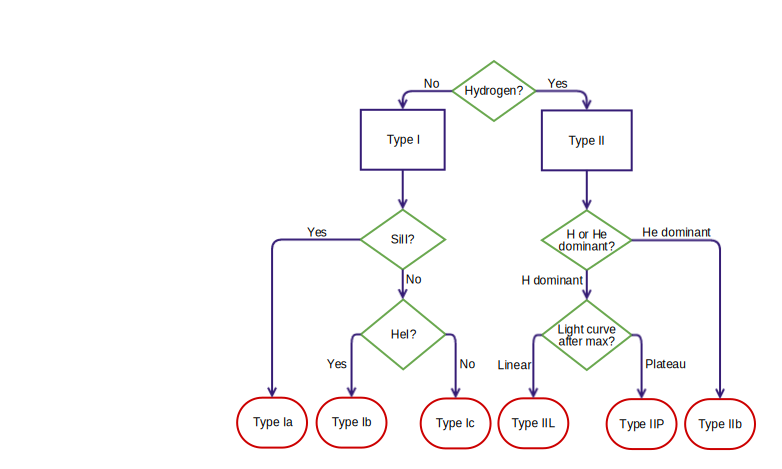
\includegraphics[clip=true, scale = 0.2, trim= 930 50 55 210]{chapters/chapter1/figs/sn_classification.png}
\caption{A flowchart summarising the supernova classification scheme}
\label{intro:fig:sn_class}
\end{figure}

If the initial classification is Type I then all further sub-classifications depend solely on the properties of the early spectra (a few days after explosion) as detailed in Figure \ref{intro:fig:sn_class}.  Type II supernovae are somewhat more complex in their categorisation.  After classification as a Type II, further subdivisions depend on the dominance of hydrogen or helium in \textit{later} spectra.  Helium dominant supernovae are classified as Type IIb and hydrogen dominant supernovae are classified as either Type IIL (those which have a linearly decaying light curve after maximum light) or Type IIP (those that exhibit a plateauing light curve after maximum light).  Type IIn supernovae are omitted from the summary presented in Figure \ref{intro:fig:sn_class} as they cannot be classified straightforwardly via a bifurcating process.  Type IIn supernovae will generally have strong emission lines, particularly hydrogen lines, often with complex profiles.  Crucially, the spectra of Type IIn supernovae do not exhibit the broad absorption features frequently seen in other types and instead contain narrow lines (hence Type IIn).  

\subsection{From Massive Stars to Remnants}

It is generally accepted that the progenitors of Type Ia supernovae are white dwarfs that exist in a binary system with another star.  The accretion of material from one star to another results in a thermonuclear explosion, a mechanism that is unique to Type Ia supernovae.  There have not been any observations suggestive of dust forming in the aftermath of a Type Ia supernova and I therefore do not consider these objects any further, focusing my attention solely on supernovae that explode via the core-collapse mechanism.  

Broadly, this process is initiated when a massive star ($\ge 8$\msun) starts to fuse heavier elements. The fusion of ever heavier elements generates increasingly less energy whilst also causing the mass of the core to increase.  Eventually, radiation pressure drops sufficiently that the core can no longer support itself against its own self-gravity and begins to collapse rapidly. Within milliseconds, the core reaches extremely high densities and, when it can no longer condense further, ``bounces" off itself causing  an immense shockwave to propagate outwards and a vast quantity of energy to be released via the expulsion of neutrinos.  Much of this complex process is still poorly understood and interesting models are currently being produced recreating these very early stages using a numerical approach.  Though the explosion mechanisms of CCSNe are largely beyond the scope of my work, some attention will be paid to these models later in this thesis since instabilities that arise in these early stages can influence the structure of the ejecta at later stages of its evolution.

For several hundred years after the explosion, the supernova (now a remnant) is in the free-expansion phase. During this phase, the mass and velocity of the expanding supernova massively exceed those of the surrounding medium, fortuitously allowing the behaviour of the remnant to be analysed as if it were expanding into a vacuum.  The shock radius during this phase may therefore be calculated simply as $R_s = v_s t$.  As the shockwave propagates through the ISM, interstellar material that has been compressed by the forward shock begins to accumulate.  At the same time a reverse shock wave begins to propagate back through the ejecta.  It is during this phase, which arises very soon after the initial explosion and lasts for a few hundred years, that the physical conditions in the ejecta are thought to be optimal for dust formation.  The phase ends when the mass of material ahead of the forward shock is of a similar magnitude to that behind and the mathematical treatment of its behaviour must be altered.


\subsection{Dust Formation in CCSNe}

Superficially, the formation of dust grains requires densities high enough for interaction between particles to take place, but temperatures that are cool enough to allow the grains to survive.  The theory that the ejecta of a CCSN in its free-expansion phase could provide these conditions  was first hypothesised by \citeauthor{Cernuschi1967} in 1967 and they have now long been thought to be potential dust factories \citep{Hoyle1970, Kozasa1991, Todini2001}.  

The formation of dust was originally thought to result from the stochastic process of classical nucleation whereby particles coalesce to form the seeds of dust grains.  These seeds become the nucleation sites from which grains are ultimately born through the aggregation of further particles.  Various models of dust formation in the ejecta of CCSNe have used this approach \citep{Kozasa1989, Todini2001,Nozawa2003, Schneider2004}.  

More recently, several models of dust formation in CCSNe that consider the effects of chemistry on the growth of dust grains have been published.   These models consider the chemical composition of the gas and include chemical reaction rates thereby considering the manner in which molecular evolution influences dust grain formation and growth rates \citep{Cherchneff2009, Cherchneff2010, Sarangi2013, Sarangi2015}.

Models using both methods have predicted dust masses of the order of 0.1-1\msun of dust forming within the ejecta of CCSNe of progenitor masses between 12-40\msun within the first few years after the initial explosion.

\subsection{The Three Signatures of Dust}
\label{three_sigs}
The presence of dust in the ejecta of CCSNe can be indicated by three main signatures: 

\subsubsection{A decrease in the light curve} 
As the dust begins to form in the ejecta, UV and optical light is absorbed by the dust causing a decrease in the light curve at these wavelengths.

\subsubsection{Excess IR emission}
An increase in emission in the IR occurs contemporaneously with the decrease in the UV-optical light curve.  A thermal MIR excess is caused by warm dust and an excess in the far-IR and sub-mm is the result of cold dust.  The increase in emission in these wavelength can be caused by newly-formed dust condensing in the ejecta but can also be a result of the illumination of pre-existing dust

\subsubsection{Blue-shifted line profiles}
Finally, the onset of the formation of dust can cause an asymmetry in line profiles in the optical and IR.  The absorption and scattering of optical or near-IR radiation by newly-formed dust within the ejecta can result in an asymmetry between the red and blue shifted components, with redwards 
emission from the far side of the ejecta undergoing greater absorption and resulting an overall shift of the profile to the blue.
\\

\noindent All three of these signatures have been discussed in detail over the timeline of this subject but the focus has been on using the excess IR emission seen in the SED of CCSNe to determine quantitatively dust masses in these objects.  This approach has resulted in a lively debate regarding the quantities of dust that CCSNe are capable of producing.
 
\subsection{The Dust Mass Debate}

%%MAYBE MORE DETAIL HERE %%%%
Over the past two decades, several high redshift galaxies  have been found to contain significant masses of dust \citep{Omont2001, Bertoldi2003, Watson2015}.  CCSNe are one of the few potential sources that could contribute large quantities of dust at early epochs. However, 
observations over the last decade at mid-infrared (MIR) wavelengths of 
warm dust emission from CCSNe has suggested that the quantities of ejecta-condensed dust 
produced during the first 1000 days were typically $\leq$ 10$^{-3}$~M$_\odot$  
\citep{Sugerman2006, Meikle2007, Kotak2009, Andrews2010, Fabbri2011}.  This is much less than the 0.1-1.0~M$_\odot$ of dust per CCSN  
estimated to be needed  in order to account for the masses observed \citep{Morgan2003, Dwek2007}.  These observations would indicate that other early-time sources of dust must be found.

 However, recent {\em Herschel} far-IR and sub-mm observations of  several young supernova remnants have revealed cold dust  masses as high as 
0.2-0.8$M_{\odot}$, resulting in a 
re-evaluation of the rate of dust production by CCSNe and a renewed focus on these objects as sources of dust \citep{Barlow2010, 
Matsuura2011, Gomez2012}.

\subsubsection{SN 1987A}


%more waffle on sn1987a

Critical to this field has been the study of SN 1987A.   This supernova is one of the most studied objects in the history of astronomy and has been observed almost continuously since it exploded 28 years ago.  The reason for this is its proximity.  At only ~50pc away, it has allowed for some exceptionally well-resolved spectral and photometric observations.  Neutrinos from its explosion were even detected at three different observatories .  As such, it has yielded results and insight that would not have been possible otherwise and is a key to understanding the formation and evolution of dust in CCSNe.

It is of no surprise therefore that this object has been central to the debate.  \citet{Lucy1989} was the first to suggest the presence of dust in SN~1987A {\em Herschel} observations of SN~1987A were the first to suggest the presence of cold dust in any supernova.



\subsection{Motivation}
%- call something else
It is seems increasingly likely that CCSNe do indeed produce significant quantities of dust.  However, there remain a large number of outstanding challenges to consider.  Firstly, there are still only a very small number of supernovae that have been observed to have sizeable masses of dust present in their ejecta.  If further CCSNe were also shown to have formed large quantities of dust then  the already shifting opinion might start to become consensus.  Other points to consider regarding dust formation and evolution in CCSNe include the nature of the dust (composition, grain size, grain shape etc.) which is still largely unclear, as is the extent to which it is destroyed or sputtered after its initial formation.  Related to this is the uncertainty of the dust formation rate in the ejecta and the issue of where this formation takes place.  These are all interesting questions that call out for answers.  

The {\em Hershel} dust mass estimates were based on fitting dust SEDs that peaked at far-IR wavelengths. Unfortunately, following the end of the {\em Herschel} mission in 2013, there is likely to be a long wait for far-IR facilities with comparable or better sensitivities than {\em Herschel} to become available.  Without data, this methodology is temporarily ineffectual.  This provided an incentive to make use of alternative methods to estimate the dust masses that form in supernova ejecta.

\section{Dust-Affected Line Profiles}

%%MORE HERE

 \citet{Lucy1989} identified a progressive blue-shifting of the [O~{\sc 
i}]~$\lambda$6300,6363~\AA\ doublet from SN~1987A between days 529 and 739 
after outburst, with the doublet in the later spectrum being blue-shifted 
by $\sim 600 $~km~s$^{-1}$. Since then, such red-blue asymmetries have 
been frequently observed in the late-time ($ > 400$ days) spectra of 
supernova ejecta and there is now a growing database of such observations (e.g.
\citet{Lucy1989,Fabbri2011,Mauerhan2012,Milisavljevic2012}).


The purpose of my work has been to develop a new approach to determining dust masses in supernovae, with the aim of providing an alternative to SED fitting for the future and of providing corroborating or contradicting evidence of past results.  I looked to exploit the third signature of dust formation in supernovae, namely the red-clue line asymmetry observed in optical and IR line profiles.  Though this feature has been discussed a length by numerous authors (REFERENCES) it has very rarely been quantitatively measured or modelled.

I have sought to construct a Monte Carlo based code that numerically models this feature in the spectra of SNe in order to quantitatively determine dust masses formed at a variety of epochs post-explosion, additionally seeking to place constraints of the composition and grain size distributions of the newly-formed dust.

\subsection{Observing}

Numerous telescopes have recorded spectra of CCSNe in the optical and IR, some with extremely high resolution.  The Anglo-Australian Telescope (AAT), the Cerro Tololo Inter-American Observatory (CTIO), the Hubble Space Telescope (HST) and the Very Large Telescope (VLT) have all observed several supernovae in the optical including SN 1987A.  Other telescopes such as  the two Gemini Multi-Object Spectrographs (GMOS) have also taken spectra of numerous CCSNe.

Advances in digital storage have allowed for spectral and photometric observations to be made easily available online.  Many observatories now publish their recent observations online in archives and are working to upload observations that pre-date file sharing services.  Much of the data used in this thesis was obtained from these archives. 

\subsection{Modelling}
Need to think about what i actually need to consider in this section.

- dust absorption, scattering and reemission in the IR
- raditaive transfer and independence of optical properties and temp meaning do not need to fully solve rad tran problem
- mie theory deets?  how is it solved and what is the theory?
- assumptions of isotropy?  scattering matrices?
\subsection{Mie Theory}
\label{scn:mie_theory}
In order to truly understand observations that are a product of dust, we must first understand those facets of a dusty medium that determine its interaction with incident radiation.  Dust grain radii are often of a similar order of magnitude to the wavelength of that incident radiation and so may be analysed from an optical perspective using Mie Theory.  Mie Theory is a mathematical solution to Maxwell's equation that describe how light is scattered off a small particle.  In combination with the optical properties of the medium, this allows for a precise determination of the extinction and scattering efficiencies of a given environment.  Conveniently, this allows for the straightforward modelling of a dusty medium and it is this calculation that I exploit in my models.  Mie Theory assumes particles to be spherical, an assumption which is a potential issue since grains may be crystalline, fluffy or extremely amorphous.  This issue is addressed later in this thesis.



\section{Content Of This Thesis}
And relate to your current work - give an overview of the work and what you did as well as the structure of the thesis - see Jo's for example.

%\clearthesisemptydoublepage
\chapter{Details of the Monte Carlo Code}\label{chp:chp2}

%\begin{flushright}
%  {\em QUOTE GOES HERE }\\
%
%\ \
%
%\normalsize
%{AUTHOR}  
%\end{flushright}


\section{Monte Carlo Methods}
	 
	 \noindent{The name 'Monte Carlo' describes a class of modelling techniques that employ a stochastic approach to simulating mathematical and physical situations that are otherwise difficult or impossible to solve.  By repeatedly sampling random numbers from a probability distribution, numerical results to non-analytic problems may be obtained.  The approach was first used by researchers at Los Alamos in the late 1940s who adopted the method to model the transport of neutrons.  It is from the code name for this project, 'Monte Carlo', that the methods derive their name.  }
	 
	 As the available computing power increased over the following decades, Monte Carlo methods became more and more useful as a means of solving complex problems and are now used widely across numerous fields including mathematics, statistics, engineering, finance, the physical sciences and many others.  The nature of the approach means that they are particularly well-suited to problems with multiple degrees of freedom, and especially when any of these degrees are coupled.  By using random numbers to represent quantities that parametrise a physical problem, a model may be generated that simulates a solution to the problem using a pseudo-random number generator.   It must be the case that the quantities that characterize the problem may be represented by a continuous distribution in the range [0,1] in order that randomly generated numbers may be translated into physical properties.  
	 
	 For each randomly-generated input, the model of interest is applied and an output - a 'possible outcome' - is obtained.  By iterating this process many times with randomly-generated inputs each time, many possible outcomes are generated and a probability distribution may be built up.  The interpretation of the outputted probability distribution is dependent on the manner of utilisation of the Monte Carlo method.  For example, the iterative procedure may be used to determine best-fitting parameters of a model or may be used to find the mean-free path of a photon.  In the former case, the multi-dimensional probability distribution may be analysed to determine the most representative model or models whereas in the latter case the probability distribution is equivalent to an energy distribution.
	 
	 Clearly, Monte Carlo simulations are limited by their finite nature and will never produce a perfect solution.  However, this does not mean that Monte Carlo simulations are lacking in rigour.  It may be shown that the error in a Monte Carlo model is approximately $\sim \frac{1}{\sqrt{n}}$ for large $n$, where $n$ is the number of quanta used in the simulation.  The error may therefore be made as small as required by increasing the number of quanta used in the simulation subject to the restrictions of computing time and expense.
	 
	 In the next section, I discuss the use of Monte Carlo methods as applied to radiative transfer problems and  specifically to DAMOCLES.  I discuss the computational aspects of my work and the architecture of the code in section \ref{damocles_struct} before finally discussing the limitations of the code and its potential for future developments in section \ref{limitations}.
	 
\section{Radiative Transfer and the Monte Carlo Method}
\label{rt}

 The application of Monte Carlo codes to radiative transfer problems in astrophysics has a strong history.  Numerous codes that utilise this stochastic methodology have been written in the past few decades in order to model the transport of photon packets through various media.  The energy to be transported throughout the region of interest is discretised into packets and the path of each packet is calculated according to the properties of the environments that it passes through during its lifetime.  Collating the escaped packets at the end of the simulation produces an energy distribution. 

There exist several Monte Carlo radiative transfer codes that use this technique in order to model the transfer of line emission through a nebula to produce a synthetic spectrum. There also exist a number of codes that treat the continuous emission and absorption of energy in dusty environments in order to produce and fit a spectral energy distribution (SED).  Models of supernovae have been produced using both approaches and well-fitting spectra and SEDs have been generated but never, according to the best of my knowledge, has the mechanism been employed to produce sophisticated models of line profiles in expanding dusty regions.  In this new code, we seek to apply the technique to an expanding dusty medium in order to consider the effects on a single emitted line profile.

Previous work by Leon Lucy has considered the problem of dust-induced asymmetric line profiles in the ejecta of supernovae and he has published results derived both analytically and using simple Monte Carlo simulations.  These simulations appear to be the only published instances of a numerical approach to studying this spectral feature.  The DAMOCLES code adopts the same technique as the original modelling by Leon Lucy but allows for a considerably more complex treatment of the composition, geometry and motion of the dusty medium.

Radiative transfer methods as applied to supernovae generally treat a wide wavelength range and seek to conserve the total energy.  In the case of SED modelling, this is often achieved by dividing the total energy into packets of equal weight and energy, and iteratively determining the temperature and ionization structure.  In this work, the approach we adopt is somewhat simpler as only a very narrow wavelength range need be considered.  Rather than seeking to conserve the total energy, we assume that any packet absorbed by dust would be re-emitted outside the wavelength range of interest and thus no longer contributes to the resulting line profile.  Any absorbed packet is therefore removed from circulation.  In addition to this, the absorption and scattering of radiation by dust is independent of temperature and there is therefore no need to calculate temperatures throughout the nebula.  Similarly, in the case of radiative modelling of synthetic spectra of the ejecta of supernovae, approximations such as the Sobolev approximation are often employed to handle the blending of lines more efficiently.  This is unnecessary here as only a single line or doublet is ever treated and a comparatively narrow wavelength range considered. 

The subtleties of the problem we consider here lie in the treatment of an atmosphere expanding as fast as 10\% of the speed of light.  Lorentz transforms must be carefully applied in order that packets experience the appropriate degree of frequency shifting at emission and at each subsequent scattering event.  In this respect, the code is analogous to Monte Carlo radiative transfer models of electron scattering published by \ref{}.  Indeed, similar features are observed in the outputs of both.

Throughout this section, I will describe the principles, assumptions and techniques adopted in the production of the DAMOCLES before I move on to address the mechanics and architecture of the code itself.  DAMOCLES stands for \textbf{D}ust-\textbf{A}ffected \textbf{M}odels \textbf{O}f \textbf{C}haracteristic \textbf{L}ine \textbf{E}mission in \textbf{S}upernovae.
 

	\subsection{Energy Packets}
	
	The fundamental principle underlying the transport of radiation throughout a dusty nebula is that the radiation be discretised into packets.  Each of these packets is then propagated throughout the nebula and ultimately contributes a fraction of the final energy distribution.  At the start of the simulation, each packet is assumed to consist of $n$ photons of frequency $\nu_0$, the rest frequency of the line to be modelled.  All packets therefore begin life with initial energy

\begin{equation}
	E_0=nh\nu_0
\end{equation}
	
	
	where $h$ is Planck's constant.  As the packets move through the ejecta, they are scattered off high-velocity dust grains and after each scattering event, the frequency of the packet is altered.  In Monte Carlo simulations that model non-moving atmospheres, packets are usually taken to be of constant energy.  When the frequency of a packet is altered after an event, the energy of that packet is kept constant and the number of real photons contained within it assumed to change.  However, in the case of dust scattering, the number of real photons is conserved and thus the energy of the packet is altered.  This is most easily achieved by weighting each packet over all scattering events as 
	
\begin{equation}
	w=\prod_{scat} \frac{\nu'}{\nu}
\end{equation}

\noindent where $w$ is the weight of the packet.  The final energy of each packet is then $E =w E_0$, where $E_0$ is the initial energy of the packet.  The final dust-affected line profile is compiled by adding the total energy of all packets in a specific frequency bin in order to produce a histogram.
	
	In these models, unlike fully self-consistent SED radiative transfer models, there is no requirement that the total energy be conserved.  We drop this traditional requirement since radiation that is absorbed by dust is re-emitted outside of the wavelength range of interest and thus no longer contributes any flux to the resulting line profile.  Packets that are absorbed may be safely removed from the simulation.
	
	\subsection{Initialisation and the Grid}
	
	The supernova ejecta is approximated by a three-dimensional cartesian grid, each cell of which is assumed to have uniform density and composition.  By default, the ejecta occupies a shell between inner radius $R_{in}$ and outer radius $R_{out}$. The grid extends from $-R_{out}$ to $+R_{out}$ in each of the three axes.  Each side is split into the same number of divisions and thus each cell is a cube of volume $R_{out}^3/n_{div}^3$ where $n_{div}$ is the number of divisions along each axis and is specified by the user.  For the remainder of this thesis, a spherically symmetric situation is assumed and in all modelling and testing the grid is constructed in this manner.  However, there are no assumptions of symmetry in the code and a cartesian grid was adopted in order to allow for arbitrary geometries to be modelled in the future e.g. ellipsoidal or toroidal ejecta distributions.
	
	  Both gas and dust are by default assumed to have a power-law distribution declared as  $\rho(r) \propto r^{-\beta}$ between $R_{in}$ and $R_{out}$.  The distribution of gas determines the emissivity distribution and thus the starting positions of the packets in the simulation (see section \ref{sctn:em_prop}).  However, after the initial emission of energy packets, the gas plays no further role in the simulation as only interactions with dust grains are of interest here.  By default, the dust is coupled to the gas and thus follows the same smooth power-law distribution previously described with exponent $-\beta$.  The dust density in each cell is therefore calculated as
	
\begin{equation}
\rho (r)= \frac{M_{tot}(3-\beta)}{4\pi (R_{out}^{3-\beta}-R_{in}^{3-\beta})}
\end{equation}
	
	
\noindent where $r$ is the radial distance from the centre of the cell to the origin and $M_{tot}$ is the total desired dust mass to model.  Any cell whose centre falls outside of the bounds of the supernova ejecta has dust density set to zero.  If the dust and gas are decoupled then the user must specify distinct profiles for the gas and the dust; that is, separate power laws must be declared and independent inner and outer radii specified.  This allows for more sophisticated modelling of, for example, circumstellar shells or dense cores of dust formation surrounded by more diffuse gas.

It is known from SED modelling that clumped environments produce very different results to environments assumed to have a smooth distribution of dust and gas.  Generally, in comparison to smooth models, clumped models tend to require more dust in order to reproduce a similar level of emission or absorption.  The capacity for modelling a clumped dusty medium is therefore included in the code.  The fraction of the dust mass that is in clumps is declared ($m_{frac}$) and the total volume filling factor of the clumps ($f$) is also specified.  Dust that is not located in clumps is distributed according to a smooth radial profile.  The clumps occupy  a single grid cell and their size can therefore be varied by altering the number of divisions in the grid.  They are distributed stochastically with probability of a given cell being a clump proportional to the smooth density profile (i.e. $p(r) \propto r^{-\beta}$).  The density of all clumps is constant and is calculated as 

\begin{equation}
\rho_{clump}=\frac{M_{clumps}}{V_{clumps}}=\frac{m_{frac}M_{tot}}{\frac{4}{3} f\pi (R_{out}^{3}-R_{in}^{3} )}
\end{equation}

\noindent where $M_{tot}$ is the total dust mass, $M_{clumps}$ is the total dust mass in clumps and $V_{clumps}$ is the total volume occupied by clumps.  $m_{frac}$ and $f$ are defined as above.
	
A grid of cubic cells of varying dust and gas densities is thus produced in readiness for packets to be transported through it.  A frequency grid is also established centred on the rest-frame frequency of the line to be modelled.

	
	\subsection{Properties of the Dusty Medium}
	Dust of any composition may be used for which optical data is available.  The relative abundances of the species must be declared in an input file accompanied by a grain size distribution for each species.  Files detailing the optical data ($n$ and $k$ values) for the chosen dust species are also declared at the start of the code.  For each frequency and grain size pair, a Mie scattering routine uses this data to calculate the overall $Q_{abs}(\nu)$ and $Q_{sca}(\nu)$ by summing over the weighted grain sizes and species.  This value is then used in the calculation of the opacity of each grid cell, which determines the fate of any packets passing through it.  A Mie scattering routine is an appropriate approximation in this instance as it applies in the case of spherical scatterers where the diameter of the sphere is of the same order as the wavelength of the interacting photon.  The wavelengths of the lines of interest for this code (particularly 6563 \AA \:H$\alpha$ and 6300 \AA \:[OI])  are in the optical and near-IR  and wavelengths are therefore of the order of 0.3-1.0$\mu$m, as are dust grain radii.
%!!!! GO INTO MORE DETAIL ABOUT MIE SCATTERING AND REPHRASE THIS SECTION
	


	\subsection{Emission and Propagation}
	\label{sctn:em_prop}
	The initial radiation field is inherently tied to the distribution of gas throughout the supernova ejecta.  The relationship between the emissivity and the gas density may vary under different regimes and therefore the emissivity distribution is also specified as a power law with $i(\rho) \propto \rho^{k}$.  In general, however, this is taken to be $i(r) \propto r ^{-2\beta}$ since the majority of lines modelled are recombination lines and therefore $i(\rho) \propto \rho^2$.  The supernova ejecta is divided into shells between $R_{in}$ and $R_{out}$ and the number of packets to be emitted in each shell calculated according to the specified distributions.  For each packet a location within the appropriate shell is determined by randomly sampling from an isotropic distribution.  Three random numbers in the range [0,1) are sampled and these are translated into spherical coordinates as 

%\begin{equation}
	\begin{align}
		\phi&=2\pi\eta \\
		\theta&=\arccos(2\xi -1) \\
		r&=R_i+\zeta(R_{i+1}-R_i)
		\label{eqn:isotropic}
	\end{align}
%\end{equation}

\noindent where $\eta$, $\xi$ and $\zeta$ are random numbers, $\phi$ is the azimuthal angle, $\cos \theta$ is the radial direction cosine and $R_i$ is the inner boundary of the $i$\textsuperscript{th} shell.  At emission and at every subsequent scattering event, the packet is propelled with a new direction vector which is sample from an isotropic distribution.  I do not include forward-scattering matrices in the code since the effects of forward scattering by dust are so small as to be negligible and it is simpler and more efficient simply to assume isotropic scattering.  Having calculated an emission location, an initial propagation direction vector $(\theta,\phi)$ must be obtained.  This is calculated in exactly the same manner as described in equation \ref{eqn:isotropic} but for two newly generated random numbers.

Once a packet has been emitted into the nebula, it must be propagated through the grid until it escapes the outer bound of the ejecta $R_{out}$.  If it is not absorbed, its trajectory must be calculated and its weighting updated as it undergoes repeated scatterings.  In each cell that a packet passes through, a test is performed to determine whether the packet passes through that cell and into the next of whether it experiences an event, either scattering or absorption.  I calculate this by considering the probability that the packet travels a distance $l$ without interacting as 

\begin{equation}
p(l)=e ^{-n \sigma_{\nu} l}=e ^{-\tau_{\nu}} 
\end{equation}

\noindent where $n$ is the number density, $\sigma_{\nu}$ is the cross-section of interaction at frequency $\nu$ and 

\begin{equation}
 \tau_{\nu} = n\sigma_{\nu} l = \rho \kappa_{\nu}  l
 \end{equation}
 
 \noindent for constant $n$ and $\sigma_{\nu}$ (as in a grid cell).  The probability that a packet \textit{does} interact within a distance $l$ is therefore $1-e^{-\tau_{\nu}}$.  We may sample from the cumulative probability distribution to give: 

\begin{align}
\xi &= 1 - e^{-\tau_{\nu}}  \\
\implies  \tau_{\nu}&=-\log (1-\xi) 
\end{align}

\noindent where $\xi \in [0,1)$ is a sampled random number equivalent to the value of the optical depth for that packet in that cell.  The frequency of the photon packet and the mass density of the cell are then used to calculate the opacity of that cell and, using the fact that $n\sigma_{\nu}=\kappa_{\nu}\rho$, the distance $l$ that the packet travels before its next interaction is calculated.  If this value is greater than the distance from its position to the edge of the cell then the packet is moved along its current trajectory $(\theta,\phi)$ to the cell boundary and the process is repeated.  Alternatively, if the displacement is not sufficient for the packet to escape the cell then an event occurs.  The packet is either scattered or absorbed with probability of scattering equal to the albedo of the cell

\begin{equation}
	\omega=\frac{\sigma_{sca}}{\sigma_{sca}+\sigma_{abs}}
\end{equation}

If the packet is absorbed then it is simply removed from the simulation as discussed above.  If the packet is scattered then a new trajectory is sampled from an isotropic distribution in the comoving frame of the dust grain and the frequency of the packet recalculated using Lorentz transforms as described in the next section.  This process is repeated until the packet has either escaped the outer bound of the supernova ejecta or been absorbed.  Escaped packets are added to frequency bins weighted by $w$ in order to produce an overall emergent line profile.


	\subsection{Doppler shifting}
	
At emission and at each scattering event the frequency of the packet is recalculated according to a radial velocity field 
	
\begin{equation} 
	v(r) = v_{max}\frac{r^{\alpha}}{R_{out}^{\alpha}}
\end{equation}

\noindent where the maximum velocity, $v_{max}$, at the outer edge of the ejecta and the exponent of the velocity profile, $\alpha$, are declared in the input file.	
		
It is worth noting that if a constant mass loss rate is required, the exponent of the velocity profile and the exponent of the density profile are not independent.  A constant mass loss rate implies that $4\pi \rho vR^2  \propto k$, where $k$ is a constant, and thus for $v \propto r^\alpha$ and $\rho\propto r^{-\beta}$, we require that $\beta-\alpha=2$.  However, it is possible that the supernova event may have induced a mass-flow rate that is not constant with radius and thus both exponents may be declared independently.  It is also worth noting that for supernovae in their free expansion phase, as the majority are by the time of the onset of dust formation, the ejecta are expanding with a $v \propto r$ Hubble law expansion.
	
The outflow velocities in supernovae are extremely high of the order of 10\% of the speed of light.  Escaping radiation is therefore subject to significant, relativistic Doppler shifting. At emission and at each scattering event, the frequency of a packet must be recalculated according to the velocity of the scattering or emitting grain.  When the packet is initially emitted, it has a frequency and a trajectory in the rest frame of the emitter. Both of these must be transformed to the observer's frame in order for the packet to be propagated through the grid.  The new direction and frequency in the observer's frame may be simply found by transforming the momentum 4-vector $\boldsymbol{P}$ which is defined as

\begin{equation}
\boldsymbol{P}=
\begin{pmatrix}
	E \\
	p_x \\
	p_y \\
	p_z \\
	\end{pmatrix} =
	\begin{pmatrix}
	h \nu \\
	h \nu x \\
	h \nu y \\
	h \nu z \\
	\end{pmatrix}
\end{equation}


\noindent We may then derive $\boldsymbol{P'}$, the momentum 4-vector in the observer's frame using the relation

\begin{equation}
	\boldsymbol{P'}=\Lambda \boldsymbol{P}	
\end{equation}

\noindent where 

\begin{equation}
	{\Lambda}=
	 \begin{pmatrix} 
	 \gamma & -\gamma \beta_x & -\gamma \beta_y & -\gamma \beta_z \\
	-\gamma \beta_x & 1+(\gamma-1)\frac{\beta_x^2}{\beta^2} & 
	(\gamma-1)\frac{\beta_x \beta_y}{\beta^2} & (\gamma-1)\frac{\beta_x \beta_z}{\beta^2} \\
	-\gamma \beta_y  & (\gamma-1)\frac{\beta_y \beta_x}{\beta^2} & 1+(\gamma-1)\frac{\beta_y^2}{\beta^2} 
	& (\gamma-1)\frac{\beta_y \beta_z}{\beta^2}\\
	-\gamma \beta_z & (\gamma-1)\frac{\beta_z \beta_x}{\beta^2} & (\gamma-1)\frac{\beta_z \beta_y}{\beta^2} 
	& 1+(\gamma-1)\frac{\beta_z^2}{\beta^2} \\
	 \end{pmatrix}
	 \\
\end{equation}
\\
\\
 \noindent and $\boldsymbol{\beta}=\frac{{\bf{v}}}{c}$,   $\boldsymbol{\beta}=(\beta_x,\beta_y,\beta_z)$,   $\beta=\lvert \boldsymbol{\beta}\rvert$ and $\gamma = \frac{1}{\sqrt{1-\beta^2}}$.
 \\

In practice, the velocities considered are low enough that it is unnecessary to consider terms of order $O(\frac{v^2}{c^2})$ and thus ${\Lambda}$ may be reduced to

\begin{equation}
	{\Lambda}=
	 \begin{pmatrix} 
	 1 & - \beta_x & - \beta_y & - \beta_z \\
	- \beta_x & 1 & 0 & 0 \\
	- \beta_y  & 0 & 1 & 0\\
	- \beta_z & 0 & 0 & 1 \\
	 \end{pmatrix}
	 \\
\end{equation}

\noindent The new direction of travel and frequency in the observer's frame are therefore given by  
\begin{equation}
\nu'=\nu(1-x\beta_x-y\beta_y-z\beta_z) \\
\end{equation}
\begin{equation*}
\begin{split}
x'=\frac{\nu}{\nu'}(x-\beta_x) \\
y'=\frac{\nu}{\nu'}(x-\beta_y) \\
z'=\frac{\nu}{\nu'}(x-\beta_z) \\
\end{split}
\end{equation*}

For each scattering event, the packet must be transformed both into and out of the comoving frame. The reverse transform is applied by using the inverse Lorentz matrix $\Lambda^{-1}$ which is obtained by reversing the sign of $\bf{v}$.  Positive $\bf{v}$ is defined for frames moving away from each other and thus $\bf{v}$ is defined to be negative in the direction of the observer.
	

	\subsection{Electron Scattering}
	As will be discussed in detail in chapter three, the effects of scattering on the shapes of line profiles can potentially be quite pronounced and it is therefore important to consider the potential effects of electron scattering as well as those of dust scattering.  A simple treatment of electron scattering calculates electron densities using an estimated average temperature of either 5000K, 10,000K or 20,000K.  An observed luminosity of $H_{\alpha}$ is then used to calculate the optical depth to electrons.  Electron scattering is treated in an identical manner to dust scattering with the overall optical depth $\tau = \tau_{dust}+\tau_{e}$ in each cell.  If, for a given packet, an event ocurrs, it is first calculated whether this is a dust event or an electron scattering event by considering the ratio of the optical depths of each species to the total optical depth.  If the packet is scattered by an electron then this process is identical to dust, but the velocity of the scatterer now has a thermal component that must be considered.  
	
	%ES CALCN HERE.

In the majority of cases it seems that the electron densities are not high enough to discernibly effect the overall shape of the profile.  However, there may be a few rare cases (the concept is discussed for SN 2010jl \citep{Fransson2013}) where the electron densities are high enough to become significant in the observed profiles.  Whilst the inclusion of electron scattering in the code is an approximation, it gives a good suggestion of the potential effects of electron scattering.	
	
	\subsection{Doublets}

One of the lines in supernovae emission spectra that is frequently seen to be blue shifted is the forbidden [OI]$\lambda$6300,6363\AA\ doublet (e.g. SN1987A \citep{LucyEtAl89} figure \ref{fig:Lucy89_87A}).  DAMOCLES therefore has the capacity to treat doublets as well as single lines.  When a doublet is specified, both the initial wavelengths and the initial intensity ratio must be declared.  The code will create a wider frequency array than for a single line in order to accommodate both lines.  It will then model each line independently, adding the final fluxes of the lines to produce the desired doublet at the end of the modelling. 

\subsection{Comparing the Model with Observations}
	
\section{The Structure of Damocles}
\label{damocles_struct}
	
	\begin{centering}
	\begin{figure}
	\includegraphics[scale=0.8, trim=160mm 5mm 8mm 5mm]{chapters/chapter2/code_flow.png}
	\caption{A flowchart representing the sequence of processes that take place in the Damocles code.  The modules involved at each stage are given in parentheses.}
	\label{fig:flowchart}
	\end{figure}
	\end{centering}	
	
	
	%TALK ABOUT WHY YOU USED FORTRAN 90
	\subsection{Computational Architecture and Processes}



	
	Damocles was written using a modular structure.  The "parent" driver has numerous "children" in the form of subroutines and modules which are each responsible for a separate task or tasks.  This architecture has a number of advantages.  Firstly, it serves to clarify both the functionality and legibility of the code allowing for easier debugging and maintenance.  It also allows for the implementation of features such as recursive subroutines which are ideally suited to a Monte Carlo methodology.  Finally, it allows for the code to be developed further in the future simply by including additional modules and subroutines.  A brief description of every module and subroutine in the code is presented in the following subsections.  The descriptions are ordered according to the first time they or their contents are called by the driver (see figure \ref{fig:flowchart_mods} for a flowchart of the modular hierarchy).
	

		\subsubsection{The driver}
		The \textit{driver} module is at the centre of Damocles.  It is from here that all subroutines are called.  The calls to construct the grid and calculate dust opacities, to emit and propagate packets and to compare the results with observational data are all made from here.  The parallelisation process is also controlled from here (see section \ref{scn:open_mp} for more details on the parallel function of Damocles).  Having called the initialisation routines, the driver is reponsible for dividing the ejecta into shells and calculating how many packets are emitted within each shell.  Each shell is looped over and each packet is looped over within each shell. Emission and propagation routines are called inside this loop.  At the end of each packet's lifetime, either once it has been absorbed or has escaped, the driver adds the weighted packet's energy to the appropriate frequency bin and stores this information before looping back to emit and propagate the next packet.  It is here that a line of sight is applied if so desired.  This is achieved by collecting only packets that have escaped within a cone of angle $\pi/6$.  Once all packets have been processed, the driver writes the relevant information to the output file and calls the model comparison module.  
	
		The driver is also the section of code responsible for processing doublets.  The code treats doublets by processing two batches of packets with differing initial frequency through the same grid.  Before they are collected in frequency bins, the flux ratio that is specified by the user is applied to one batch of the packets.  All packets are then collected as per a single line. 
		
		Various statistics are also processed and output here including the fraction of packets that are absorbed and the estimated undepleted luminosity of the observed line. 
		
			\begin{centering}
	\begin{figure}
	\includegraphics[scale=0.8, trim=110mm 0mm 0mm 5mm]{chapters/chapter2/code_modules_flowchart.png}
	\caption{A flowchart representing the hierarchy of modules and subroutines in the Damocles code.  Ellipses represent modules and rectangles represent subroutines (the red rectangle is a recursive subroutine).  Green arrows indicate the dependence on module or subroutine on previous modules or subroutines.  Purple arrows indicate the flow of the code.}
	\label{fig:flowchart_mods}
	\end{figure}
	\end{centering}
		
		\subsubsection{The input module}
		The \textit{input} module is where the primary input file is read into the code and all global variables are declared and assigned.  A number of logicals are assigned based on values declared in the input file and some simple calculations are performed that determine the inner and outer radii based on the maximum velocity specified and the epoch of consideration.  A number of physical constants that are used throughout the code are also declared here as 'parameters', meaning that their value cannot be changed at any point in the simulation.
		
		\subsubsection{The initialisation module}
		The \textit{initialise} module acts as a driver to run all of the subroutines associated with initialising the program.  A number of dynamically allocatable arrays are declared allowing for a grid of densities to be calculated, a frequency grid to be stored and optical properties to be read in.  Arrays to store the emergent spectrum are also declared.  The calculation of dust opacities, which calls the \textit{grain\_sizes} subroutine and the \textit{BHmie} subroutine, is performed here.  For each species, the wavelength-dependent optical properties, $n$ and $k$, are read in and the Mie approximation applied to every pair of frequencies and grain sizes.  The resulting extinction and scattering efficiencies are summed over all grain sizes for each wavelength, weighted appropriately, to calculate overall wavelength-dependent extinction and scattering opacities.  These data are stored in an array that is accessed as a packet is processed through the grid.   
		
		The command to construct the grid is called before some basic statistics about the grid are calculated.  The average optical depth from $R_{in}$ to $R_{out}$ in both the V band and the rest-frame wavelength of the line being modelled are calculated and sent to stdout.  The average number density of grains in each cells is also computed and output.  Finally, the frequency array that will divide the packets into bins is constructed.
		
		This module is also where the \textit{gridcell} derived type is declared.  A \textit{gridcell} type was specified as it allowed for easy and clear access to any of a grid cell's properties as a packet is passing through it.  The type consists of a number of arrays of real, integer and logical variables.  The properties recorded for each cell include the physical bounds of the cell in each axis, the mass and number dust densities,  the electron density, an identifying number  and a logical clumped property. 
		
		\subsubsection{The grain size module}
		The \textit{grain\_sizes} module reads in the file that specifies the list of species to be used.  This file is a list of species detailing for each one the name of the file containing the optical data for the species, the relative abundance of that species, the maximum and minimum grain sizes and the exponent of the power law of the grain size distribution.  It also declares a grain size resolution.  These properties are all read in by the \textit{grain\_sizes} module and a relative weight calculated for each grain size for each species.
		The \textit{species} is declared in this module.  As for the \textit{gridcell} type, using a derived type allowed for the easy storing and accessing of a large number of properties of each species.  Many multi-dimensional arrays and scalars were stored for the \textit{species} type that included properties relating to the grain size distribution, the density of a dust grain, the extinction and scatting opacities and the relative abundance of the species amongst others.  After processing of the optical data for a given species, all calculated quantites were stored in arrays as a component of the \textit{species} type. 
		
		\subsubsection{The Mie approximation subroutine}
		The \textit{BHmie} subroutine is a standard routine that  was obtained from an online library of routines.  It is a modified version of the Bohren and Huffman (1983) %FIX REFERENCE HERE 
		Mie scattering routine.  It applies a complex algorithm to approximate the extinction and scattering efficiencies of a single size grain at a specified wavelength given its complex refractive index $n+ik$.
		
		\subsubsection{The grid construction subroutine}
		The \textit{construct\_grid} subroutine is called from within the initialisation module.  The purpose of this subroutine is to populate the grid, which is an array of derived type \textit{gridcell} and size $n_{cells}$ where $n_{cells}$ is the number of cells in the grid.   The bounds of the grid are initialised and the radii of all cells from the centre of the grid tot he centre of the cell calculated.  The density of each cell is then calculated according to the smooth distribution and scaled so that the total dust mass is equal to that specified in the input file.  If clumps are used then the total number of clumps is calculated and these are distributed throughout the grid stochastically according to the smooth density profile stipulated.
		This subroutine also calls the electron scattering subroutine contained within the \textit{electron\_scattering} module so that the electron density of a cell may be stored at the same point as the dust density.
		
		\subsubsection{The electron scattering module}
		The \textit{electron\_scattering} subroutine  %WHAT DOES IT CALCULATE????
		
		\subsubsection{The random seed subroutine}
		The \textit{init\_rand\_seed} is a short subroutine that calculates a seed for the standard Fortran pseudo-random number generator (\textit{random\_number}).  It uses the system clock to generate the random seed and thus varies with every implementation of the code.  A seed is a number that is used as a 'starting point' for a pseudo-random number generator.  Varying the random seed ensures that a different set of random numbers is generated every time the code is run, which can be useful to ensure that any peculiar or interesting features of the code are definitely a product of the physical processes and not as a result of random fluctuations in the simulation.  The more packets are used however, the more the Monte Carlo noise in the emergent line profile is reduced and the contribution from any anomalous packets should be insignificant.
		
		\subsubsection{The packet initialisation module}
		The \textit{init\_packet} module is responsible for the creation and emission of packets at the start of the simulation.  It is called from the driver for each packet.  By generating an array of five random numbers, the position and emission direction vectors in the rest frame of the emitter are calculated according to the formulae described in equation \ref{eqn:isotropic}.  The scalar velocity of the emitter is calculated based on its radial position and this converted into a velocity vector by normalising the position vector and multiplying by the scalar velocity.  The velocity vector is passed to the Lorentz transforms subroutine contained the \textit{vector\_functions}  module.  The frequency of the packet is also passed to this subroutine.  After the emission direction vector and frequency of the packet have been updated, the grid cell in which the packet starts its path is identified and the code passes back to the driver to propagate the packet through the nebula.
		
		\subsubsection{The vector functions module}
		A number of vector functions are contained within the \textit{vector\_functions} module and are accessed throughout the simulation.  These include normalisation functions, conversions from spherical coordinates to cartesian and both forward and inverse Lorentz transforms.  It is the latter of these that is most important for the physics of the code.  The Lorentz functions are called for each packet at emission from the \textit{driver} and at every subsequent scattering event from within the \textit{propagate} routine.  As well as performing the necessary frequency shift based on the velocity of the scatterer or emitter, they also transform into and out of the rest frame of the particle thus ensuring that the packet is propagated through the nebula with a direction in the rest frame of the observer but that its new direction is sampled from an isotropic distribution in the rest frame of the influencing dust grain.  
		
		The $\beta$ and $\gamma$ values are calculated based on the input velocity vector.  The momentum 4-vector is then multiplied by the Lorentz matrix using the Fortran function \textit{matmul} to produce a  a new frequency and a new direction vector in the appropriate frame of reference.  If a scattering event has occurred then the weight of the packet is also updated here.  The new direction vector, frequency and weight are then passed back to the propagate routine and the process repeated.   At each scattering event the inverse Lorentz matrix must first be applied to move from the observer's rest frame to the particle's.  A new direction vector must then be sampled from an isotropic distribution before applying the forward Lorentz transform to move back from the rest frame of the dust grain to the observer's frame.  The next step in the packet's trajectory may then be calculated in the \textit{propagate} subroutine.
		
		\subsubsection{The propagate subroutine}
		The \textit{propagate} subroutine is at the heart of the Monte Carlo simulation.  It is here that the trajectories and experiences of all packets in the simulation are determined.  The \textit{propagate} is a subprogram called a \textit{recursive subroutine}.  This allows the subroutine to call itself, at which point it will loop back to the start of the subroutine.  It will continue this process until a condition is reached that instructs it to return to the driver.  In this case a number of conditions will arrest the circulation of the packet. If the packet has escaped the outer radius of the ejecta or has been absorbed then the routine will pass this information along with the frequency and weight of the packet back to the driver.  The routine would also stop recurring if a packet has undergone a maximum number of scattering events.  At this point it is deemed that the weight of the packet is so small as to be negligible and it is classified as 'inactive'.  This prevents the code from lagging by becoming stuck on a particular packet that has become trapped in a region of high density and albedo. 
		
		\begin{centering}
            	\begin{figure}
            	\fbox{\includegraphics[scale=0.7, trim=8mm 0mm 8mm 5mm]{chapters/chapter2/propagate_module.png}}
            	\caption{A flowchart representing the }
            	\label{fig:flowchart_propagate}
            	\end{figure}
            	\end{centering}
		
		There are a number of processes that take place in this module in order to propagate a packet through the nebula accurately.  A full pictorial representation of the procedures that are implemented in this module may be found in the flowchart in figure \ref{fig:flowchart_propagate}. For each packet in each cell, the optical depth in that cell is calculated based on the opacity and density at the frequency of the packet.  These are obtained by interpolating between discrete opacities at points in the frequency array.  This is the point at which the Monte Carlo technique is applied in order to determine the distance travelled by the packet.  This displacement is then compared to the distance to the edges of the cell in order to ascertain whether or not the packet escapes the cell.  If it does then the process is repeated until either an event occurs or the packet escapes the nebula.  If an event occurs, a series of random numbers are sampled in order to determine whether or not the packet suffers electron scattering, dust scattering or absorption.  If the packet is absorbed then it is removed from the simulation.  If it is scattered then the velocity vector is calculated.  In the case of electron scattering this involves considering the thermal velocity component as well as the bulk velocity at that radius.  The Lorentz transforms are applied updating the frequency of the packet and a new direction of propagation sampled, and the routine is recalled to start afresh. 
	

		
		\subsubsection{The random routine module}
		\textit{random\_routine}
		
		\subsubsection{The model comparison module}
		\textit{model\_comparison}
	
	\subsection{OpenMP Parallelisation}	
	\label{scn:open_mp}
	
	\subsection{Input}
	
	
	\begin{table}[htdp]
\caption{The input variables read in from the input file and example values}
\begin{center}
\begin{tabular}{l r c|c l r}
\hline
Input Variable & Example Value &&& Input Variable & Example Value\\
\hline
lambda1\_0 & 636.3 &&& MD\_tot & 1.0e-4\\
L\_tot & 0.003 &&& l & 1.0\\
L\_Halpha & 0.005 &&& q & 1.3\\
doublet & 1 &&& b & 2.0\\
lambda2\_0 & 630.0 &&& gas\_shell & 1\\
L\_ratio & 3.1&&& v\_max\_gas & 8000\\
ES & 1 &&& Rrat\_gas & 0.05\\
ES\_temp & 10000 &&& l\_gas & 1.0\\
ls & 0 &&& q\_gas & 1.5\\
VelShift & 1 &&& b\_gas & 2.0\\
mf & 0.5 &&& ncells & 50\\
ff & 0.1 &&& n\_packets & 1e8\\
dayno & 680 &&& n\_bins & 1000\\
v\_max & 5000 &&& n\_shells & 100\\
Rrat & 0.2 &&& dustfile & 'species\_file.in'\\
\hline
\end{tabular}
\end{center}
\label{default}
\end{table}%
	
	\subsection{Output}
\section{Post-Processing and Visualisation}
\section{Limitations and Further Developments}
\label{limitations}

\clearpage
		


THE REST FOLLOW HERE. 



%\clearthesisemptydoublepage
%\chapter{Benchmarking and Sensitivity Analyses}\label{chp:chp3}

\begin{flushright}
  {\em QUOTE GOES HERE }\\

\ \

\normalsize
{AUTHOR}  
\end{flushright}

\section{Introduction}
\section{Analytical Results}
\section{Optically Thin Line Profiles}
\section{Optically  Thick Line Profiles}
\section{Sensitivity Analyses}
	\subsection{Dust Mass}
	\subsection{Velocity Profile}
	\subsection{Density Profile}
	\subsection{Grain Size Distribution}
	\subsection{Electron Scattering}
	\subsection{Ratio of Inner and Outer Radii}
	\subsection{Dust Species}
	%\subsection{Doublets}
\section{Conclusions}

\noindent{FIRST PARAGRAPH}

THE REST FOLLOW HERE. 



%\clearthesisemptydoublepage


%\begin{flushright}
%  {\em QUOTE GOES HERE }\\
%
%\ \
%
%\normalsize
%{AUTHOR}  
%\end{flushright}
\chapter{Probing DAMOCLES:  Testing and a Parameter Sensitivity Analysis}\label{chp:chp4}

The introduction of any new piece of software into a field has the potential to yield exciting new results.  The first step in this process should therefore be a thorough investigation into the functionality of the code and an assessment of the outputs from a theoretical standpoint.  Before the modelling of real data takes place, it is important to understand why the variation of a  given parameter affects results in a particular way.  A comprehensive understanding of parameter space not only facilitates the modelling process but may also give rise to interesting results in and of itself.

To this end, this chapter describes the ways in which DAMOCLES was tested and the results of these tests.  I then also present a parameter sensitivity analysis.  I describe the changes that are seen in the shapes of line profiles and consider any interesting features that arise as a result of varying the parameters of interest.  I also contemplate the physical processes behind these effects.


\section{Testing and benchmarking the code}

The field of astronomy is highly reliant on the production of bespoke software to understand and interpret observations from telescopes and to develop and test new theories.  As one of only a few sciences which do not have the ability to run experiments or to validate results in a laboratory, progress is made via mathematical analyses or computational models based on observed data.  Astrophysicists typically develop their own programs because a deep understanding of the topic to be modelled is required.  Like any experiment, however, the ``apparatus" should be checked and tested in order to establish its reliability.

Throughout the production of DAMOCLES, I sought, as far as was possible, to maintain best practices in scientific computing as detailed by \citet{Wilson2012}.  The code is carefully structured into modules and subroutines as described in the previous chapter.  Each of these modules and subroutines was tested for sense and accuracy as it was written, and at each update and addition the code as a whole was tested against basic logical tests.  In addition to these basic checks performed throughout the program development, it was very important to establish that DAMOCLES produced standard results as expected.

There is a general lack of published models in the literature that consider dust-affected asymmetric line profiles.  This is problematic since there are no published benchmark cases against which I can compare results.  I therefore consider a number of analytic line profiles derived from first principles in the case of optically thin dust (i.e. no dust was included in the models).  This process ensures the functionality of the grid and the initialisation and propagation of energy packets.  Additionally, I also check the the absorption and scattering components of the code which are crucial to the modelling of a dusty medium.  I  consider some optically thick scenarios and qualitatively compare my results with those derived by \citet{Lucy1989}.  The profiles presented by  \citet{Lucy1989} are produced both analytically and from numerical modelling and are of scenarios that are typical of the those treated by DAMOCLES and are therefore ideal for comparison.  They are also the only published numerical models of dust-affected asymmetric line profiles and as such it is important that DAMOCLES is capable of reproducing the results.

\subsection{Theoretical line profiles from first principles}
\label{analytics}

The simple nature of a spherically-symmetric expanding medium with a given velocity outflow law and emissivity profile allows for analytical line profiles to be calculated from first principles in the dust-free case.  Based on the methods of \cite{Gerasimovic1933},  I derive a set of three equations that describe the contours of theoretical line profiles under different starting conditions as follows.

\begin{figure}
\begin{subfigure}{0.5\textwidth}
\centering
\includegraphics[trim =25 40 45 15,clip=true,scale=0.46]{chapters/chapter4/images/params/A/b0_r0_2}
\end{subfigure}
\hspace{4mm}
\begin{subfigure}{0.5\textwidth}
\centering
\includegraphics[trim =72 40 45 15,clip=true,scale=0.46]{chapters/chapter4/images/params/A/b0_r0}  
\end{subfigure} \\[0.0ex]

\begin{subfigure}{0.5\textwidth}
\centering
\includegraphics[trim =25 40 45 15,clip=true,scale=0.46]{chapters/chapter4/images/params/A/b1_r0_2}
\end{subfigure}
\hspace{4mm}
\begin{subfigure}{0.5\textwidth}
\centering
\includegraphics[trim =72 40 45 15,clip=true,scale=0.46]{chapters/chapter4/images/params/A/b1_r0} 
\end{subfigure} \\[0.0ex]

\begin{subfigure}{0.5\textwidth}
\centering
\includegraphics[trim =25 25 45 15,clip=true,scale=0.46]{chapters/chapter4/images/params/A/b2_r0_2}
\end{subfigure}
\hspace{4mm}
\begin{subfigure}{0.5\textwidth}
\centering
\includegraphics[trim =72 25 45 15,clip=true,scale=0.46]{chapters/chapter4/images/params/A/b2_r0}
\end{subfigure}

\caption{\textit{Red:} Benchmark models for optically thin ($\tau =0$) 
line profiles  with fractional velocity $v \propto r$. Left to right: initial emissivity 
profiles $i(r) \propto r^{-2\beta}$ with $\beta=0.0$, $\beta=1.0$ and 
$\beta=2.0$. Cases with $R_{in}/R_{out}=0.2$ are on the top and 
$R_{in}/R_{out}=0.0$ on the bottom.  The presence of a plateau in the upper plots is due to the finite inner radius (detached shell). \textit{Blue:} The analytical case 
with $i(u) \sim 1-u^{2(1-\beta)}$ except in the case of $\beta=1$ where 
$i(u) \sim -\log u$.}
\label{fig:analytics}
\end{figure}

Describing the fractional expansion velocity of the shell as $v(r) \propto 
r^\alpha$ with $\alpha \neq 0$ such that $v(r)=\frac{V(r)}{V_{max}}$ where 
$V(r)$ and $V_{max}$ represent physical velocities and $v_{max}=1$, velocity along the line of sight to the observer is given by 
\begin{equation}
\label{eqn:radial_vel}
v=r^\alpha \cos \theta
\end{equation}

Consider curves with constant line of sight velocity $v=const$ gives
\begin{equation}
\,d r = \frac{r}{\alpha} \tan \theta \,d \theta
\end{equation}

Now we may consider the path length for $v = const$ is given by
\begin{equation}
\, ds^2 = r^2 \, d\theta^2 + \, dr^2 = r^2 \Big( \frac{\tan^2\theta}{\alpha^2}+1 \Big)\, d\theta^2
\end{equation}

\noindent and therefore, along curves of constant $v$ we have
 \begin{equation}
 \label{eqn:vs}
s = v^{\frac{1}{\alpha}} \int_{\theta_{0}}^{\theta_{1}} \frac{\sqrt{\frac{\tan^2\theta}{\alpha^2}+1}}{\cos ^ {\frac{1}{\alpha}}\theta}\, d\theta
\end{equation}


The angle between the tangent to a curve and the radial line $\psi$ is given by the formula (in polar coordinates) \begin{equation}
\tan \psi = r \frac{\, d \theta}{\, d r} 
\end{equation}

\noindent which for curves with constant line of sight velocity $v$ gives
\begin{equation}
\tan \psi = \frac{\alpha}{\tan \theta}
\end{equation}

Curves of constant line of sight velocity $v=const$ therefore intersect the line $\theta = 0$ orthogonally (see Figure \ref{analytic_diagram}), although note that the $v,s$ net is only orthogonal is $\alpha=1$.

We can now construct an volume element between $v$ and $v+\, dv$ by rotating a section of thickness $\, dv$  around the $\theta =0 $ axis and integrating over radius $r$.  Assuming that $i(r)$ is the emission per unit volume (dependent only on radius), then the energy emitted by the nebula between $v$ and $v+dv$ is proportional to
\begin{equation}
\int i(r) r \sin (\theta) \, r \, d\theta \, dr
\end{equation}

The integral is most easily solved along the curves $v=const$ and by transforming variables from $\theta$ and $r$ to $s$ and $v$ as
\begin{equation}
\label{eqn:integral}
\int i(r) r \sin (\theta) \, r \frac{\partial (r,\theta)}{\partial (v,s)}\, ds \, du
\end{equation}

We therefore compute the Jacobian from equations \ref{eqn:radial_vel} and \ref{eqn:vs} as
\begin{equation}
\label{eqn:jacob}
\frac{\partial (v,s)}{\partial (r,\theta)} = \alpha v \sqrt{\frac{\tan^2\theta}{\alpha^2}+1}
\end{equation}

Assuming an initial emissivity dependent on radius only, we put $i(r) \propto r^{-2\beta}$ (i.e. appropriate for a gas density distribution $\rho \propto r^{-\beta}$ with the emissivity proportional to the density squared).  Substituting Equation \ref{eqn:jacob} into Equation \ref{eqn:integral} and calculating the curvilinear integral along curves of constant $v$ yields the following:
\begin{align}
i(v) \,d v  &\sim \frac{du} \int_\ 
\end{align}


I adopt inner radius $R_{in}=q$  and outer radius $R_{out}=1$ such that $q=R_{in}/R_{out}$.

\begin{figure}
\begin{subfigure}{\textwidth}
\centering
\includegraphics[trim =37 10 45 15,clip=true,scale=0.75]{chapters/chapter4/images/params/opt_thick_w0}
\end{subfigure} \\[1ex]
\begin{subfigure}{\textwidth} 
\centering
\includegraphics[trim =37 10 45 15,clip=true,scale=0.75]{chapters/chapter4/images/params/opt_thick_w0_6}
\end{subfigure}  
\caption{Benchmark models for line profiles  with $v \propto r$, $i(r) \propto$ constant and a filled sphere with $R_{in}/R_{out}=0$.  Pure dust absorption models ($\omega = 0$) are presented in the top plot, whilst partially scattering models are presented at the bottom ($\omega = 0.6$) as per \citet{Lucy1989} Models II and III. All resulting profiles have been scaled to unity flux at their peaks.}
\label{fig:Lucy}
\end{figure}
Setting $i(r) \propto r^{-2\beta}$ (for a recombination or collisionally excited line emitted from 
a medium with an assumed density profile for the emitter $\rho \propto 
r^{-\beta}$) then gives

\begin{equation}
\begin{split}
i(v) \, dv &\sim \frac{dv}{\alpha v^{\frac{2\beta-3+\alpha}{\alpha}}} \int^{\theta_1}_{\theta_0} \cos^{\frac{2\beta-3}{\alpha}} \theta \sin \theta \, d\theta 
\\
&\sim  \frac{dv}{v^{\frac{2\beta-3+\alpha}{\alpha}}} \Bigg[\frac{\cos^{\frac{2\beta - 3 + \alpha}{\alpha}} \theta}{2\beta -3 + \alpha}\Bigg]^{\theta_1}_{\theta_0}
\end{split}
\end{equation}

\noindent for $\frac{2\beta-3}{\alpha} \neq -1$ where $i(v) \,dv$ is the energy emitted in a volume element and $\theta_0$ and $\theta_1$ are the bounds of this element.  The case 
$\frac{2\beta-3}{\alpha} = -1$ results in a logarithmic relationship.


In the case of a ``filled'' nebula, i.e. one where the inner radius is 
vanishingly small in comparison to the outer radius, we obtain

\begin{equation}
\label{eqn:sides}
	i(v) \, dv \sim \pm \frac{dv}{(2\beta-3+\alpha) v^{\frac{2\beta-1+\alpha}{\alpha}}} \Big(1-v^{\frac{2\beta-3+\alpha}{\alpha}} \Big)
\end{equation}

If the nebula is not ``filled'', that is to say, the inner radius is some 
fraction of the outer radius and the remnant is a detached shell, the 
above formula becomes valid only from $v=1$ to some critical value 
$v'=q^\alpha$. For $v<v'$, we obtain

\begin{equation}
i(v) \, dv \sim \pm \frac{dv}{(2\beta-3+\alpha)} \Big( \frac{1}{q^\alpha} - 1 \Big)
\end{equation}

\noindent and therefore the top of the line is flat while the sides are 
sloping.

Crucially, the width of the flat section is determined by $v'=q^\alpha$ or 
simply $v'=q$ in the case where $v \propto r$, whilst the shape of the 
profile outside of the flat top is described by equation \ref{eqn:sides}.

Profiles with a variety of shapes may be derived from these formulae 
depending on the relative values of $\alpha$ and $\beta$.  Here we 
consider three main families of curves:


\begin{enumerate}\parskip3pt

	\item \ \ $\quad i(v)  \sim v^{-\gamma}-1$ \quad ($\alpha>0$, $2\beta-3+\alpha>0$)
	\item \ $\quad i(v)  \sim 1-v^\gamma$ \quad \ \ ($\alpha>0$, $2\beta-3+\alpha<0$)
	\item  $\quad i(v) \sim -\log v$ \quad \ \ ($\alpha>0$, $2\beta-3+\alpha=0$)

\end{enumerate}


\noindent where $\gamma$ is defined as $\gamma= \lvert 
\frac{2\beta-3+\alpha}{\alpha} \rvert$.

Models are presented for each of these cases, both for a filled nebula and 
for a shell structure with $R_{in}/R_{out}=0.2$.  A velocity profile $v 
\propto r$ appropriate for supernova ejecta in the free expansion phase is 
used throughout \citep{Li1992,Xu1992,McCray1996,Baron2005}.  Values of 
$\beta = 0, 1$ and $2$ are adopted.  Figure \ref{fig:analytics} 
illustrates the excellent agreement between the analytical case and the 
models.  All fluxes are scaled to unity at the peak.

\subsection{Comparison of DAMOCLES models with previously published results}
\label{opt_thick_testing}

In addition to the tests for optically thin lines described above, we also 
compared our outputs to those derived by \citet{Lucy1989} in order to 
assess the accuracy of the scattering and absorption aspects of the code.  
We consider two similar cases, equivalent to Models II and III of 
\citet{Lucy1989}. In the first case, dust with zero albedo (pure absorption) is 
uniformly distributed throughout a filled nebula with a velocity profile 
$v \propto r$.  In the second case, the same scenario is considered but in a 
medium of dust with albedo $\omega =0.6$.

In the first case, the profile may once again be derived analytically from 
the basic geometry using the fact that radiation will be attenuated by a 
factor $e^{-2\tau_{\nu} v}$ between points with line of sight fractional 
velocities $-v$ and $+v$ where $\tau_{\nu}$ is the optical depth at 
frequency $\nu$ from the centre to the outer edge of the ejecta.  The line 
profile is therefore given by

\begin{equation}
\frac{I(v)}{I(-v)} = \exp(-2\tau_{\nu} v)  
\end{equation}

\citet{Lucy1989} presented several examples for both the analytical case of 
the perfect absorber and a Monte Carlo model for grains with $\omega 
=0.6$.  We present the same cases in Figure \ref{fig:Lucy} and note that 
the resulting profiles exhibit the same features and shape. Of particular 
interest is the scattering wing that appears beyond the maximum velocity 
($v_{max}=1$) on the red side of profiles in the partial 
scatterer case as a result of the packets doing work on the expanding sphere.  
This was noted by \citet{Lucy1989} as a potential diagnostic for the 
presence of dust in the ejecta of a supernova and we will discuss this 
further in Section \ref{ps}.


\subsection{Testing the electron scattering mechanism}
\subsection{Clumped models in smooth limits}


%%%%%%%%%%%%%%%%%%%%%%%%%%
\section{An analysis of the sensitivity of line profiles to the variable parameters}
It is of general interest to establish potential diagnostic signatures in 
the line profiles of supernovae and their remnants in order to trace dust 
formation more effectively. The capacity to specify a number of parameters is included in Damocles.  The variation of each parameter potentially affects the contour of the resulting line profile in a different way.  By investigating each parameter separately over a range of values, it may be possible to identify certain characteristics of dust-affected line profiles that may be associated with a particular property of the dusty medium.  This insight could help to explain unusual or interesting features of observed line profiles where dust is suspected to be an influential factor.  In this chapter, I investigate and discuss the effects of the main 
parameters of interest, namely:

\begin{itemize}
\item the maximum velocity, $V_{max}$
\item the ejecta radius ratio, $R_{in}/R_{out}$
\item the dust optical depth,  $\tau$
\item the dust albedo, $\omega$ 
\item the dust density profile exponent, $\beta$, where $\rho \propto r^{-\beta}$
\end{itemize}

I also investigate the capacity of this type of model to infer properties of the dust itself, speficially the size of dust grains and any size distribution that may be discernible, and the composition of the dusty medium as made up of a number of species. 


\subsection{The maximum line velocity, $V_{max}$}

The maximum velocity is defined as the velocity at the outer edge of 
the line emitting region for a given line.  The 
maximum velocity may vary between different spectral lines or doublets due 
to different locations of  species with differing ionization 
thresholds.  Clearly, the larger the maximum velocity used the wider the 
profile becomes.  To some extent therefore the steepness of the density 
profile and the maximum velocity can act to counter each other since a steeper 
density profile narrows the profile (see Section \ref{beta}).  The shape 
of the wings of the profiles, however, generally preclude much degeneracy 
in this aspect - the overall shape of the line profile can be used to determine the 
exponent of the density profile to within a relatively small range.

More important is the effect that the maximum velocity has on the overall 
optical depth.  Since the overall volume of the ejecta is determined 
solely by the maximum velocity and the ratio of the inner and outer radii, 
the total optical depth to which the radiation is exposed can be greatly 
affected by even a relatively small change in the maximum velocity.  
Practically speaking, the maximum velocity can usually be fairly well determined 
from the observations (identified as the point where the flux vanishes 
on the blue side) and may be further constrained through modelling.

\subsection{The ejecta radius ratio, $R_{in}/R_{out}$}

As already discussed in Section \ref{analytics}, the width of the flat top 
is determined solely by the ratio of the inner and outer radii, the 
exponent of the velocity profile and the maximum velocity.  Throughout my sensitivity analysis of parameter space, I  
assume that the velocity profile takes the form $v \propto r$ despite it being a variable parameter in the code.  This is the case for all supernovae from just a few months after the initial explosion (and therefore likely well before the epoch of the onset of dust formation) since the ejecta is in free expansion.  This is discussed in further detail in Section \ref{scn:vel_prof}.  For this case, $R_{in}/R_{out}$ is given by

\begin{equation}
\frac{R_{in}}{R_{out}}=\frac{V_{min}}{V_{max}}
\end{equation}

\noindent where it is often possible to constrain $V_{min}$ and $V_{max}$ 
to a relatively narrow range simply from the observed line profile by identifying the velocity at which the flux goes to zero on the blue side ($V_{max}$) and the velocity at which the profile starts to flatten off, also on the blue side ($V_{min}$).

The majority of spectral lines emitted from supernovae and supernova 
remnants are expected to have a flat top before dust attenuation effects since it is rare for these 
objects to form a completely filled nebula.  However, even a very small amount of 
dust attenuation may result in the line profile appearing to be smoothed at its 
peak.

The effect of varying the ratio of the inner and outer radii is derived analytically in Chapter 2 and presented for a number of emissivity profiles in Figure \ref{fig:analytics}.   All profiles have been scaled to unity flux at their peaks.



\subsection{The dust optical depth, $\tau$}
\label{tau}

The effects of dust optical depth on the line profile produced by Damocles are in essence the same in the case of both a detached shell and a complete nebula.  However, due to the increased complexity of the original profile in the case of the detached shell, a number of slightly more interesting effects are observed in these models and I discuss these first.  I then go on to discuss the case of a complete nebula where the effects observed are very similar to those seen in models with high dust optical depth in the detached shell case.



\subsubsection{The detached shell case}
As expected, in cases of non-zero dust optical depth, greater attenuation of the original line profile on 
the red side is exhibited.  This is illustrated in two panels of profiles in Figures \ref{bt} and \ref{wt}.     The profiles are most revealing at lower 
dust optical depths.  The effects of the asymmetric absorption can be seen in 
different sections of the profiles.  The region of the profile that is 
most clearly affected by dust absorption is the flat-topped region.  A 
small amount of absorption in this region results in a skewed profile, 
with a fraction of the flat-topped section removed.  The peak becomes 
blue-shifted as a result, but only to the original value of $-V_{min}$, the minimum 
velocity corresponding to $R_{in}$. In addition to the attenuation in this region, 
the red wing of the profile is also somewhat reduced, and the blue wing 
somewhat increased relative to their original symmetric positions.  The 
result is a relatively ``jagged'' looking profile, often with sharp changes 
at $\pm V_{min}$.  The profile is generally asymmetric, although the 
degree of absorption in the flat-topped region may sometimes make it seem 
as though the profile is in fact symmetric and uniformly blue-shifted (see 
Section \ref{asym} for further discussion).

\begin{figure}
\includegraphics[trim =87 30 6 15,clip=true,scale=0.45]{chapters/chapter4/images/params/D/newDall}
\caption{Set of models with $i(r) \propto r^{-2\beta}$ for $\beta=1.0$ (left), $\beta=1.5$ (middle) or $\beta=2.0$ (right), $\omega=0$, 
$R_{in}/R_{out}=0.2$, $v(r) \propto r$ and $v_{max}=1$ illustrating the effects of varying 
$\tau$.  Peak fluxes are scaled to unity.}
\label{bt}
\end{figure}


At high dust optical depths the entire profile is shifted to the blue and the 
peak moves beyond $-V_{min}$ further into the blue.  The 
profiles also become more smooth.  A set of models showing 
the effects of varying optical depths for different density profiles and 
dust albedos are presented in Figures \ref{bt} and \ref{wt}.



\subsubsection{The complete nebula case}

To reproduce similar characteristic dust-affected line profiles where the peak of the profile is shifted beyond $-V_{min}$ into the blue is ``easier" for smaller values of $V_{min}$.  The complete nebula is therefore effectively analogous to cases of higher optical depths for a detached shell and the same effects that are illustrated in Figures \ref{bt} and \ref{wt} apply.

%NEED MORE HERE - PRESENT A MODEL?

\begin{figure}
\includegraphics[trim =80 60 40 15,clip=true,scale=0.45]{chapters/chapter4/images/params/C/C_all}
\caption{Set of models with $i(r) \propto r^{-4}$ (i.e. $\beta=2.0$), $R_{in}/R_{out}=0.2$, $v(r) \propto r$  
and $v_{max}=1$ illustrating the effects of varying $\tau$ and $\omega$. 
Peak fluxes are scaled to unity.}
\label{wt}
\end{figure}


\subsection{The dust albedo, $\omega$}
\label{omega}

In the past, there has largely been a focus on the effects of absorption by dust 
on the shapes of line profiles and less attention has been paid to the 
potential effects of scattering by dust.  In fact, line profiles 
can be significantly affected by scattering of radiation.  Not only does 
repeated scattering of photons increase the number of potential 
opportunities for a given photon to be absorbed but it also results in 
continuous shifting of the frequency of the photon to the red.  The photon 
must do work on the expanding shell of dust in order to escape and thus 
many of the photons are reprocessed beyond the theoretical maximum 
velocity on the red side of the profile.  The result can be a substantial, 
extended wing on the red side of the line.  In the case of strong 
dust scattering, this can result in an asymmetric profile that is the opposite 
of that normally expected with the majority of the emission on the 
\textit{red} side.  The peak however, remains blue-shifted (see the bottom right panel on Figure \ref{wt} as an example).  
For the line profile to exhibit this feature requires the dust to be a 
nearly perfect scatterer and it is therefore unlikely that profiles of this sort will be
frequently observed.  See Figure \ref{wt} for a fuller illustration of the variation
with $\omega$ and $\tau$.

The implications of this result in relation to the use of line profiles as 
a diagnostic for tracing dust formation in supernova ejecta 
are discussed further in Section \ref{asym}.


\subsection{The dust density profile, $\rho \propto r^{-2\beta}$}
\label{beta}

Whilst the density profile of the dust may have some effect on the 
resulting profiles, it is the initial emissivity profile (dependent on the 
dust density profile) that has greatest effect on the resulting shape of 
the line profile.

In general, the steeper the emissivity distribution, the narrower the line 
profile becomes.  The sides of the line profile may become almost straight 
for a very steep distribution since the majority of the emission then 
comes from a very narrow velocity range.  For a flat-topped profile of 
fixed width this approximates the square profile produced in the case of 
an emitting shell with constant velocity.

\begin{figure}

\begin{subfigure}{1\textwidth}
\centering
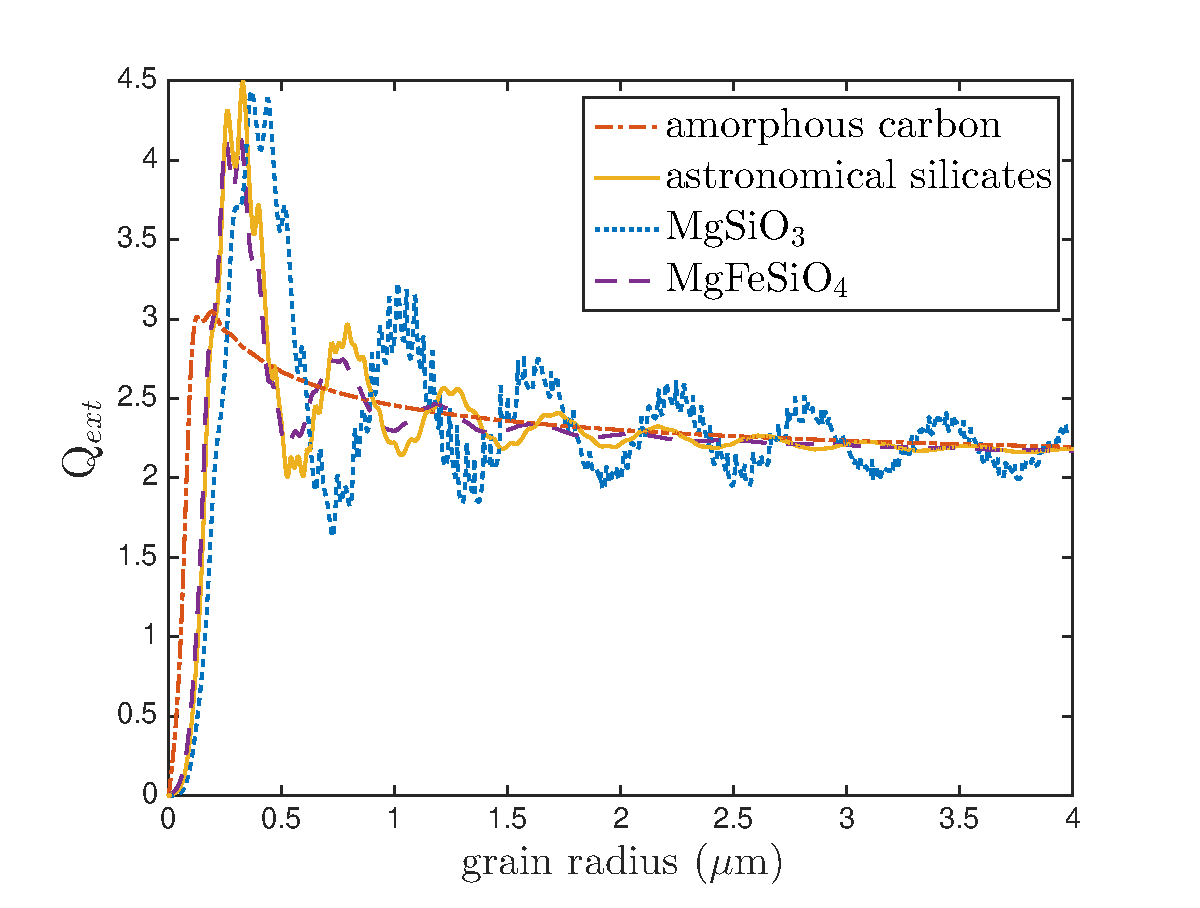
\includegraphics[trim =37 10 45 15,clip=true,scale=0.75]{chapters/chapter4/images/Qext_grainsize_upto4}
\end{subfigure}\\[1ex]
\begin{subfigure}{\textwidth}
\centering
\includegraphics[trim =35 10 45 15,clip=true,scale=0.75]{chapters/chapter4/images/Qext_grainsize_upto4_log}
\end{subfigure}
\caption{Variation of extinction efficiency ($Q_{ext}$) with grain size for amorphous carbon and silicates using Mie theory at $\lambda = 658 \mu $m. Optical constants are from \citet{Zubko1996} and \citet{Draine1984}. A linear scale is presented on the top and a log scale on the bottom.}
\label{Qext_grain}
\end{figure}

\begin{figure}
\begin{subfigure}{1\textwidth}
\centering
\includegraphics[trim =37 10 45 15,clip=true,scale=0.75]{chapters/chapter4/images/albedo_grainsize_upto4}
\end{subfigure}\\[1ex]
\begin{subfigure}{1\textwidth}
\centering
\includegraphics[trim =35 10 45 15,clip=true,scale=0.75]{chapters/chapter4/images/albedo_grainsize_upto4_log}
\end{subfigure}
\caption{Variation of albedo with grain size for amorphous carbon and silicates using Mie theory at $\lambda = 658 \mu $m. Optical constants are from \citet{Zubko1996} and \citet{Draine1984}. A linear scale is presented on the top and a log scale on the bottom.}
\label{albedo_grain}
\end{figure}

The dependence of the shape of the line profile in the optically thin dust case 
is described in Section \ref{analytics}.  However, the density profile 
also plays a significant role where there is even a small amount of 
absorption.  As previously discussed, at relatively small optical depths, 
a section of the flat-topped region is removed resulting in a peak at 
$-V_{min}$.  The shape of the profile in this region is significantly 
affected by the density profile.  Shallow density profiles (low $\beta$) produce a virtually 
linear variation in flux between $-V_{min}$ and $+V_{min}$.  For a fixed dust
optical depth, the steeper the distribution becomes, the more concave the 
profile becomes between $-V_{min}$ and $+V_{min}$, ultimately resulting in 
a clear shoulder to the profile at $+V_{min}$.  For extremely steep density
distributions this can result in a double peaked profile with 
trough to the red of $V=0$.  A illustration of the effects of variation of 
$\beta$ with $\tau$ on the profiles is shown in Figure \ref{bt}.

\subsection{Inferring properties of the dust from the models}

The presence of an extended red wing at large positive velocities in 
combination with increased extinction on the red side at smaller positive 
velocities can allow the values of $\tau$ and $\omega$ to be well 
constrained.  In this case it is possible to translate these values into a 
dust mass and average grain size respectively for a given species or combination of 
species using  optical properties and Mie theory (see Figures 
\ref{Qext_grain} and \ref{albedo_grain}).  In fact, it is the dust mass and average grain size 
that is varied within the code for a specified species or combination of 
species i.e. the dust optical depth and grain size are not varied directly.  It is therefore important to note that the use of different 
optical properties may substantially alter the inferred optical depths and 
albedos for a given species of specific grain size as has been noted 
previously (e.g. \citet{Owen2015}).



For amorphous carbon, the larger the grain size used the larger the albedo 
and the smaller the cross-section of absorption.  Larger masses of dust 
are therefore required to fit the same degree of absorption if a larger 
grain size is used.  This is in contrast to SED radiative transfer 
modelling where larger grain sizes generally result in less dust being 
required to fit the IR portion of the SED (W15).  These two techniques in 
tandem may therefore give excellent limits on grain sizes for different 
species or combinations thereof.

\begin{figure}
\begin{subfigure}{0.5\textwidth}
\includegraphics[trim =30 31 45 0,clip=true,scale=0.45]{chapters/chapter4/images/dustdep/a0_001_opt_thin_HaHbPad}
\end{subfigure}
\hspace{4mm}
\begin{subfigure}{0.5\textwidth}
\includegraphics[trim =59 31 45 0,clip=true,scale=0.45]{chapters/chapter4/images/dustdep/a0_001_opt_thick_HaHbPad}
\end{subfigure} \\[1ex]

\begin{subfigure}{0.5\textwidth}

\includegraphics[trim =30 31 45 0,clip=true,scale=0.45]{chapters/chapter4/images/dustdep/a0_1_opt_thin_HaHbPad}
\end{subfigure}
\hspace{4mm}
\begin{subfigure}{0.5\textwidth}
\includegraphics[trim =59 31 45 0,clip=true,scale=0.45]{chapters/chapter4/images/dustdep/a0_1_opt_thick_HaHbPad}
\end{subfigure} \\[1ex]

\begin{subfigure}{0.5\textwidth}
\includegraphics[trim =30 0 45 15,clip=true,scale=0.45]{chapters/chapter4/images/dustdep/a1_opt_thin_HaHbPad}
\end{subfigure}
\hspace{3mm}
\begin{subfigure}{0.5\textwidth}
\includegraphics[trim =51 0 45 15,clip=true,scale=0.45]{chapters/chapter4/images/dustdep/a1_opt_thick_HaHbPad}
\end{subfigure}
\caption{Model line profiles for H$\alpha$ (6563\AA\ in red), H$\beta$ (4861\AA\ in yellow) and Pa$\delta$ (10049\AA\ in blue) for optically thin and  optically thick cases on the left-hand side and right-hand side respectively.  All models adopted density profile $\rho(r) \propto r^{-4}$ (i.e. $\beta = 2$), velocity profiles $v(r) \propto r$ and radii ratio $R_{in}/R_{out}=0.2$.  The grain radii used were $a=0.001~\mu$m (top), $a=0.1~\mu$m (middle) and $a=1.0~\mu$m (bottom). All the above models used amorphous carbon.}
\label{wav_dep}
\end{figure}

\begin{figure}
\begin{subfigure}{\textwidth}
\centering
\includegraphics[trim =30 30 45 25,clip=true,scale=0.55]{chapters/chapter4/images/Qabs_a0_001}
\end{subfigure} \\[0.5ex]

\begin{subfigure}{\textwidth}
\centering

\includegraphics[trim =30 30 45 25,clip=true,scale=0.55]{chapters/chapter4/images/Qabs_a0_1} 
\end{subfigure} \\[0.5ex]

\begin{subfigure}{\textwidth}
\centering
\includegraphics[trim =30 10 45 25,clip=true,scale=0.55]{chapters/chapter4/images/Qabs_a1_0}
\end{subfigure}
\caption{The variation of amorphous carbon dust absorption efficiency with grain size. The grain radii plotted are $a=0.001~\mu$m (top), $a=0.1~\mu$m (middle) and $a=1.0~\mu$m (bottom).  The vertical lines mark the wavelengths of H$\alpha$ (6563\AA\ in red), H$\beta$ (4861\AA\ in yellow) and Pa$\delta$ (10049\AA\ in blue).}
\label{wav_dep2}
\end{figure}






\subsection{Observable signatures of dust in line profiles}
\label{asym}

The greater the dust optical depth, the more attenuation of the line 
is observed.  As expected, the red side of the profile suffers a greater 
degree of absorption than the blue side.  The resulting asymmetry is 
somewhat more complex than perhaps previously thought however.  Dust has 
repeatedly been cited as the agent responsible for the apparent 
blue-shifting of line profiles in supernovae in the manner of the profiles 
presented in Figure \ref{fig:Lucy}.  That is, relatively high optical 
depths result in an overall shift of the entire profile towards the blue.

In practice a relatively large optical depth ($\tau \approx 2$) is 
required to actively shift the peak of the profile bluewards of its natural 
$V_{min}$ value corresponding to the velocity at the inner radius of the shell.  In most cases it seems more likely that the dust
may not be optically thick and the blue-shifting of the peak of the profile is 
likely a result of attenuation in the flat-topped section (close to 
$R_{in}$).  The peak would therefore tend to be located at $-V_{min}$.

Since dust absorption is wavelength dependent for $2\pi a < \lambda$, one might expect the 
position of the peak flux to be dependent on the wavelength of the line being 
considered.  The relationship between the locations of the peaks 
of profiles and their wavelength has been discussed by several authors in 
relation to dust formation \citep{Smith2012, Fransson2013, Gall2014}.  Whilst this may occur in cases of high dust 
optical depth, this is not necessarily likely to be seen in the ejecta of 
most supernovae.  The wavelength-dependence of dust absorption instead 
can result in differing degrees of extinction in the flat-topped region of 
each profile but still leave the peak at its blue-shifted position of 
$-V_{min}$.  Of course, the value of $V_{min}$ may be different for 
different species.  However, if this is the case then there would be no 
reason to expect a variation in the position of the peak of profiles to be 
correlated with the wavelength dependence of dust.  Rather one would 
expect it potentially to trace the location of different ions within the ejecta. 
However, for lines from the same ion, for example the Balmer and Paschen lines of HI,
I might expect to see peaks at the same position but differing degrees of absorption.
At high resolutions, it might be possible to detect differences in the shape of the line 
profiles, particularly between $-V_{min}$ and $+V_{min}$ where the steepness of the 
incline traces the degree of dust absorption.  This can be seen in Figure \ref{wav_dep} 
where I illustrate the effects of the wavelength dependence of dust absorption for 
three lines, H$\alpha$ (6563\AA), H$\beta$ (4861\AA) and Pa$\delta$ (10049\AA).  
All lines were modelled using three different grain sizes and in both optically thin and 
thick cases.  I also show the variation of the absorption cross-section with 
wavelength at three different grain sizes in Figure \ref{wav_dep2}.

The attenuation of the flat-topped region is  often such that it can 
be hard to discern a difference in slope between the attenuated 
section between $-V_{min}$ and $+V_{min}$ and the slope of the wing for 
$V>+V_{min}$, particularly in circumstances where data is of poor 
resolution or has a poor signal-to-noise ratio.  Even in the case of 
excellent data, it may be easy to overlook these particular features or to 
dismiss them as natural fluctuations in the geometry of the ejecta rather than 
that they may be a product of dust absorption effects.

The greater attenuation of radiation received from the receding portion of 
the ejecta results in an asymmetry of the line profile whereby the 
majority of the observed emission is located bluewards of the peak.  
However, the effects of repeated dust scattering events within the 
ejecta can serve to counter this asymmetry.  Even in the case of dust grains 
with a relatively low albedo, a surprisingly persistent wing on the red 
side of the profile is seen beyond the maximum theoretical velocity 
of the emitting region.  For higher albedos this can actively result in a 
shift in the overall asymmetry of the profile, with the majority of the 
emission being emitted redwards of the peak, though the peak itself 
remains blue-shifted.

This effect is obviously analogous to that of electron scattering which 
also produces a significant red wing in line profiles \citep{Hillier1991, 
Auer1972}. This is an important consideration in both modelling and 
analysis of spectral line profiles.  DAMOCLES has the capacity to include 
a basic electron scattering mechanism in order to assess the possibility 
that any observed red wing might be produced by electron scattering rather 
than dust scattering.  The red wing observed in line profiles is an 
excellent diagnostic for determining the overall dust albedo and it is 
therefore important to establish whether this feature is due to 
electron or dust scattering or a combination of the two.

The combination of relatively low optical depths, initially flat-topped 
profiles, greater attenuation on the blue side with increased flux on the 
red side due to scattering can result in a profile that ends up appearing 
almost symmetrical, particularly if 
contaminants, such as narrow lines or blending with other broad lines, are 
present or if the resolution of the data is low.  The potential for apparently 
symmetrical profiles that appear to have been uniformly blue-shifted 
should be noted (see Figures \ref{bt} and \ref{wt} for examples of this).



\subsection{The effect of a grain size distribution}
\label{gs_distn}
It is important to consider the potential effect on the dust mass of modelling a grain size distribution instead of a single grain size.  For a grain size distribution the overall extinction cross section, $C_{ext}$, at a given wavelength is calculated as

\begin{equation}
C_{ext}=\int^{a_{max}}_{a_{min}} Q_{ext}(a) n(a) \pi a^2 da 
\end{equation}

where $Q_{ext}(a)$ is the extinction efficiency for a grain size $a$ and $n(a)$ is the number of grains with size $a$. The overall extinction efficiency is then

\begin{equation} 
Q_{ext} = \frac{C_{ext}}{ \int^{a_{max}}_{a_{min}} n(a) \pi a^2 da} 
\end{equation}
 
The scattering cross-section $Q_{sca}$ is similarly calculated.  As a result of these calculations, there is rarely a single grain size that has the same albedo and extinction efficiency as a size distribution.  Modelling a size distribution instead of a single grain size may therefore alter the deduced dust mass.  Since models are only sensitive to the optical depth and the albedo, however, it is not possible to deduce the grain size range or distribution and only single grain sizes are investigated in the models that are presented in the following chapters.

Whilst this apparently limits the scope of these results, it is important to consider the extent to which considering grain size distributions would alter the derived dust masses.  By considering a number of grain size ranges and adopting a power law distribution with a variable exponent, I may gain some insight into the effects of adopting a distribution rather than a single size.  For the classical MRN power law ($n(a) \propto a^{-3.5}$) with a wide grain size range ($a_{min} = 0.001 \mu$m to $a_{max} = 4.0 \mu$m) the derived albedo of $\omega=0.001$ is much too small to reproduce the required wing seen at early epochs.  I investigate this issue by adjusting the exponent of a distribution for a number of grain size ranges until the overall albedo is the same as that seen for the best fitting single grain size.  I can then approximately calculate the required dust mass for a distribution of grain sizes from the properties of a single-size model by equating the optical depths.  The optical depth for a single grain size is proportional to 

\begin{equation}
\tau \propto Q_{ext}(a)  \sigma(a) n_d
\end{equation}

\noindent where $n_d$ is the number density of dust grains, $\sigma(a)$ is the cross-sectional area of a grain of radius $a$ and $Q_{ext}(a)$ is the extinction efficiency for a grain of radius $a$.  On average, this gives

\begin{equation}
\tau \propto \frac{Q_{ext}(a) M \pi a^2}{\frac{4}{3} \pi a^3 \rho V}
\end{equation}

\noindent for a total dust mass $M$, total volume of the ejecta $V$ and density of a dust grain $\rho$.

This simplifies to 

\begin{equation}
\tau \propto \frac{Q_{ext}(a) M}{\frac{4}{3} a \rho V}
\end{equation}

\begin{equation}
\label{distn_conv}
M_{d}= \frac{M_s Q_{ext,s}(a_s)}{a_s} \times \frac{\int^{a_{max}}_{a_{min}} n(a) a^3 da}{\int^{a_{max}}_{a_{min}} Q_{ext}(a) n(a) a^2 da}
\end{equation}

where the subscript $s$ represents the single grain size quantities and the subscript  $d$ represents quantities for the grain size distribution.  This is only calculable for a specific wavelength and is therefore only an approximate conversion when performed at the rest-frame wavelength of the line in question.  However, practically, the variation of extinction efficiency and albedo over the narrow wavelength ranges modelled within the code is not significant and so this method produces relatively accurate dust masses (as determined by running models with the new parameters).

\subsection{The effect of different species}

In the majority of the modelling that follows, a single species, amorphous carbon, is considered.   A single species is used since the parameters that affect the quantity of dust required in the model are the albedo and the optical depth.  There are therefore  likely many possible combinations of species that may result in a good fit to the data.  The choice of amorphous carbon is partly motivated by evidence that, for SN~1987A (which, as an incredibly well-observed and relatively typical core-collapse supernova, is an excellent test case) the fraction of silicates present in the dusty ejecta is limited to approximately 15\% (W15, \citet{Ercolano2007}).  It is also motivated by previously published SED models which generally employ amorphous carbon.  This is because SED models frequently require far larger masses of silicate dust than amorphous carbon dust in order to produce similar levels of infrared flux and therefore amorphous carbon models are likely to produce the more conservative dust mass estimates.  By modelling with amorphous carbon I may compare directly to these models where possible.

I consider the change in dust mass when a medium of 100\% silicates is used instead of amorphous carbon.  I use optical constants presented in \cite{Draine1984}.  In a similar manner to the approach detailed in Section \ref{gs_distn}, I may calculate the mass of silicates that is equivalent to a carbon mass for a single grain size.  I consider the albedo at the original grain size, calculate the equivalent grain size for silicates that results in the same albedo and then calculate the new dust mass by considering the change in the extinction efficiency as

\begin{equation}
M_{sil} = M_{amc} \Big( \frac{Q_{amc}}{Q_{sil}} \Big) \Big(\frac{a_{sil}}{a_{amc}}\Big) \Big(\frac{\rho_{sil}}{\rho_{amC}}\Big)
\end{equation}

Because of the nature of the variation of albedo with grain size for silicates (see Figure \ref{albedo_grain}), there is often more than one silicate grain size that will give rise to the same albedo.  I consider all the possibilities and the resulting mass conversion factors in Table \ref{tb_sil}.  In my best fitting models for days 714 and 806, using any fraction of silicates of either grain size would serve to increase the dust mass.  However, at later epochs, using some fraction of silicate dust would reduce the dust mass to potentially more than half of my estimated values. However, this is still within my predicted range and my minimum and maximum dust masses remain robust.

\begin{table}
	%\begin{minipage}{180mm}
	\caption{Equivalent dust masses for the day 714 clumped models using grain size distributions and 100\% amorphous carbon. $f$ is factor of increase from the dust mass for the single size model ($M=7 \times 10^{-5} M_{\odot}$ with $a=0.6 \mu$m) and $p$ is the exponent of the grain size distribution $n(a) \propto a^{-p}$.}
	\label{tb_sil}
	\begin{center}
  	\begin{tabular}{@{} cccccc @{}}
    	\hline
	\multicolumn{2}{c}{\textit{carbon}} && \multicolumn{2}{c}{\textit{silicates}} & \\
$a$ & $Q_{ext}$ & &$a$& $Q_{ext}$ & $f=M_{sil}/M_{amc}$ \\
\hline
0.6 & 2.60633 & &0.0583 & 0.0772 & 5.37 \\
0.6 & 2.60633 & &4 & 2.1828 & 13 \\
 \\
3.5 & 2.2129 & &0.0641 & 0.10182 & 0.65 \\
3.5 & 2.2129 & &1.02 & 2.149 & 0.49 \\
3.5 & 2.2129 & &1.376 & 2.3514 & 0.61 \\


    \hline
  \end{tabular}
  \end{center}
%\end{minipage}
\end{table}

\subsection{The velocity distribution}
\label{scn:vel_prof}









%\clearthesisemptydoublepage
\chapter{The Evolution of Dust Formation in SN~1987A}\label{chp:chp5}

%\begin{flushright}
%  {\em QUOTE GOES HERE }\\
%
%\ \

%\normalsize
%{AUTHOR}  
%\end{flushright}



On 23 February 1987, a star died in an explosion that would inform our understanding of core-collapse supernovae for decades to come.  SN~1987A is uniquely important to the study of supernovae.  At only 50 kpc away in the Large Magellanic Cloud (LMC) and as the brightest supernova to be observed since SN 1604 (Kepler), it has provided an unprecedented opportunity for studying every aspect of supernovae.  Since its discovery by Ian Shelton and Oscar Duhalde at Las Campanas, Chile \citep{Kunkel1987}, SN~1987A has been continuously observed across the entire wavelength range, providing astronomers with a wealth of data and discoveries.  

SN~1987A was the first supernova to be detected via the emission of neutrinos.  Hours before the visible light from SN~1987A reached Earth, 19 neutrinos were simultaneously detected in various locations across the globe confirming the core-collapse theory of supernovae \citep{Bionta1987,Hirata1987}.  However, the neutron star that is expected to have resulted from this collapse has yet to be detected.  Various theories exist for this non-detection such as the possibility that a black hole formed instead of a neutron star or that dust is obscuring our view \citep{Brown1992}.

\begin{figure}
\centering
\includegraphics[clip=true,scale=0.4,trim= 20 80 20 40]{chapters/chapter5/images/87A_image.jpg}
\caption{SN~1987A in the Large Magellanic Cloud.  The three-colour image is composed of several pictures of the region taken with the Wide Field and Planetary Cameras on the Hubble Space Telescope between September 1994 and July 1997.  Image courtesy of NASA, ESA, and The Hubble Heritage Team (STScI/AURA).}
\label{87A_img}
\end{figure}

The detection of neutrinos in combination with the presence of hydrogen lines in the early spectra resulted in the classification of SN~1987A as a Type II supernova.  However, SN~1987A was unusually dim at peak magnitude compared to other Type II SNe and brightened very quickly, its magnitude increasing by a factor of 100 in just three hours compared to a normal timeframe of several days.  SN~1987A exhibited a number of other somewhat unusual features. Broad lines detected in the very early spectra indicated expansion velocities of up to 30,000~km~s$^{-1}$, much faster than the typical 15,000~km~s$^{-1}$. The colour evolution of the object was also faster than  expected.  These atypical properties suggested that the progenitor star was more compact than the red supergiants that are believed to normally give rise to Type II SNe.  In fact, four days after the initial detection of SN~1987A, the progenitor star was identified as having been the blue supergiant Sanduleak -69$^{\circ}$ 202  confirming this theory \citep{Sonneborn1987}.  These distinctive features, in combination with a plateauing light curve, led to the final classification of SN~1987A as a peculiar Type II-P supernova. 

\begin{figure}
\centering
\includegraphics[clip=true,scale=0.4,trim= 0 0 0 0]{chapters/chapter5/images/HST_ring.png}
\caption{Evolution of the ring collision from 1994 to 2014 from a combination of HST B- and R- band images.  The brightness of the ring has been reduced by a factor of 20 by applying a mask to the images making it possible to see the morphology of the ring at the same time as the faint ejecta.  The image is taken from \citep{Fransson2015}.}
\label{HST_ring}
\end{figure}

After the initial flash of ionising radiation in the first few hours \citep{Ensman1992}, the expanding debris of SN~1987A cooled rapidly, dropping from 14,000 K to 6,000 K between the first and tenth days after outburst \citep{Kirshner1987} before eventually stabilising at around 5,500 K.  By just four months after outburst, the debris were transparent in the optical and IR \citep{McCray1993}.  The ejecta spectrum was dominated by emission lines, often exhibiting P-Cygni profiles, arising from a blackbody-like continuum.  Numerous hydrogen, calcium and sodium lines could be seen in the optical as well as a rich spectrum of IR emission lines  from other heavy elements.  

The forward shock continued to propagate through the ejecta and by the mid 1990s reached the innermost of the beautiful and complex system of rings that are observed around SN~1987A (see Figures \ref{87A_img} and \ref{HST_ring}).  The rings were most likely caused by an ejection of mass following a binary merger some 20,000 years before SN~1987A exploded \citep{Morris2005,Fitzpatrick2013}.  This merger also likely explains the surprising blue colour of the progenitor star.  A series of images of the equatorial ring (ER) taken using the Hubble Space Telescope (HST)  clearly show the appearance of ``hot spots" as the dense material is shock-ionised on impact with the forward shock (see Figure \ref{HST_ring}).  The interaction of the forward shock with the ER has precipitated a strong reverse shock that is now travelling back through the ejected material \citep{Fransson2013}.  The illumination of the outer parts of the ejecta by the reverse shock is visible in spectra taken at later epochs as faster regions became more dominant in line profiles making them appear broader.  It has been suggested that this point in SN~1987A's evolution marks its transition to a remnant \citep{McCray2003}.

The ionisation and heating of the ejecta of the supernova is caused by gamma rays that result from the decay of $^{56}$Co, $^{57}$Co and $^{44}$Ti (with half lives of 77.3 days, 272 days and 59 years respectively \citep{Manuel2002}).  The gamma rays Compton scatter off electrons that are often bound causing the production of fast, primary photoelectrons. These primary electrons go on to impact atoms causing further ionisations and excitations. A population of secondary electrons is thus produced.  Recombinations and de-excitations result in the emission of monochromatic photons.  These emission lines are then broadened thermally and via the large bulk velocity of the emitting medium.  I present models of these optical and IR emission line profiles from SN~1987A throughout this chapter.  The ionisation state of the ejecta of SN~1987A is thought to reach a period of stability known as the ``freeze-out" when a balance is reached between the recombination and ionisation rates \citep{Danziger1991,Kozma1998a,Fransson2013}.  This is discussed in further detail later in this chapter as it has relevance to the evolution of the shapes of the line profiles.

A full review of SN~1987A in all its glory would likely extend to many dozen of pages and so in the following paragraphs I will focus only on those facets of the history of SN~1987A that relate to the formation of dust in its ejecta.  For extensive reviews covering the progenitor, the explosion mechanism, the dynamics and geometry, the light curves and spectral evolution, the thermodynamics, the chemistry and the circumstellar ring system I refer the reader to the reviews by \citet{Arnett1989}, \citet{McCray1993} and \citet{McCray2003}.  A comprehensive review of SN~1987A by Richard McCray encompassing its later evolution is due to be published next year \citep{McCray2016}.


\begin{figure}
\centering
\includegraphics[clip=true,scale=0.35,trim= 0 0 0 0]{chapters/chapter5/images/Herschel_img.png}
\caption{\textit{Herschel} images of SN~1987A.  Image taken from \citet{Matsuura2011}.}
\label{Herschel_img}
\end{figure}

\section{10,000 Days of Dust}
SN~1987A is the first and only supernova to have had the formation of dust in its ejecta traced via all three observable signatures described in Section \ref{three_sigs} \citep{Bouchet2014}.  Before dust was observed, its formation in the ejecta of SN 1987A was predicted.  \citet{Gehrz1987} recognised that conditions in the cooling ejecta would eventually reach temperatures and densities appropriate for dust formation to occur.  They predicted that the onset of dust formation would occur at around days 240-300.  This idea was expanded upon by \citet{Dwek1988} who estimated that dust would begin to form slightly later at around day 400 and might even cause an optical black-out of the supernova.

\begin{figure}
\centering
\includegraphics[clip=true,scale=0.31,trim= 0 0 0 0]{chapters/chapter5/images/ALMA_imgs.png}
\caption{ALMA, ATCA, HST and Chandra images of SN~1987A showing the location of the dust in the inner ejecta at 450~$\mu$m.  The image is taken from \citep{Indebetouw2014}.  Inset HST image courtesy of R. Kirshner and the SAINTS collaboration (also see \citet{Larsson2013}) and the inset Chandra X-ray image is from \citet{Helder2013}.}
\label{ALMA}
\end{figure}

The first indications of dust in the ejecta of SN~1987A appeared at around day 350 with the emergence of continuum radiation in the IR longward of 5~$\mu$m \citep{Meikle1993}.  This had become prominent by day 550 \citep{Roche1993,Wooden1993}.  It was suggested by some that this excess IR emission was the result of  a light echo reflecting off the circumstellar material \citep{Roche1989}.  However, at around day 530, the optical luminosity suddenly started dropping more rapidly than it had done previously.  The IR luminosity started to increase,  compensating for the drop in the optical and ensuring that the bolometric light curve continued to follow the same trajectory \citep{Suntzeff1991,Whitelock1991}.  At the same time it was observed that the peaks of several emission lines in the optical and IR had become shifted towards the blue indicating that the dust was indeed within the supernova envelope itself \citep{Lucy1989,Danziger1991a,Danziger1991,Meikle1991,Meikle1993,Suntzeff1991,Hanuschik1993}.  It was Leon Lucy and collaborators who first suggested that the presence of blue-shifted line profiles may indicate dust formation in the ejecta of supernovae and they even went as far as producing some models to illustrate the effects.  They used this method  to estimate for the first time the dust mass in the ejecta of SN~1987A ($10^{-6}M_{\odot} - 10^{-4}M_{\odot}$,  \citealt{Lucy1989,Lucy1991}).  Around this time, \citet{Wooden1993} also placed a lower limit of $\sim10^{-4}$~M$_{\odot}$ on the  dust mass in SN~1987A based on SED-fitting.

After this intensive monitoring of SN~1987A in the MIR, there was something of a gap in observations.  By the mid 1990s SN~1987A had faded and could no longer be detected in the mid-IR with current instruments.  It was not until 2004 that new instruments at the Gemini South telescope and at the Very Large Telescope allowed for the resumption of observations of SN~1987A at these wavelengths.  The first resolved detection of the central ejecta was reported by \citet{Bouchet2004} who observed the object at 10~$\mu$m and  $20$~$\mu$m. They estimated a  mass  of $10^{-4}M_{\odot}-2 \times 10^{-3}M_{\odot}$ for the dust in the ejecta, with an estimated temperature of $90K<T<100K$.  They concluded that CCSNe could potentially be a significant source of dust in the Universe but could not solely account for the masses seen at high redshifts (see Chapter \ref{chp:chp1}).  Subsequent observations continued to detect this faint mid-IR emission right up to the present day \citep{Dwek2010,Bouchet2014} whilst radiative transfer models of the SEDs continued to find dust masses of the order of $10^{-4}-10^{-3}M_{\odot}$ during the first 1000 days \citep{Ercolano2007}.

For many years it was assumed that only a small mass of dust, possibly as much as a few $\times 10^{-3}M_{\odot}$, had formed in the ejecta of SN~1987A within the first 1000 days.  It was not until the first \textit{Herschel} observations of SN~1987A that the picture suddenly changed.  SN~1987A had not been chosen as a target for the \textit{Herschel} mission as it was believed that it would not be detectable at far-IR and sub-mm wavelengths.  However, in 2010, whilst \textit{Herschel} was performing a survey of the LMC as a part of the HERITAGE survey \citep{Meixner2013}, an unexpectedly strong signal was detected in the same region as SN~1987A.  In 2011, \citet{Matsuura2011} published the first detections of the SN~1987A system at long wavelengths (100, 160, 250 and 350~$\mu$m presented in Figure \ref{Herschel_img}).  These observations revealed the presence of a massive reservoir (0.4 - 0.7 $M_{\odot}$) of cold dust ($17K<T<23K$) that they argued was located in the ejecta.  \textit{Herschel} did not have the angular resolution to determine the location of the emitting dust and as a result there was much contention over this assertion with many claiming that the detection was of pre-existing dust located in the circumstellar material \citep{Bouchet2014}.  However, follow-up observations of SN~1987A with the Atacama Large Millimetre Array (ALMA) published by \citet{Indebetouw2014} resolved the SN-ring system and revealed the location of the dust to be entirely within the ejecta (see Figure \ref{ALMA}).  Further pointed\textit{Herschel} observations corroborated the large estimated dust masses \citep{Matsuura2015}.  These dust mass estimates were all based on fitting dust spectral energy distributions (SEDs) that peaked at far-IR wavelengths.

The majority of the dust in the ejecta of SN~1987A is located centrally and as such has not yet encountered the reverse shock that is propagating back towards it.  Whilst it is now clear that very large masses of dust have indeed formed in the ejecta of SN~1987A, it remains unclear whether the dust will survive the passage of the reverse shock.  The composition of the dust and the size of the grains are crucial to understanding how much of the dust that has formed will actually be deposited into the ISM in the future.  Further observations and analyses of the dust mass present in the ejecta are  crucial to understanding how much dust is actually contributed to the ISM from CCSNe.




The {\em Herschel} mission ended in 2013 and there is now likely to be a long wait for far-IR facilities with comparable or better sensitivities than {\em Herschel} to become available.  The method of SED fitting is therefore unhelpful until other telescopes come into operation.  This provides a strong incentive to make use of alternative methods to estimate the dust masses that form in supernova ejecta.  Following the work of \citet{Lucy1989}, no further analysis of the shapes of the line profiles in SN~1987A has been performed.  With such a large database of spectral observations available, SN~1987A provides the perfect opportunity to assess the evolution of the formation of dust in the ejecta of CCSNe.  

\begin{figure}
\centering
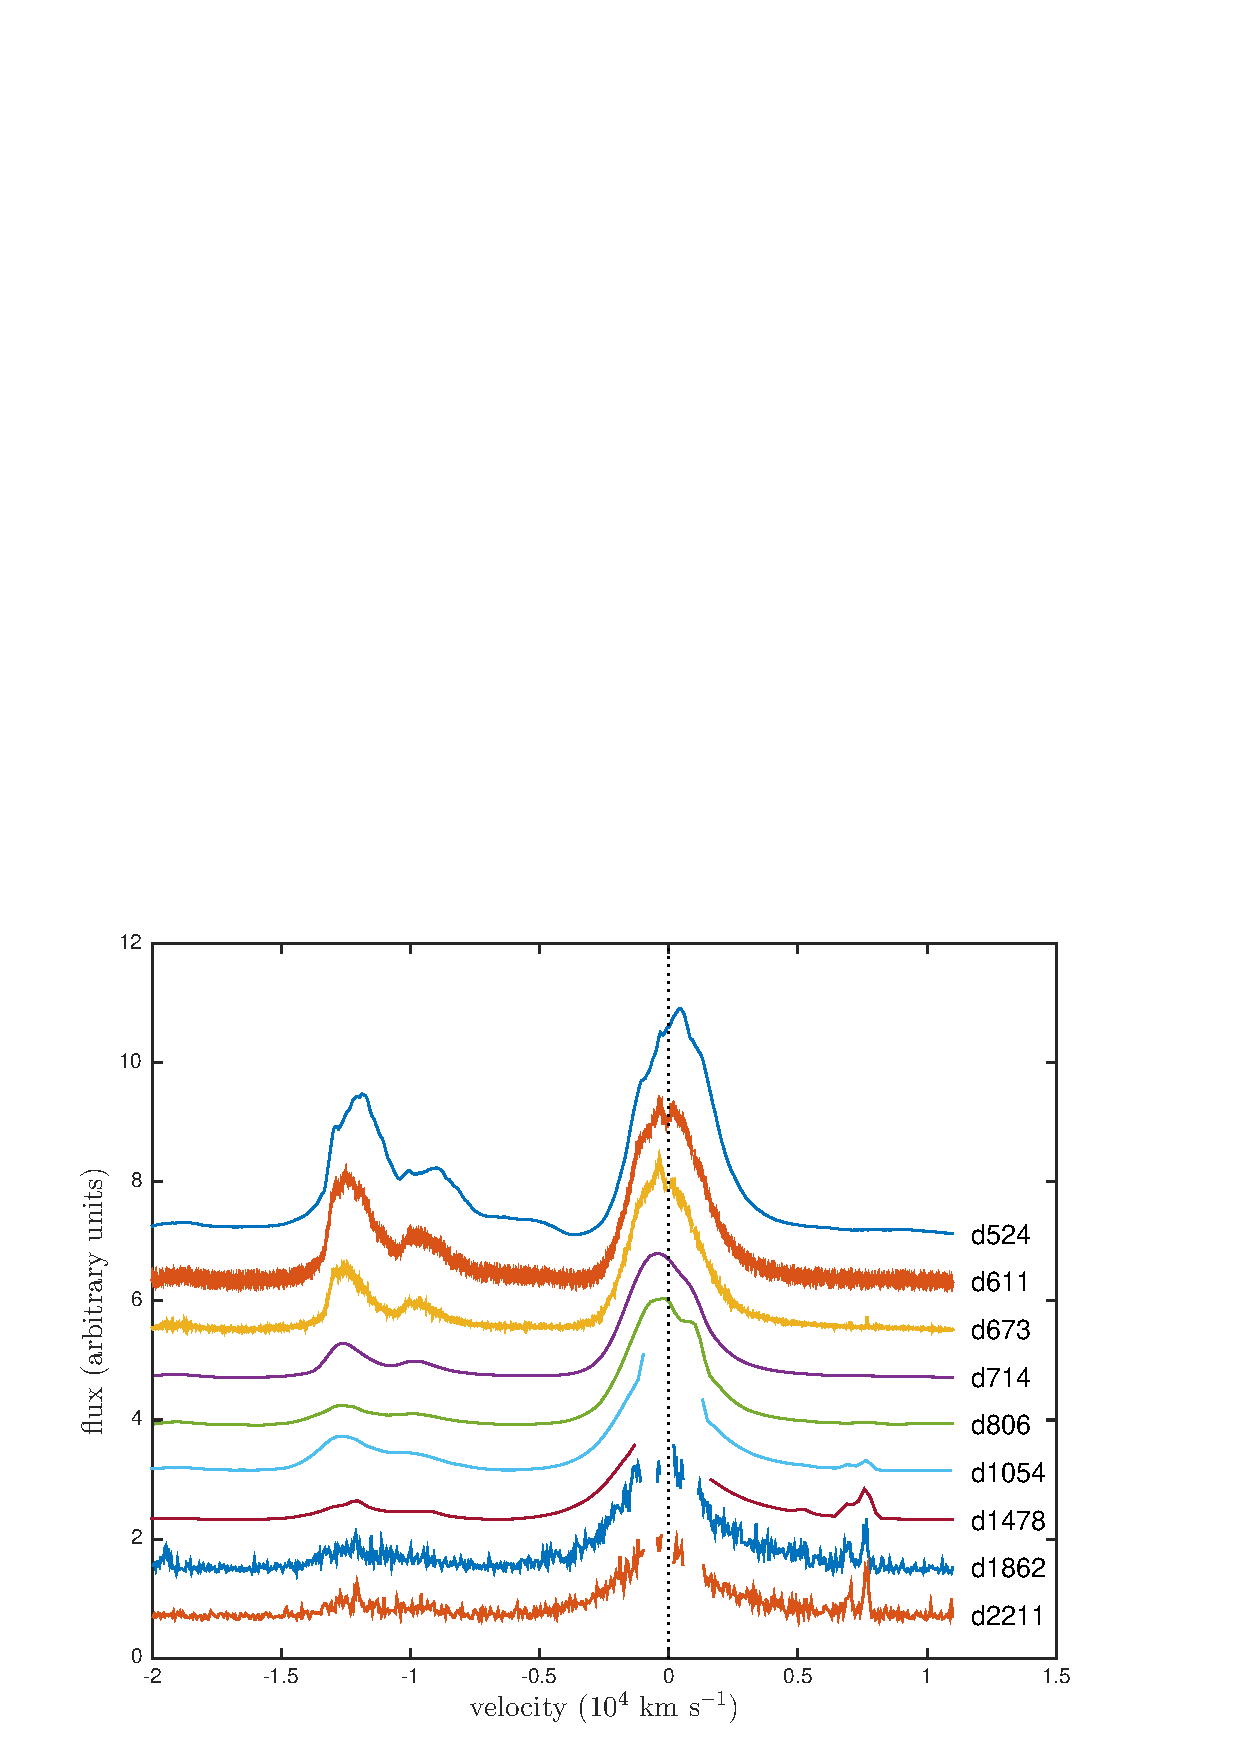
\includegraphics[trim =39 10 45 15,clip=true,scale=0.7]{chapters/chapter5/images/Ha_evol_early_1col2.pdf}
\caption{Archival data showing the evolution of the H$\alpha$ and
[O~{\sc i}] line profiles from SN~1987A at the earlier of the epochs considered. The 
spectral gaps at the last two epochs correspond to where narrow line 
emission from the equatorial ring has been removed. The spectra have been
continuum-subtracted and offsets have been applied for display purposes.}
\label{Ha_evol_early}
%\end{center}
\end{figure}

In this chapter, I present a number of models of line profiles of SN~1987A. I have collated optical spectra from the archives of four different telescopes in order to study the effects of dust formation on 
the H$\alpha$ line and on the [O~{\sc i}]$\lambda\lambda$6300,6363~\AA\ doublet.  
I have modelled epochs spanning a range of approximately 8 years, from the first 
indications of blue-shifting in the H$\alpha$ line between days 600-700, using 
both smooth and clumped geometries.  I compare my derived dust masses to 
those obtained by (\citealt{Wesson2015}, hereafter W15) and (\citealt{Dwek2015}, hereafter DA15) and consider the implied dust formation rate. 

In Section \ref{spectra}, I detail the observed spectra that I used for 
my modelling and I present my modelling of the 
H$\alpha$ and [O~{\sc i}]$\lambda\lambda$6300,6363~\AA\ lines in 
Section \ref{results}.  Finally, I discuss my findings in Section 
\ref{discuss}.
    


\begin{figure}
\centering
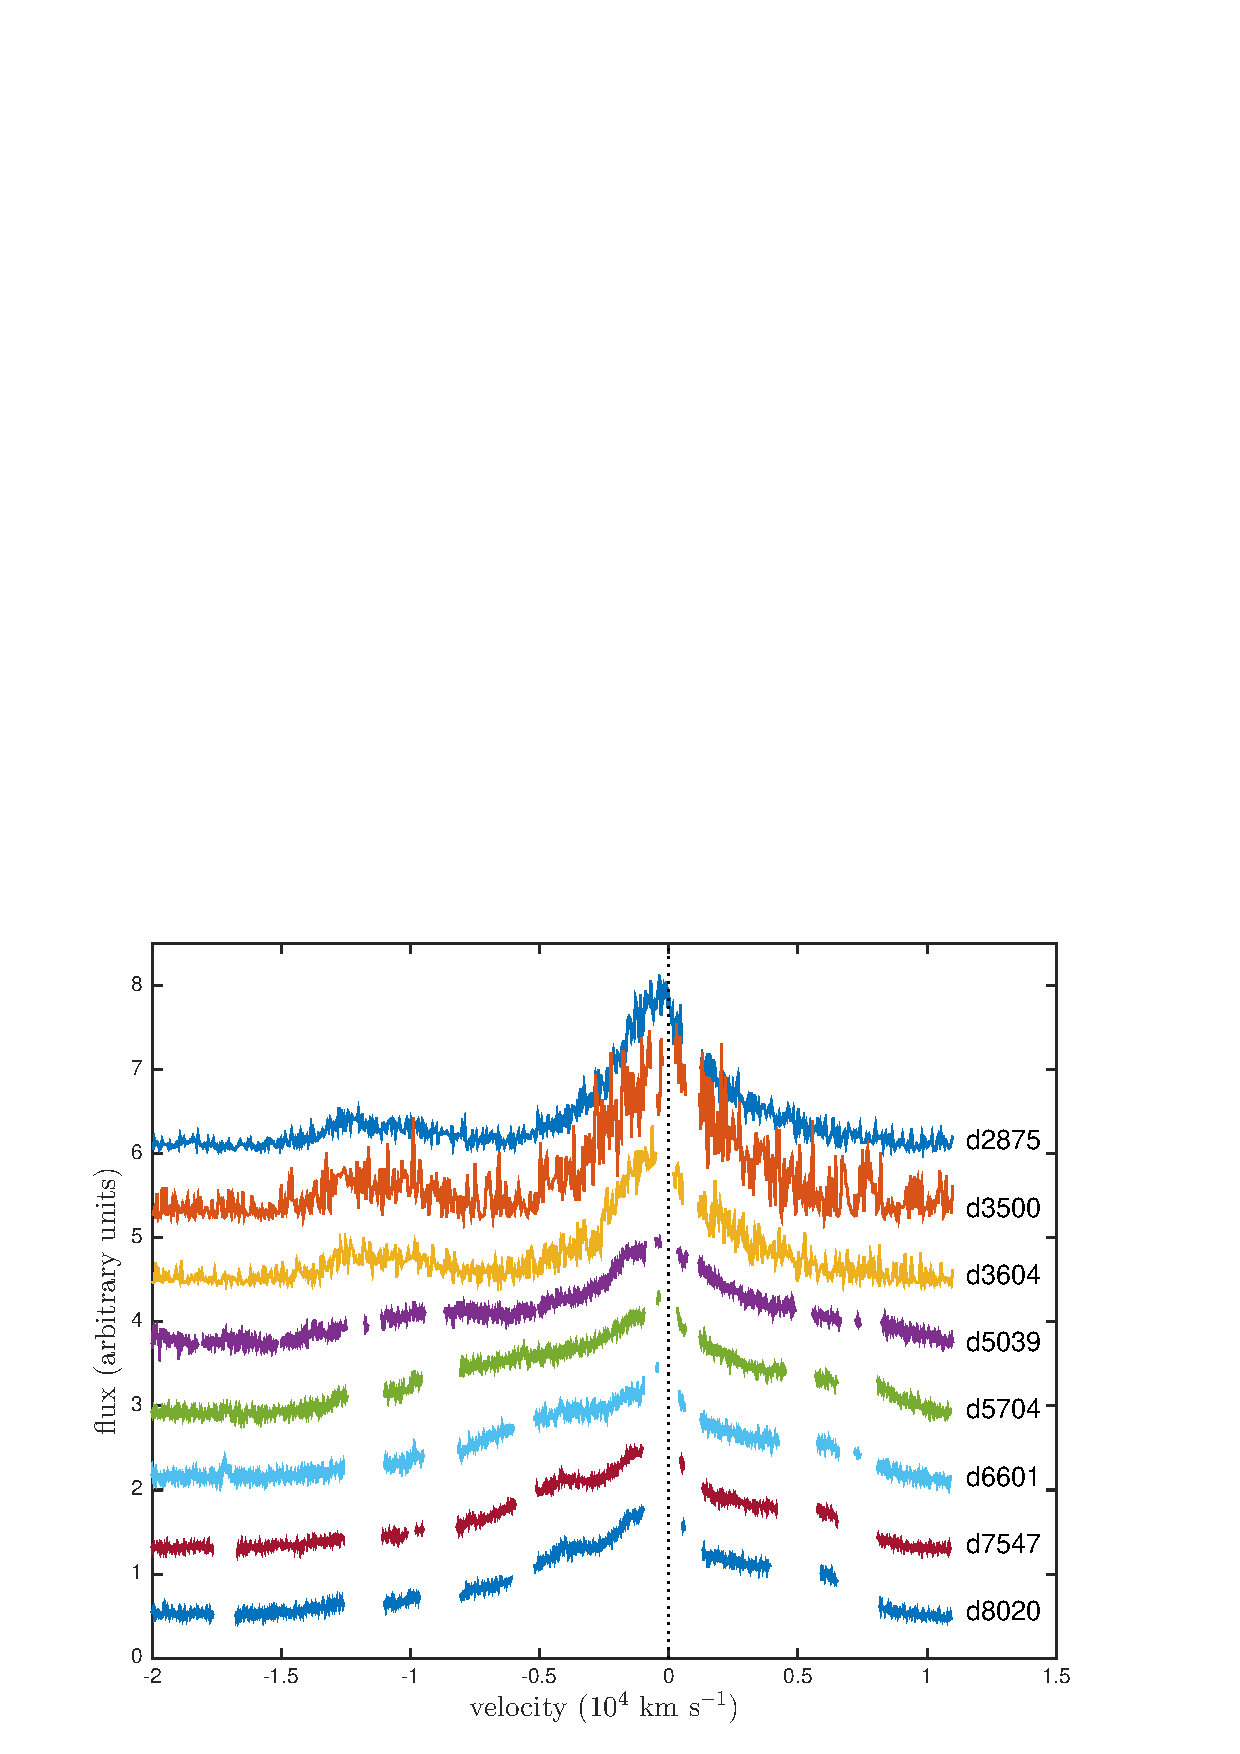
\includegraphics[trim =45 10 45 15,clip=true,scale=0.7]{chapters/chapter5/images/Ha_evol_late_1col.pdf}
\caption{Archival data showing the evolution of the H$\alpha$
line profile from SN~1987A at the later epochs. The spectral gaps 
correspond to where narrow line emission from the ER has been 
removed. The spectra have been continuum-subtracted and offsets applied 
for display purposes.}
\label{Ha_evol_late}
%\end{center}
\end{figure}
%FIGURE


\afterpage{
\begin{landscape}
\setlength{\tabcolsep}{7pt}
\begin{table}
%	\begin{minipage}{180mm}
	\centering
	\caption{Details of the archival data for SN~1987A.}
	\label{tb:data}
  	\begin{tabular}{@{} ccccccccl @{}}
    	\hline
	Date & Age & Telescope  & Inst & $\lambda_{min}$ & $\lambda_{max}$ & Res. & Res. & Reference \\
	& (days) & & &(\AA) & (\AA)& (\AA) & Power\\
	\hline
31 Jul 1988 & 524 & AAT & FORS & 5500 & 10190 & 20 & & \citet{Spyromilio1991} \\
26 Oct 1988 & 611 & AAT & UCLES & 6011 & 7336 &  & 30000 & \citet{Hanuschik1993, Spyromilio1993}\\
27 Dec 1988 & 673 & AAT & UCLES & 5702 & 10190 &  & 30000 & \citet{Hanuschik1993, Spyromilio1993}\\
06 Feb 1989 & 714 & CTIO-1.5m & Cass. & 6420 & 10380 & 16 & & \citet{Phillips1990}\\
09 May 1989 & 806 & CTIO-1.5m & Cass. & 6430 & 10330 & 16 & & \citet{Phillips1990}\\
12 Jan 1990 & 1054 & CTIO-4m & RC & 3565 & 10000 & 11 & & \cite{Suntzeff1991} \\
12 Mar 1991 & 1478 & CTIO-4m & RC & 3245 & 9175 & 11 & & \\
30 Mar 1992 & 1862 & HST & STIS & 4569 & 6818 & 4.4 &  & \citet{Wang1996}\\
14 Mar 1993 & 2211 & HST & STIS & 4569 & 6818 & 4.4 &  & \citet{Wang1996}\\
07 Jan 1995 & 2875 & HST & STIS & 4569 & 6818 & 4.4 &  & \citet{Chugai1997}\\
23 Sep 1996 & 3500 & HST & STIS & 4569 & 6818 & 4.4 &  \\ 
05 Jan 1997 & 3604 & HST & STIS & 4569 & 6818 & 4.4 &  \\
10 Dec 2000 & 5039 & VLT & UVES & 4760 & 6840 &  & 50000 & \citet{Groeningsson2006, Groeningsson2007}\\
06 Oct 2002 & 5704 & VLT & UVES & 4760 & 6840 &  & 50000 & \citet{Groeningsson2006, Groeningsson2007, Groningsson2008}\\
21 Mar 2005 & 6601 & VLT & UVES & 4760 & 6840 &  & 50000 &\citet{Groeningsson2006, Groeningsson2007}\\
23 Oct 2007 & 7547 & VLT & UVES & 4760 & 6840 &  & 50000 & \citet{Groeningsson2007}\\
07 Feb 2009 & 8020 & VLT & UVES & 4800 & 6800 &  & 50000 & \citet{Tziamtzis2010}\\
    \hline
  \end{tabular}
%\end{minipage}
\end{table}
\end{landscape}
}
\setlength{\tabcolsep}{12pt}


\section{Spectral Observations of SN~1987A}
\label{spectra}
%This is just the archival spectra section of the paper

%%%%%%%%%%%%%%%%%%%%   SPECTRA   %%%%%%%%%%%%%%%%%%%%%%%%%%%

SN~1987A has been the most intensively observed supernova in history, with 
an abundance of both spectral and photometric data available to model.  From 
the archives of a number of different telescopes I have collated optical 
spectra acquired over a wide range of epochs.  At the earlier epochs I 
use spectra obtained by the Anglo-Australian Telescope (AAT) and the Cerro 
Tololo Inter-American Observatory (CTIO) and at later epochs I 
use spectra from the archives of the Hubble Space Telescope (HST) and the Very 
Large Telescope (VLT).  An explosion date of 23 February 1987 is adopted 
throughout and epochs are measured relative to this date.  Full details of 
all observations may be found in Table \ref{tb:data}. The spectral 
resolutions of the grating spectrograph observations are listed in 
column~7, while column~8 lists the spectral resolving powers of the 
echelle spectrograph observations.


Wavelength ranges encompassing the H$\alpha$ line and [O~{\sc 
i}]~$\lambda$6300,6363~\AA\ doublet were selected in order to trace their 
evolution from day 524, near the time of the first indications of dust 
formation \citep{Wooden1993}, to day 8020, near the current era. Optical 
spectroscopy obtained at the AAT using the Faint Object Red Spectrograph 
(FORS) during the first two years after outburst was kindly supplied by Dr 
Raylee Stathakis \citep{Spyromilio1991, Hanuschik1993, Spyromilio1993} and 
optical spectra from the CTIO were donated by Dr Mark Phillips 
\citep{Suntzeff1991}.

The evolution of the H$\alpha$ and [O~{\sc i}] line profiles is presented 
in Figures \ref{Ha_evol_early} and \ref{Ha_evol_late}.  At later epochs, 
the broad H$\alpha$ profile emitted by the ejecta becomes contaminated by 
narrow line emission from the ER.  These lines have been 
removed for the purposes of modelling the broad line. A continuum fit has 
been subtracted from each spectrum and a velocity correction has been 
applied for a recession velocity of 287 km~s$^{-1}$ 
\citep{Groningsson2008}.




\subsection{Contamination of the H$\alpha$ Profiles}

The H$\alpha$ profile at day 714 exhibits a very slight inflection visible 
at $V \approx +900$ km~s$^{-1}$.  By day 806, this slight inflection has 
developed into a noticeable shoulder in the line profile of H$\alpha$ (see 
Figure \ref{Ha}).




Although these features are similar in nature to features produced by dust 
absorption in the flat-topped region (as discussed in Section \ref{beta}), 
I conclude that this shoulder is an early appearance of the unresolved 
[N~{\sc ii}] $\lambda$6583~\AA\ line from the ER \citep{Kozma1998b}.  Unresolved nebular [N~{\sc ii}] lines at $\lambda=$ 6583~\AA\ and 
$\lambda=$ 6548~\AA\ either side of the H$\alpha$ rest frame velocity at 
6563~\AA\ are certainly seen by day 1054 
%(see Figure \ref{d1054}) 
and have to be removed in order to consider the evolution of the broad 
H$\alpha$ profile (see Figure \ref{Ha_evol_early}). I do not remove this 
potential contaminant at earlier epochs but try to fit the broad line 
profiles around it.

 

\begin{figure}
\centering
\includegraphics[clip=true,scale=0.6,trim= 0 0 0 0]{chapters/chapter5/images/d1054Ha}
\caption{The low resolution H$\alpha$ line profile from SN~1987A observed at the CTIO on day 1054.  The unresolved narrow nebular [N~{\sc ii}] lines at $\lambda=$ 6583~\AA\ and $\lambda=$ 6548~\AA\ and the narrow nebular H$\alpha$ line at $\lambda=$6563~\AA\  can be clearly seen.}
\label{d1054_Ha}
\end{figure}
 
By day 1054, all three of the narrow nebular lines (H$\alpha$ and N[{\sc ii}]) are strong.  They 
remain unresolved in the low spectral resolution CTIO data at days 1054 
and 1478 and therefore contaminate the entire central region of the 
H$\alpha$ line profile (see Figure \ref{d1054_Ha}).  Their presence renders two CTIO H$\alpha$ 
profiles from days 1054 and 1478 unusable for modelling purposes.  The HST 
and VLT H$\alpha$ profiles at later epochs ($\ge$ 1862 days) have a higher 
spectral resolution and it was therefore easier to remove the narrower 
[N~{\sc ii}] and H$\alpha$ lines from the broad H$\alpha$ profiles (for 
example Figures \ref{Ha_evol_early} and \ref{Ha_evol_late}). Although this 
does remove a potentially informative section of the profile ($+500$ 
km~s$^{-1}<v<+1500$ km~s$^{-1}$), I achieve good fits to the overall line 
profiles at these epochs.

\begin{table}
\centering
\caption{H$\alpha$ full-width half-maxima (FWHM) and the half-width zero 
intensities (HWZI) in km s$^{-1}$ determined by the zero intensity velocity on the 
blue side of the line.  The tabulated line widths have been corrected for the relevant instrumental resolution.}
\begin{tabular}{c cc}
day & FWHM (km s$^{-1}$) & HWZI (km s$^{-1}$) \\
\hline
524 & 3200 & 3600 \\
611 & 2700 & 3400 \\
673 & 1600 & 3700 \\
714 & 3100 & 4500 \\
806 & 3200 & 5500 \\
1054 & 2100 & 5600 \\
1478 & 1400 & 6600 \\
1862 & 1600 & 6800 \\
2211 & 1400 & 6700 \\
2875 & 2700 & 6700 \\
3500 & 3500 & 7000 \\
3604 & 2100 & 7000

\end{tabular}

\label{FWHM}
\end{table}%

\subsection{The Evolution of the Maximum and Minimum Velocities}

For a freely expanding medium, the velocity of any fractional radial 
element should not change with time.  The maximum velocity of any 
line-emitting region is therefore expected to be constant.  However, at 
the epochs I consider here, it appears that the maximum velocities of the 
H$\alpha$ line, as determined by the velocity at zero intensity on the 
blue side, generally increase over time (see Table \ref{FWHM}).  I 
attribute this to the start of the freeze-out phase in the outer regions 
of the ejecta, while the hydrogen neutral fraction is still increasing in 
the denser inner regions \citep{Danziger1991,Fransson1993}.

The onset of a fixed ionisation structure in the ejecta causes the rate of 
H$\alpha$ flux decline to slow.  Since the outer, faster moving regions 
reach this state at earlier times than the inner, slower moving regions, 
the relative flux contribution of the outer regions is increased.  At 
early epochs ($t<900$ days) the flux contribution from hydrogen in the 
core dominates the overall H$\alpha$ flux, whereas at later epochs ($t > 
900$ days) the flux from the envelope dominates \citep{Fransson1993, 
Kozma1998a}.  This shift likely explains apparent broadening of the line 
with the higher velocity material becoming increasingly noticeable in the 
line profiles.  This may also explain the increase in half-width zero intensity (HWZI) velocities at 
these epochs with the relative flux from the very densest regions dropping 
more rapidly relative to the outer line-emitting region. The full-width 
half maximum (FWHM) remains relatively steady (see Table 
\ref{FWHM}). However, the FWHM values presented in Table \ref{FWHM} were difficult 
to determine accurately since the peak of the broad line profile is 
contaminated by narrow line emission from the ER.

%%%%%%%%%%%%%%%%%%%%   SPECTRA   %%%%%%%%%%%%%%%%%%%%%%%%%%%

\section{Modelling SN~1987A}
\label{results}





I have modelled the H$\alpha$ line of SN~1987A at days 714, 806, 1862, 
2211, 2875, 3500 and 3604, and the [O~{\sc i}]$\lambda\lambda$6300,6363~\AA\ 
doublet at days 714, 806, 1054 and 1478.  After day 3604 the H$\alpha$ 
profile begins to become dominated by emission from the reverse shock and 
the structure of the emitting region may no longer be approximated by a 
single shell model as I do here \citep{Fransson2013}.  The [O~{\sc 
i}]~$\lambda$6300,6363~\AA\ doublet becomes too weak to model after day 
1478 (see Figure \ref{Ha_evol_early}).  I continue to adopt a velocity 
profile $V(r) = \frac{V_{max}}{R_{max}}r$ and treat the variable 
parameters listed at the start of Section \ref{param_sens_analysis}.  Whilst the albedo and 
optical depth are not varied directly, they are altered by adjusting the 
dust mass, $M_{dust}$, and the grain radius, $a$, which together determine 
the albedo and optical depth via Mie theory and the optical properties of 
the dust.

\setlength{\tabcolsep}{10pt}
\begin{table}
\caption{Observed luminosities of the H$\alpha$ line and estimated 
electron scattering optical depths from $R_{in}$ to $R_{out}$ for the 
radii detailed in Tables \ref{smooth1} and \ref{clumped1} based on an 
assumed gas temperature of 10,000~K.}
\centering
\begin{tabular}{@{}cccccc@{}}
\hline
& \multicolumn{2}{c}{H$\alpha$} &  \multicolumn{2}{c}{[O~{\sc i}]}  \\
day &  $L_{obs}$ & $L_{undep}$/  &  $L_{obs}$ & $L_{undep}$/   & $\tau_e$ \\
& (10$^{37}$ erg s$^{-1}$) &$L_{obs}$& (10$^{37}$ erg s$^{-1}$) & $L_{obs}$& ($10^{-2}$) \\
\hline
714 & 1.36 & 1.65 &0.313&3.57& 1.44  \\
806 & 0.57 & 1.77 &0.0942&3.57& 0.840 \\
1054 &&&0.0242 & 3.23\\
1478 &&& 0.00185&2.70 \\
1862 & 0.0063 & 2.06 &&& 0.159  \\
2211 & 0.0041 & 2.07 &&& 0.0378  \\
2875 & 0.0019 & 2.84 & & &0.0219  \\
3500 & 0.00079 & 3.16 & &&0.0125  \\
3604 & 0.00098 & 3.27 &&&0.0149  \\

\hline
\end{tabular}

\label{tau_e}
\end{table}%
\setlength{\tabcolsep}{8pt}


In all models, the ejecta occupies a shell with inner radius $R_{in}$ and 
outer radius $R_{out}$.  Packets are emitted according to a smooth density 
profile assuming recombination or collisional excitation such that $i(r) 
\propto \rho(r)^2 \propto r^{-2\beta}$.  Initially the dust is considered 
to have a smooth density distribution and is assumed to be coupled to the 
gas so as to follow the same radial profile.  A clumped distribution of 
dust is considered later (see Section \ref{clumped_models}).

Assuming an electron temperature of 10,000~K, I estimated the total electron scattering optical depths between $R_{in}$ and $R_{out}$ based on the 
observed fluxes of the H$\alpha$ recombination line. A temperature of 10,000~K for the recombining material is 
likely too high at the epochs considered but I adopt it in order
not to underestimate electron scattering optical depths.  The values 
I calculate from the observed H$\alpha$ luminosities are listed in Table 
\ref{tau_e}.  Since the electron scattering optical depths at these epochs 
are negligibly small I therefore do not include electron scattering in 
the models.




There is rarely a unique set of parameters that provide the best fit to 
the data.  However, the majority of the parameters of interest can be well 
constrained from my modelling by considering different elements of the 
shape of the profile.  In particular, by constructing fits to the data 
using minimum and maximum limits for the grain radius, credible lower and 
upper bounds on the dust mass formed within the ejecta may be derived.  
I present here fits to the data obtained using both small and large 
values of the grain radius $a$ since it is the grain radius which has the 
most significant effect on the overall dust mass required to reproduce the 
line profile (see Section \ref{param_sens_analysis}).


All of my models are of a dusty medium composed solely of amorphous 
carbon grains. I use the optical constants from the BE sample presented 
by \citet{Zubko1996}.  Although previous SED modelling of SN~1987A  
limited the fraction of silicates present in the dusty ejecta to a maximum 
of 15\% (\citealt{Ercolano2007}, W15), the recent work of \citet{Dwek2015} has suggested that a large mass of mostly silicate dust may have formed at early epochs ($\sim$ 615 days).  It is therefore useful to consider the effects 
on my models of using silicate dust.  I discuss this in detail in 
Sections \ref{species} and \ref{dwek}.



For each profile, the maximum velocity is initially identified from the 
data as the point where the emission vanishes on the blue side and is then 
varied throughout the modelling in order to produce the best fit.  The 
equivalent point on the red side is indeterminate from observations due to 
the effects of dust scattering.  I determine the approximate value of 
$V_{min}$ by examining the width of the profile near its peak. Using the features and shapes presented in Figures \ref{bt} and \ref{wt} as a guide, I first examined the observed profile for any obvious points of inflection or abrupt changes in the steepness of the profile.  If these were observed then they were compared to similar changes in theoretical profiles which allowed me to estimate the value of $V_{min}$.  If none were observed, then a model setting $V_{min}$ to be the velocity of the profile peak was considered.  Where neither of these approaches yielded a good model (this was rare) I iterated over a range of values of $V_{min}$ as with other variable parameters such as the dust mass.  On the red side the theoretical minimum velocity often 
falls at a similar velocity to the narrow nebular [N~{\sc ii}] 6583~\AA\ line so any dust-induced 
features near this wavelength that would allow a more accurate 
determination of $V_{min}$ can be overwhelmed by the nebular line.  
Having determined the minimum and maximum velocities, the ratio of the 
inner and outer radii of the supernova ejecta can be determined since 
$R_{in}/R_{out}=V_{min}/V_{max}$.  The outer radius is calculated from the 
epoch and the maximum velocity.
\begin{figure}
\centering
\includegraphics[trim =23 0 45 15,clip=true,scale=0.65]{chapters/chapter5/images/smooth/d714Ha_smooth_amC_MRN.pdf}
\caption{Amorphous carbon smooth dust fit to the day 714 H$\alpha$ 
line of SN~1987A using an MRN size distribution,
illustrating the underestimation of the red scattering wing for small 
grain radii.  Model parameters are the same as the smooth dust fit for 
day 714 (Table \ref{smooth1}) except for the 
grain radius distribution and dust mass:  $M_{dust}=8.0 \times 10^{-6} 
M_{\odot}$, $a_{min}=0.005~\mu$m, $a_{max}=0.25~\mu$m and $n(a) \propto 
a^{-3.5}$.}
\label{MRN}

\end{figure}

The only parameters that  remain to be determined are the exponent of 
the density profile $\beta$, the mean grain radius and the total dust 
mass.  The shape of the blue wing is solely a product of the density 
profile and the dust mass; the height and shape of the red wing is a 
product of these and also of the scattering efficiency of the grains (the 
albedo $\omega$); the extent and shape of the asymmetry in the flat-topped 
portion of the profile is a function of only the total dust optical depth 
determined by the dust mass and the grain radius.  By iterating over these 
three parameters, an excellent fit to the data can usually be 
obtained.

Models are produced in the same manner for the [O~{\sc 
i}]~$\lambda$6300,6363~\AA\ doublet as for the single H$\alpha$ line, with 
each component of the doublet being modelled independently and the 
resulting profiles added according to a specified ratio.  Although the 
theoretical intrinsic flux ratio is 3.1 for optically thin emission \citep{Storey2000}, the 
actual ratio between the two components can be affected by self-absorption 
\citep{Li1992} and I therefore left it as a free parameter.  The deduced 
doublet ratios are listed in Tables \ref{smooth1}, \ref{clumped1} and 
\ref{clumped2}.

\begin{figure}
\centering
\includegraphics[trim =0 38 0 0,clip=true,scale=0.37]{chapters/chapter5/images/smooth/best_fit/d714Ha_new.pdf}
\includegraphics[trim =0 38 0 0,clip=true,scale=0.37]{chapters/chapter5/images/smooth/best_fit/d806Ha_new.pdf}

\includegraphics[trim =0 0 0 0,clip=true,scale=0.37]{chapters/chapter5/images/clump_1/best_fit/d714Ha_new.pdf}
\includegraphics[trim =0 0 0 0,clip=true,scale=0.37]{chapters/chapter5/images/clump_1/best_fit/d806Ha_new.pdf}
\caption{Best model fits to the SN~1987A H$\alpha$ line at day 714 
and day 806 for the parameters detailed in Tables \ref{smooth1} and \ref{clumped1}. The two fits on the top are smooth dust models using amorphous carbon grains of radius $a=0.35~\mu$m and the two fits on the bottom are clumped dust models using amorphous carbon grains of radius $a=0.6~\mu$m.}
\label{Ha}

\end{figure}


\begin{figure}
\centering
\includegraphics[trim =0 0 0 0,clip=true,scale=0.37]{chapters/chapter5/images/smooth/best_fit/d1862Ha.pdf}
\hspace{1mm}
\includegraphics[trim =0 0 0 0,clip=true,scale=0.37]{chapters/chapter5/images/smooth/best_fit/d2211Ha}

\includegraphics[trim =0 0 0 0,clip=true,scale=0.37]{chapters/chapter5/images/smooth/best_fit/d2875Ha.pdf}
\hspace{1mm}
\includegraphics[trim =0 0 0 0,clip=true,scale=0.37]{chapters/chapter5/images/smooth/best_fit/d3500Ha}

\includegraphics[trim =0 0 0 0,clip=true,scale=0.37]{chapters/chapter5/images/smooth/best_fit/d3604Ha.pdf}
\caption{Best model fits to the SN~1987A H$\alpha$ line at days 1862, 2875 and 
3604 for the parameters detailed in Tables \ref{smooth1}.  Smooth model fits with amorphous carbon grains of radius $a=0.35~\mu$m are presented.}
\label{smooth_late}
\end{figure}
For all lines, though particularly at very late epochs, even small 
fluctuations in the adopted value of the continuum level can have a 
substantial effect on the fit to the resulting profile.  Since it is not 
feasible to establish the level of the continuum so precisely, the value 
of the continuum has been left as a free parameter that may be adjusted 
(to within sensible margins) in order to allow for the widest possible 
dust mass range to be determined.  I generally find it is necessary to 
assume a continuum level that is slightly lower where the dust mass is 
higher.  The [O~{\sc i}]$\lambda\lambda$6300,6363~\AA\ doublets at days 1054 and 
1478 are weak relative to the continuum and are also blended with the 
wings of other lines making it difficult to fit their wings accurately.  
I aim to fit the lines between approximately -3000 km s$^{-1}$ and +5000 
km s$^{-1}$ but present a wider velocity range for context (for example 
see Figure \ref{OI_smooth}).


All profiles have been smoothed to approximately the same resolution as 
the observed profiles using a moving-average procedure.  Parameters for 
the models at all epochs are detailed in 
Tables \ref{smooth1} to \ref{clumped2}.


\subsection{Smooth Dust Models for SN~1987A}
\label{smooth_models}
\begin{figure}
\centering
\includegraphics[trim =0 33 0 0,clip=true,scale=0.37]{chapters/chapter5/images/smooth/best_fit/d714OI.pdf}
\hspace{0mm}
\includegraphics[trim = 0 33 0 0,clip=true,scale=0.37]{chapters/chapter5/images/smooth/best_fit/d806OI_ext.pdf}

\includegraphics[trim =0 0 0 -20,clip=true,scale=0.37]{chapters/chapter5/images/smooth/best_fit/d1054OI.pdf}
\hspace{0mm}
\includegraphics[trim =0 0 0 -20,clip=true,scale=0.37]{chapters/chapter5/images/smooth/best_fit/d1478OI.pdf}
\caption{Best smooth dust fits to the SN~1987A [O~{\sc i}]$\lambda\lambda$6300,6363~\AA\ doublet at days 714, 806, 1054 and 1478 for the parameters detailed in Tables \ref{smooth1}.  Smooth dust fits with amorphous carbon grains of radius $a=0.35$~$\mu$m are presented.}
\label{OI_smooth}
\end{figure}


Even at the earliest epochs there is a substantial wing on the red side of 
the H$\alpha$ line profile that cannot be fitted by scattering from moving 
grains with a low albedo.  The minimum required albedo is approximately 
$\omega \approx 0.5$ implying relatively large grain radii.  As previously 
discussed, the larger the grain radius the larger the mass of dust required 
to reproduce the same optical depth.  Figure \ref{MRN} illustrates the fit 
for the day 714 H$\alpha$ profile for the case where a classic MRN 
\citep{Mathis1977} grain radius distribution is adopted, with $a_{min}=0.005 
\mu$m, $a_{max}=0.25~\mu$m and $n(a) \propto a^{-3.5}$.  It can be seen 
clearly that the extended red wing is significantly underestimated.  
Since the albedo of amorphous carbon grains varies significantly with 
grain radius (see Figure \ref{albedo_grain}) I can establish a strong 
lower bound to the mean dust grain radius, which I estimate to be $a \ge 
0.35~\mu$m.  This is the smallest grain radius that is still capable of 
reproducing the red scattering wing at all epochs and I therefore use 
this lower limit value throughout my smooth density modelling.


The inner and outer radii of the ejecta are calculated at each epoch from 
the maximum velocity used, the day number and the specified ratio 
$R_{in}/R_{out}$.  The radii generated are consistent with those used in 
previous models of SN~1987A (\citealt{Ercolano2007}, W15) and the 
minimum velocities for both the [O~{\sc i}] and H$\alpha$ line emitting 
regions are relatively consistent with those obtained by \citet{Kozma1998b} 
who estimate that  hydrogen extends into the core to a depth of 
$\lesssim 700$~km~s$^{-1}$ and the oxygen reaches down to $\sim 
400$~km~s$^{-1}$.  They are also consistent with predictions from 3D 
explosion models at the time of shock-breakout that predict the oxygen to 
reach to a depth of $\sim 200$~km~s$^{-1}$ 
\citep{Hammer2010,Wongwathanarat2015}. Figures \ref{Ha} to 
\ref{OI_smooth} show the best fits to the data for days 714 to 3604 
whilst Table \ref{smooth1} details the parameters used.

It can be seen from Tables \ref{smooth1} to \ref{clumped2} that, in order 
to reproduce the blueshifts seen in the [O~{\sc 
i}]~$\lambda$6300,6363~\AA\ doublet, considerably larger dust masses are 
required than to fit the H$\alpha$ line at the same epoch.  Although the 
same maximum velocities and therefore outer radii are used in my [O~{\sc 
i}] and H$\alpha$ models, the inner radii for the [O~{\sc i}] models are 
significantly smaller and the density distribution much steeper.  This 
implies that [O~{\sc i}] is concentrated towards the centre of the 
ejecta whereas H$\alpha$ is more diffuse.  This is broadly in 
agreement with 3D explosion dynamics models that suggest that a few hours 
after the explosion the heavier elements will, in comparison to hydrogen, 
be located more centrally in the ejecta with ``bullets" of heavier 
material reaching the outer edges \citep{Hammer2010}.  If dust is forming 
in the inner regions of the ejecta then the majority of the [O~{\sc i}] 
emission must travel through the newly formed dust whereas the more 
diffuse H$\alpha$ emission has a greater chance of escaping unaffected.  
This may explain the difference between the dust masses needed for the 
[O~{\sc i}] and H$\alpha$ models.

\afterpage{
\begin{landscape}
\setlength{\tabcolsep}{9pt}
\begin{table}
\centering
%	\begin{minipage}{180mm}
	\caption{The parameters used for the best fitting 
smooth models of SN~1987A with amorphous carbon grains of radius $a=0.35~\mu$m.  Optical depths are given from $R_{in}$ to $R_{out}$ at $\lambda = 6563$~\AA\ for H$\alpha$ and $\lambda = 6300$~\AA\ for [O~{\sc i}]. Values of $\tau_V$ are very close to the quoted values of $\tau_{\rm H\alpha}$.}
	\label{smooth1}
	\centering
  	\begin{tabular}{@{} cccccccccccc @{}}
    	\hline
 & day & $V_{max}$ & $V_{min}$ & $R_{in}/R_{out}$ & $\beta$ & $M_{dust}$ & $R_{out}$ & $R_{in}$ & [O~{\sc i}] ratio & $\tau_{\lambda}$   \\
	&& (km~s$^{-1} $)& (km~s$^{-1} $) & & & ($M_{\odot}$) & (cm) & (cm) \\
	\hline


[O~{\sc i}]  & 714 & 3250 & 228 & 0.07  & 2.9 & 9.65$\times 10^{-5}$ & 2.00$\times 10^{16}$ & 1.40$\times 10^{15}$ & 2.6 & 3.60  \\ \relax
[O~{\sc i}]  & 806 & 4000 &  240 & 0.06 & 2.4 & 1.50$\times 10^{-4}$ & 2.79$\times 10^{16}$ & 1.67$\times 10^{15}$ & 2.3 & 2.86 \\ \relax
[O~{\sc i}]  & 1054 & 4300 & 215& 0.05  & 2.1 & 2.35$\times 10^{-4}$ &   3.92$\times 10^{16}$ & 1.96$\times 10^{15}$ & 2.7 & 2.23  \\ \relax
[O~{\sc i}]  & 1478 & 4500 & 180 & 0.04  & 1.7 & 2.95$\times 10^{-4}$ &   5.75$\times 10^{16}$ & 2.30$\times 10^{15}$ & 3.0 & 1.30 \\
H$\alpha$ & 714 & 3250 & 813 & 0.25  & 1.2 & 2.10$\times 10^{-5}$ &   2.00$\times 10^{16}$ & 5.01$\times 10^{15}$ & & 0.61\\
H$\alpha$ & 806 & 4000  & 880 & 0.22 & 1.9 & 3.80$\times 10^{-5}$ &   2.79$\times 10^{16}$ & 6.13$\times 10^{15}$ & & 0.59 \\
H$\alpha$ & 1862 & 8500 &  1275 & 0.15  & 1.9 & 5.00$\times 10^{-4}$ &   1.37$\times 10^{17}$ & 2.05$\times 10^{16}$ & & 0.35\\
H$\alpha$ & 2211 & 9000 & 1260& 0.14 & 1.9 & 9.25$\times 10^{-4}$ &   1.72$\times 10^{17}$ & 2.41$\times 10^{16}$ & & 0.42\\
H$\alpha$ & 2875 & 9500 & 1330 & 0.14 & 1.9 & 1.50$\times 10^{-3}$ &   2.36$\times 10^{17}$ & 3.30$\times 10^{16}$ & & 0.36 \\

H$\alpha$ & 3500 & 10000 & 1400 & 0.14 & 1.9 & 3.35$\times 10^{-3}$  & 3.02$\times 10^{17}$ & 4.23$\times 10^{16}$ && 0.49   \\

H$\alpha$ & 3604 & 10250 & 1333 & 0.13 & 1.9 & 4.20$\times 10^{-3}$ &   3.19$\times 10^{17}$ & 4.15$\times 10^{16}$ & & 0.55 \\ 

    \hline
  \end{tabular}

%\end{minipage}
\end{table}

\begin{table}
\centering
%	\begin{minipage}{180mm}
	\caption{The parameters used for the best fitting  
clumped models of SN~1987A with amorphous carbon grains of radius $a=0.6~\mu$m. Optical depths are given from $R_{in}$ to $R_{out}$ at $\lambda = 6563$~\AA\ for H$\alpha$ and $\lambda = 6300$~\AA\ for [O~{\sc i}]. Values of $\tau_V$ are very close to the quoted values of $\tau_{\rm H\alpha}$.}
	\label{clumped1}
\centering
  	\begin{tabular}{@{} ccccccccccccc @{}}
    	\hline
 & day & $V_{max}$ & $V_{min}$ & $R_{in}/R_{out}$ & $\beta$ & $M_{dust}$ & $R_{out}$ & $R_{in}$ &  [O~{\sc i}] ratio & $\tau_{\lambda}$    \\
	&& (km~s$^{-1} $) & (km~s$^{-1} $)& & & ($M_{\odot}$) & (cm) & (cm)   \\
	\hline
[O~{\sc i}]  & 714 & 3250 & 228& 0.07 & 2.7 & 2.00$\times 10^{-4}$ & 2.00$\times 10^{16}$ & 1.40$\times 10^{15}$ & 2.3 & 3.84   \\ \relax
[O~{\sc i}]  & 806 & 4000 & 240&0.06 & 2.3 & 4.00$\times 10^{-4}$ & 2.79$\times 10^{16}$ & 1.67$\times 10^{15}$ & 2.0 & 4.02  \\ \relax
[O~{\sc i}]  & 1054 & 4300 & 215&0.05 & 2.3 & 7.50$\times 10^{-4}$ &   3.92$\times 10^{16}$ & 1.96$\times 10^{15}$ & 2.3 & 3.85  \\ \relax
[O~{\sc i}]  & 1478 & 4500 & 180&0.04 & 2.0 & 1.10$\times 10^{-3}$ &   5.75$\times 10^{16}$ & 2.30$\times 10^{15}$ & 2.8 & 2.65  \\
H$\alpha$ & 714 & 3250 & 813&0.25 & 1.4 & 5.50$\times 10^{-5}$ &   2.00$\times 10^{16}$ & 5.01$\times 10^{15}$ & & 0.87  \\
H$\alpha$ & 806 & 4000 & 880&0.22 & 1.8 & 9.00$\times 10^{-5}$ &   2.79$\times 10^{16}$ & 6.13$\times 10^{15}$ & & 0.76 \\
H$\alpha$ & 1862 & 8500 & 1190&0.14 & 1.9 & 1.20$\times 10^{-3}$ &   1.37$\times 10^{17}$ & 1.91$\times 10^{16}$ & & 0.46  \\

H$\alpha$ & 2211 & 9000 & 1260&0.14 & 1.9 & 3.00$\times 10^{-3}$ &   1.72$\times 10^{17}$ & 2.41$\times 10^{16}$ & & 0.73 \\

H$\alpha$ & 2875 & 9500 & 1140&0.12 & 2 & 8.00$\times 10^{-3}$ &   2.36$\times 10^{17}$ & 2.83$\times 10^{16}$ & & 1.05  \\

H$\alpha$ & 3500 & 10000 & 1200&0.12 & 2 & 1.35$\times 10^{-2}$  & 3.02$\times 10^{17}$ & 3.63$\times 10^{16}$ && 1.08   \\

H$\alpha$ & 3604 & 10250 & 1230&0.12 & 2 & 1.70$\times 10^{-2}$ &   3.19$\times 10^{17}$ & 3.83$\times 10^{16}$ & & 1.22 \\ 

    \hline
  \end{tabular}

%\end{minipage}
\end{table}

\begin{table}
\centering
%	\begin{minipage}{180mm}
	\caption{The parameters used for the best fitting 
clumped models of SN~1987A with amorphous carbon grains of radius $a=3.5~\mu$m. Optical depths are given from $R_{in}$ to $R_{out}$ at $\lambda = 6563$~\AA\ for H$\alpha$ and $\lambda = 6300$~\AA\ for [O~{\sc i}]. Values of $\tau_V$ are very close to the quoted values of $\tau_{\rm H\alpha}$.}
	\label{clumped2}
\centering
  	\begin{tabular}{@{} cccccccccccccc @{}}
    	\hline
 & day & $V_{max}$ & $V_{min}$ & $R_{in}/R_{out}$ & $\beta$ & $M_{dust}$  & $R_{out}$ & $R_{in}$ & [O~{\sc i}] ratio & $\tau_{\lambda}$ \\
	&& (km~s$^{-1} $) &  (km~s$^{-1} $) & & & ($M_{\odot}$)  & (cm) & (cm)  \\
	\hline
[O~{\sc i}]  & 714 & 3250 &228& 0.07 & 2.9 & 1.50$\times 10^{-3}$ & 2.00$\times 10^{16}$ & 1.40$\times 10^{15}$ & 2.3 & 4.20   \\ \relax
[O~{\sc i}]  & 806 & 4000 &240& 0.06 & 2.3 & 2.70$\times 10^{-3}$ & 2.79$\times 10^{16}$ & 1.67$\times 10^{15}$ & 2.1 & 3.95   \\ \relax
[O~{\sc i}]  & 1054 & 4300 &215& 0.05 & 2.3 & 5.50$\times 10^{-3}$ &   3.92$\times 10^{16}$ & 1.96$\times 10^{15}$ & 2.5 & 4.12  \\ \relax
[O~{\sc i}]  & 1478 & 4500 &180& 0.04 & 1.9 & 8.00$\times 10^{-3}$ &   5.75$\times 10^{16}$ & 2.30$\times 10^{15}$ & 2.8 & 2.81  \\
H$\alpha$ & 1862 & 8500 &1190& 0.14 & 1.9 & 1.00$\times 10^{-2}$  & 1.37$\times 10^{17}$ & 1.91$\times 10^{16}$ && 0.55   \\
H$\alpha$ & 2211 & 9000 &1260& 0.14 & 1.9 & 2.40$\times 10^{-2}$ &   1.72$\times 10^{17}$ & 2.41$\times 10^{16}$ & & 0.85\\
H$\alpha$ & 2875 & 9500 &1140& 0.12 & 2 & 6.00$\times 10^{-2}$  & 2.36$\times 10^{17}$ & 2.83$\times 10^{16}$ && 1.15   \\
H$\alpha$ & 3500 & 10000 &1200& 0.12 & 2 & 1.15$\times 10^{-1}$  & 3.02$\times 10^{17}$ & 3.63$\times 10^{16}$ && 1.34   \\
H$\alpha$ & 3604 & 10250 &1230& 0.12 & 2 & 1.25$\times 10^{-1}$  & 3.19$\times 10^{17}$ & 3.83$\times 10^{16}$ && 1.31   \\ 

    \hline
  \end{tabular}

%\end{minipage}
\end{table}
\end{landscape}
}



\subsection{Clumped Dust Models for SN~1987A}
\label{clumped_models}

A number of investigators have presented arguments for the material in the 
ejecta of SN~1987A being clumped \citep{Lucy1991,Li1992,Kozma1998b} and so 
I consider clumped models for the ejecta dust to be more realistic than 
smoothly distributed dust models. It has been shown through the modelling 
of optical-IR SEDs that when dust is assumed to have a clumped 
distribution then the derived dust masses can be significantly larger than 
for the case of dust that is distributed smoothly between the inner and 
outer radii (e.g. \citet{Ercolano2007,Owen2015}). I present in Figures \ref{d1862_3604} and \ref{d1862_3604_2} two sets of 
fits to the line profile based on the clumped dust modelling of W15, one 
set with a minimum grain radius and one set with a maximum grain radius.  
Each fit is based on the best fitting smooth model such that the photon 
packets are emitted assuming a smooth radial density profile.  However, 
the dust is no longer coupled to the gas but instead is located entirely 
in clumps of size $R_{out}/25$.  The clumps are distributed stochastically 
between $R_{in}$ and $R_{out}$ with the probability of a given grid cell 
being a clump proportional to $r^{- \beta }$ where $i(r) \propto r^{-2 
\beta}$.  The number of clumps used is determined by the clump filling 
factor $f$ which is kept constant at $f=0.1$.  All properties are fixed 
from the smooth models with the exception of the grain radius, density 
profile exponent ($\beta$) and the total dust mass.

\begin{figure}
\centering
\includegraphics[trim =30 35 0 0,clip=true,scale=0.39]{chapters/chapter5/images/clump_1/maximum/d1862Ha.pdf}
\includegraphics[trim =30 35 0 0,clip=true,scale=0.39]{chapters/chapter5/images/clump_1/maximum/d2211Ha}

\includegraphics[trim =30 35 0 0,clip=true,scale=0.39]{chapters/chapter5/images/clump_1/maximum/d2875Ha.pdf}
\includegraphics[trim =30 35 0 0,clip=true,scale=0.39]{chapters/chapter5/images/clump_1/maximum/d3500Ha}

\includegraphics[trim =30 0 0 0,clip=true,scale=0.39]{chapters/chapter5/images/clump_1/maximum/d3604Ha.pdf}
\vspace{8mm}
\caption{Best clumped model fits to the SN~1987A H$\alpha$ line at days 1862, 2211, 2875, 3500 and 3604 for the parameters detailed in Tables \ref{clumped1} and \ref{clumped2} with amorphous carbon grains of radius $a=0.6~\mu$m.}
\label{d1862_3604}
\end{figure}

Models were again constructed using the smallest possible grain radius (a=0.6~$\mu$m in the clumped case) in order to derive minimum dust masses 
for clumped distributions.  By considering the extent of the red 
scattering wing, upper limits to the grain radius were also derived with the 
purpose of limiting the maximum dust mass at each epoch.  By steadily 
reducing the grain radius from an initial value of 5~$\mu$m (motivated by 
the maximum possible grain radius derived by W15 for their day 8515 model), 
I produced a set of models with a maximum grain radius of $a=3.5~\mu$m.  

\begin{figure}
\centering
\includegraphics[trim =0 35 20 0,clip=true,scale=0.39]{chapters/chapter5/images/clump_1/best_fit/d1862Ha.pdf}
\includegraphics[trim =0 35 20 0,clip=true,scale=0.39]{chapters/chapter5/images/clump_1/best_fit/d2211Ha}

\includegraphics[trim =0 35 20 0 ,clip=true,scale=0.39]{chapters/chapter5/images/clump_1/best_fit/d2875Ha.pdf}
\includegraphics[trim =0 35 20 0,clip=true,scale=0.39]{chapters/chapter5/images/clump_1/best_fit/d3500Ha}

\includegraphics[trim =0 0 20 0,clip=true,scale=0.39]{chapters/chapter5/images/clump_1/best_fit/d3604Ha.pdf}

\vspace{8mm}
\caption{Best clumped model fits to the SN~1987A H$\alpha$ line at days 1862, 2211, 2875, 3500 and 3604 for the parameters detailed in Tables \ref{clumped1} and \ref{clumped2} with amorphous carbon grains of radius $a=3.5~\mu$m.}
\label{d1862_3604_2}
\end{figure}

The increase in grain radius from the smooth case to the clumped case is 
necessary in order to have a slightly larger albedo.  Grains of radius 
$a=0.35~\mu$m do not reproduce the red side of the profiles well for a 
clumped medium.  This is because when the dust is located in clumps the 
radiation is subject to less scattering as well as to less absorption.  
The reduction in scattering appears not to be compensated for by the 
increased dust mass and a larger grain radius is therefore required, 
particularly at day 714.

For all but the H$\alpha$ line at days 714 and 806 a similar fit could be 
obtained with either a grain radius of $a=0.6~\mu$m or $a=3.5~\mu$m (see 
Figures \ref{Ha} to \ref{d1862_3604_2}).  However, for H$\alpha$ 
at days 714 and 806 even a small change to the grain radius from 0.6~$\mu$m resulted in a 
significantly poorer fit, either over-estimating or under-estimating the red wing. 
I therefore conclude that the dust mass estimates produced for the 
H$\alpha$ lines at days 714 and 806 for a grain radius of $a=0.6~\mu$m are 
the best H$\alpha$-based estimates of the dust mass at this epoch.



In my subsequent analyses, I adopt the values derived from my clumped 
models.  Details of the parameters used are presented in 
Tables \ref{clumped1} and \ref{clumped2} and the fits are presented in Figures 
\ref{Ha} to \ref{d1862_3604_2}.

\begin{figure}
\centering

\includegraphics[trim =0 35 0 0,clip=true,scale=0.37]{chapters/chapter5/images/clump_1/best_fit/d714OI_ext.pdf}
\hspace{0mm}
\includegraphics[trim =0 35 0 0,clip=true,scale=0.37]{chapters/chapter5/images/clump_1/best_fit/d806OI_ext.pdf}

\includegraphics[trim =0 35 0 0,clip=true,scale=0.37]{chapters/chapter5/images/clump_1/best_fit/d1054OI.pdf}
\hspace{0mm}
\includegraphics[trim =0 35 0 0,clip=true,scale=0.37]{chapters/chapter5/images/clump_1/best_fit/d1478OI.pdf}

\includegraphics[trim = 0 35 0 0,clip=true,scale=0.37]{chapters/chapter5/images/clump_1/maximum/d714OI_ext.pdf}
\hspace{0mm}
\includegraphics[trim =0 35 0 0,clip=true,scale=0.37]{chapters/chapter5/images/clump_1/maximum/d806OI_ext.pdf}

\includegraphics[trim =0 0 0 0,clip=true,scale=0.37]{chapters/chapter5/images/clump_1/maximum/d1054OI.pdf}
\hspace{0mm}
\includegraphics[trim =0 0 0 0,clip=true,scale=0.37]{chapters/chapter5/images/clump_1/maximum/d1478OI_new.pdf}


\caption{Best clumped model fits to the SN~1987A [O~{\sc i}]$\lambda\lambda$6300,6363~\AA\ doublet at days 714, 806, 1054 and 1478 for the parameters detailed in Tables \ref{clumped1} and \ref{clumped2}.  On the left are clumped dust fits with amorphous carbon grains of radius $a=0.6$~$\mu$m and on the right are clumped dust fits with amorphous carbon grains of radius $a=3.5$~$\mu$m.}
\label{OI_smooth_c}

\end{figure}

\afterpage{
\begin{landscape}
\setlength{\tabcolsep}{16pt}
\begin{table}
\centering
\caption{Mean square errors illustrating the variation in goodness of fit for the H$\alpha$ line profile for a range of dust masses with other parameters fixed at their best-fitting values for the clumped model with $a=0.6$~$\mu$m as detailed in Table \ref{clumped1}.  The MSE is calculated between $-5000$~km~s$^{-1}$ and $+7000$~km~s$^{-1}$ for the day 714 H$\alpha$ profile and between $-8000$~km~s$^{-1}$ and $+8000$~km~s$^{-1}$ for the day 2875 H$\alpha$ profile.  A factor of zero represents the dust-free model.  The best-fitting model is italicised.}
\begin{tabular}{l c c c c c c}
\hline
& \multicolumn{6}{c}{\textit{multiple of best-fitting mass}}\\
\hline
& 0 & 0.1 & 0.5 & \textit{1.0} & 2.0 & 10 \\
\hline
Day 714 MSE ($10^{-13}$~ergs~cm$^{-2}$~s$^{-1}$)  &0.167 & 0.133 &0.043 & \textit{0.005} &0.115&1.15\\
Day 2875 MSE ($10^{-15}$~ergs~cm$^{-2}$~s$^{-1}$) &0.0791 & 0.0604 & 0.0258 &\textit{0.0182}&0.0563&0.288 \\
\hline
\end{tabular}
\label{MSE_mass}
\end{table}%

\setlength{\tabcolsep}{20pt}
\begin{table}
\centering
\caption{Mean square errors illustrating the variation in goodness of fit for the H$\alpha$ line profile for a range of density profiles with other parameters fixed at their best-fitting values for the clumped model with $a=0.6$~$\mu$m as detailed in Table \ref{clumped1}. The MSE is calculated between $-5000$~km~s$^{-1}$ and $+7000$~km~s$^{-1}$ for the day 714 H$\alpha$ profile and between $-8000$~km~s$^{-1}$ and $+8000$~km~s$^{-1}$ for the day 2875 H$\alpha$ profile. The best-fitting model is italicised.}
\begin{tabular}{l c c c c c}
\hline
& \multicolumn{5}{c}{\textit{density profile exponent ($\beta$)}}\\
\hline
& 1.0 & 1.2 & \textit{1.4} & 1.6 & 1.8 \\
\hline
Day 714 MSE ($10^{-13}$~ergs~cm$^{-2}$~s$^{-1}$)  & 0.0328 & 0.0117 & \textit{0.005} & 0.0184 & 0.0410\\
\hline
\\
\hline
& 1.6 & 1.8 & \textit{2.0} & 2.2 & 2.4 \\
\hline
Day 2875 MSE ($10^{-15}$~ergs~cm$^{-2}$~s$^{-1}$) & 0.0282 & 0.0205 & \textit{0.0182} & 0.0193 & 0.0255 \\
\hline
\end{tabular}

\label{MSE_beta}
\end{table}%
\end{landscape}
}
\subsection{Goodness of Fit}
I detailed at the start of Section \ref{results} the process by which parameters were constrained in order to obtain good fits to the data.  These fits were judged both by eye and by minimising the mean square error between the model and the observed data for each line profile.  The sensitivity of the fits to various parameters may be of interest and so, in Tables \ref{MSE_mass} and \ref{MSE_beta}, I detail the mean square error (MSE) for the H$\alpha$ profile at days 714 and 2875 for a range of dust masses and density profile exponents.    All other parameters were kept fixed at their best-fitting values for the clumped models of H$\alpha$ with a grain radius $a=0.6$~$\mu$m as in Table \ref{clumped1}.  The line profiles for these models are presented in Figures \ref{fig:MSE1} to \ref{fig:MSE4}.  The MSE is calculated as
\begin{equation}
\frac{1}{N} \sum_i (f_{obs,i} - f_{mod,i})^2
\end{equation}

\noindent where $N$ is the number of data points, $f_{obs,i}$ is the observed flux at the $i^{th}$ data point 
and $f_{mod,i}$ is the modelled flux at the $i^{th}$ data point. The MSEs were calculated between $-5000$~km~s$^{-1}$ and $+7000$~km~s$^{-1}$ for the day 714 H$\alpha$ profile and between $-8000$~km~s$^{-1}$ and $+8000$~km~s$^{-1}$ for the day 2875 H$\alpha$ profile.  Note that the MSEs should only be compared between models for a given observed line profile and not between different line profiles since each observation is associated with a different inherent error.

For day 714, I find that increasing or decreasing the total dust mass by a factor of two with all other parameters fixed causes a substantial increase in the mean square error (by factors of 23 and 8.6 respectively) effectively ruling out these values.  For day 2875 a similar variation is seen but with the MSE varying by factors of 1.4 and 3.0 for each case.  The narrower range of MSEs at day 2875 compared to day 714 is due to a noisier profile which results in a greater allowed range of good fits.   The sensitivity of the goodness of fit to the dust mass and density profile is similar for the other modelled epochs.


\begin{figure}
\centering

\includegraphics[clip = true, scale=0.43, trim=20 20 40 0]{chapters/chapter5/images/MSE/d714_M/d714_M0}
\includegraphics[clip = true, scale=0.43, trim=52 20 40 0]{chapters/chapter5/images/MSE/d714_M/d714_M0_1}

\includegraphics[clip = true, scale=0.43, trim=20 20 40 0]{chapters/chapter5/images/MSE/d714_M/d714_M0_5}
\includegraphics[clip = true, scale=0.43, trim=52 20 40 0]{chapters/chapter5/images/MSE/d714_M/d714_M1}

\includegraphics[clip = true, scale=0.43, trim=20 0 40 0]{chapters/chapter5/images/MSE/d714_M/d714_M2}
\includegraphics[clip = true, scale=0.43, trim=52 0 40 0]{chapters/chapter5/images/MSE/d714_M/d714_M10}
\caption{Fits to the H$\alpha$ line profile for day 714 for a variety of dust masses.  All other parameters are given as per Table \ref{clumped1}. Dust masses are given as a multiple of the best fitting dust mass ($M_{bf}$) and the mean squared error is presented for each plot.}
\label{fig:MSE1}
\end{figure}

\begin{figure}
\centering

\includegraphics[clip = true, scale=0.43, trim=10 22 45 0]{chapters/chapter5/images/MSE/d2875_M/d2875_M0}
\includegraphics[clip = true, scale=0.43, trim=42 22 45 0]{chapters/chapter5/images/MSE/d2875_M/d2875_M0_1}

\includegraphics[clip = true, scale=0.43, trim=10 22 45 0]{chapters/chapter5/images/MSE/d2875_M/d2875_M0_5}
\includegraphics[clip = true, scale=0.43, trim=42 22 45 0]{chapters/chapter5/images/MSE/d2875_M/d2875_M1}

\includegraphics[clip = true, scale=0.43, trim=10 0 45 0]{chapters/chapter5/images/MSE/d2875_M/d2875_M2}
\includegraphics[clip = true, scale=0.43, trim=42 0 45 0]{chapters/chapter5/images/MSE/d2875_M/d2875_M10}
\caption{Fits to the H$\alpha$ line profile for day 2875 for a variety of dust masses.  All other parameters are given as per Table \ref{clumped1}. Dust masses are given as a multiple of the best fitting dust mass ($M_{bf}$) and the mean squared error is presented for each plot.}
\end{figure}

\begin{figure}
\centering

\includegraphics[clip = true, scale=0.43, trim=20 0 40 0]{chapters/chapter5/images/MSE/d714_B/d714_B1_0}
\includegraphics[clip = true, scale=0.43, trim=52 0 40 0]{chapters/chapter5/images/MSE/d714_B/d714_B1_2}

\includegraphics[clip = true, scale=0.43, trim=20 0 40 0]{chapters/chapter5/images/MSE/d714_B/d714_B1_4}
\includegraphics[clip = true, scale=0.43, trim=52 0 40 0]{chapters/chapter5/images/MSE/d714_B/d714_B1_6}

\includegraphics[clip = true, scale=0.43, trim=20 0 40 0]{chapters/chapter5/images/MSE/d714_B/d714_B1_8}

\caption{Fits to the H$\alpha$ line profile for day 714 for a variety of density distributions with the $\beta=1.4$ case representing the best fit.  All other parameters are given as per Table \ref{clumped1}. The mean squared error is presented for each plot.}
\end{figure}

\begin{figure}
\centering

\includegraphics[clip = true, scale=0.43, trim=10 0 45 0]{chapters/chapter5/images/MSE/d2875_B/d2875_B1_6}
\includegraphics[clip = true, scale=0.43, trim=42 0 45 0]{chapters/chapter5/images/MSE/d2875_B/d2875_B1_8}

\includegraphics[clip = true, scale=0.43, trim=10 0 45 0]{chapters/chapter5/images/MSE/d2875_B/d2875_B2}
\includegraphics[clip = true, scale=0.43, trim=42 0 45 0]{chapters/chapter5/images/MSE/d2875_B/d2875_B2_2}

\includegraphics[clip = true, scale=0.43, trim=17 0 45 0]{chapters/chapter5/images/MSE/d2875_B/d2875_B2_4}

\caption{Fits to the H$\alpha$ line profile for day 2875 for a variety of density distributions with the $\beta=2.0$ case representing the best fit.  All other parameters are given as per Table \ref{clumped1}. The mean squared error is presented for each plot.}
\label{fig:MSE4}
\end{figure}

\subsection{The Effects of Clumping}

As in the case of SED radiative transfer models, the dust masses required 
to reproduce the observations in the clumped scenario are considerably 
higher than for the smooth scenario.  The dust masses differ between my 
smooth models for $a=0.35~\mu$m and clumped models for $a=0.6$~$\mu$m by a 
factor of approximately 3.  The dust mass estimates are even larger when
comparing clumped $a=0.6~\mu$m models to clumped $a=3.5~\mu$m models at 
later epochs. This does not take into account the increase in grain radius 
between the two cases however.  This increase accounts for a reasonable 
fraction of this difference. I estimate the effects of clumping alone to 
increase the required dust mass by a factor of approximately 1.5-2.0 from 
the smooth case.


\subsection{More Complex Models}
\label{complex}

Where blue-shifted lines are observed in the spectra of CCSNe it is often the case that the Balmer lines of HI are less affected than the [O~{\sc i}] lines \citep{Milisavljevic2012}.  This may be due to a difference in the location or distribution of the emitting elements; if the neutral hydrogen was diffusely distributed throughout the envelope but the oxygen was co-located with the dust in the core and in clumps then this could result in [O~{\sc i}] emission undergoing greater attenuation than H$\alpha$.  This geometry would be in line with previous models of SN~1987A that suggested that the dust-forming regions are likely to include those which are oxygen-rich \citep{Kozma1998a}.  Clearly, any model of dust formation in the ejecta of a CCSN must consistently reproduce all of the line profiles at a given epoch.  The models presented in this paper thus far have coupled the gas and dust distributions for a fixed clump volume filling factor and clump size.  The H$\alpha$ and [O~{\sc i}] models therefore require different dust masses with the [O~{\sc i}] models usually requiring a dust mass $\sim4$ times larger than the H$\alpha$ models. 

I now present a model that reconciles this difference by additionally varying the clump filling factor, clump size and emissivity distribution.  I assume that neutral hydrogen is likely diffuse throughout the ejecta and so maintains a smoothly distributed power-law emissivity distribution between $R_{in}$ and $R_{out}$ for H$\alpha$.  However, I now assume that dust mostly forms in dense regions of high metallicity and so restrict the [O~{\sc i}]$\lambda\lambda$6300,6363~\AA\ emission to originate entirely from the dusty clumps.  As previously discussed, the greater the covering factor of the dust the greater the albedo required in order to reproduce the H$\alpha$ red scattering wing. In order to obtain both the strong blue-shifting of the [O~{\sc i}] line and the extended red scattering wing observed in H$\alpha$ a small number of dense clumps were required along with a small mass of diffusely distributed highly scattering dust in the inter-clump medium.


In order to fit both line profiles simultaneously, I required a very high albedo ($\omega > 0.8$) that demanded the inclusion of some fraction of silicate dust. Amorphous carbon grains alone are incapable of producing this level of scattering for any grain radius.  I adopted a grain radius of $a=0.6$~$\mu$m, the same as that used in my initial clumped models and I varied the relative proportions of amorphous carbon and MgSiO$_3$ in order to achieve the necessary albedo.  The adopted grain densities were $\rho_c=1.85$~g~cm$^{-3}$ for amorphous carbon grains and $\rho_s = 2.71$~g~cm$^{-3}$ for MgSiO$_3$.  The resulting dust model for day 714 used 75\% MgSiO$_3$ and 25\% amorphous carbon by cross-sectional area with a volume filling factor $f_V=0.1$ and a clump size $R_{out}/5$.  90\% of the dust mass was located in clumps with the remaining 10\% distributed smoothly between $R_{in}$ and $R_{out}$ according to a power law $\rho \propto r$. Clumps were distributed stochastically with probability $\propto r^{-8}$ compared to $r^{-2.7}$ in my standard models discussed earlier. Equal numbers of [O~{\sc i}] packets were emitted from each clump. The increased steepness of the density profile is required to compensate for the clumped packet emission relative to the previous smooth distribution.  Since the clumps are distributed stochastically according to the density profile, less flux is emitted from the central regions in a clumped emission model than in a smooth distribution model (since there are gaps between the clumps).  In order to obtain a sufficiently steeply rising line profile, the density profile must therefore be steepened in clumped emission models. The adopted value of $\beta$ does not significantly affect the best-fitting values of the other parameters of interest however.  H$\alpha$ emission was distributed smoothly according to an emitting density power law $\rho(r) \propto r^{-1.3}$.  $R_{out}$ was the same for all components (i.e. clumped dust, diffuse dust, [O~{\sc i}] emission and H$\alpha$ emission) and was calculated using a maximum velocity of 3250~km~s$^{-1}$.  The inner radius was $R_{in} = 0.07 R_{out}$ for all components except the smooth H$\alpha$ emission which was emitted between $R_{in}=0.25R_{out}$ and $R_{out}$.  

\begin{figure}
\centering
\includegraphics[scale=0.39,clip=true,trim=0 0 40 20]{chapters/chapter5/images/HaOImod_Ha.pdf}
\includegraphics[scale=0.39, clip=true,trim=0 0 40 20]{chapters/chapter5/images/HaOImod_OI.pdf}
\caption{Fits to the H$\alpha$ and [O~{\sc i}]$\lambda\lambda$6300,6363~\AA\ lines at day 714 using the more complex dust model described in Section \ref{complex} with a dust mass of  $2.3 \times 10^{-4}$~M$_{\odot}$.}
\label{HaOImod}
\end{figure}

The total dust mass used was $M_{dust}=2.3 \times 10^{-4}$~M$_{\odot}$.  This dust mass is very similar to that derived from my original clumped models of [O~{\sc i}] using amorphous carbon grains of radius $a=0.6$~$\mu$m.  The slight increase over my amorphous carbon dust mass of $1.5 \times 10^{-4}$~M$_{\odot}$ is largely due to the higher grain density of MgSiO$_3$.  At this grain radius amorphous carbon and MgSiO$_3$ have similar extinction efficiencies and so the change in species and geometry does not substantially alter the dust mass. I therefore adopt the [O~{\sc i}] dust masses in my further analyses and consider the differences in my derived dust masses between H$\alpha$ and [O~{\sc i}] to be the result of the clumped emission of [O~{\sc i}].


Fits to both the [O~{\sc i}]$\lambda\lambda$6300,6363~\AA\ and H$\alpha$ lines for day 714 using these parameters are presented in Figure \ref{HaOImod}.

%%%%%%%ADDITIONAL CONTENT%%%%%%%%%%%%%%%%%

\subsection{The Effect of a Grain Radius Distribution}
\label{gs_distn}

%It is important to consider the potential effect on the dust mass of 
%modelling a grain radius distribution instead of a single grain radius.  For a 
%grain radius distribution the overall extinction cross section, $C_{ext}$, 
%at a given wavelength is
%
%\begin{equation}
% C_{ext}=\int^{a_{max}}_{a_{min}} Q_{ext}(a) n(a) \pi a^2 da 
% \end{equation}
%
%where $Q_{ext}(a)$ is the extinction efficiency for a grain radius $a$ and 
%$n(a)$ is the number of grains with size $a$. The overall extinction 
%efficiency is then
%
%\begin{equation}
% Q_{ext} = \frac{C_{ext}}{ \int^{a_{max}}_{a_{min}} n(a) \pi a^2 da} 
% \end{equation}
 
%The scattering cross-section $Q_{sca}$ is similarly calculated.  As a 
%result of these calculations, there is rarely a single grain radius that has 
%the same albedo and extinction efficiency as a size distribution.  
%Modelling a size distribution may therefore alter the deduced dust mass.  
%Since the models are only sensitive to the overall optical depth and 
%albedo, it is not possible to deduce the grain radius range or distribution 
%and only single grain radius are investigated (as presented above).
%
%Whilst this apparently limits the scope of the results, it is useful to 
%consider the extent to which different grain radius distributions would 
%alter the derived dust masses.  By considering a number of grain radius 
%ranges and adopting a power law distribution with a variable exponent, I 
%may gain some insight into the effects of adopting a distribution rather 
%than a single size.  



% I may 
%then approximately calculate the required dust mass as
%
%\begin{equation}
%\label{distn_conv}
%M_{d}= \frac{M_s Q_{ext,s}(a_s)}{a_s} \times \frac{\int^{a_{max}}_{a_{min}} n(a) a^3 da}{\int^{a_{max}}_{a_{min}} Q_{ext}(a) n(a) a^2 da}
%\end{equation}
%
%where the subscript $s$ represents the single grain radius quantities and 
%the $d$ subscript represents quantities for the grain radius distribution.

All of the models heretofore have been based on a single grain radius.  As previously discussed in Chapter \ref{chp:chp4}, it is important to consider the possible effects of a dust grain radius distribution.  This is more likely to be the case in reality and potentially has a significant effect on the derived dust mass.  

 As discussed in Section \ref{smooth_models}, for a classical MRN power law ($n(a) \propto a^{-3.5}$) with a wide grain radius range ($a_{min} = 0.001~\mu$m to $a_{max} = 4.0~\mu$m) the derived albedo is much too small to reproduce the required wing seen at early epochs.  I therefore adopt an approach whereby, for a number of grain radius ranges, I adjust the exponent of the distribution until the overall albedo is the same as that seen for the best fitting single grain radius for the clumped distributions. Using Equation \ref{distn_conv} from Chapter \ref{chp:chp4}, I calculate the required dust masses for the clumped H$\alpha$ model on day 714 for a selection of distributions with varying $a_{min}$.  These are presented in Table \ref{tb_distn}.  
 
 It can be seen that in all cases, a larger dust mass is required for grain radius distributions in order to reproduce the same profile as a single grain radius.  The conversion factors presented in the table are valid for any model with grain radius $a=0.6~\mu$m and may therefore also be applied to the models for day 806.  I repeated the process for $a=3.5~\mu$m but found that, in order to reproduce the required albedo, the distribution had to be heavily weighted towards the larger grains and that the value of $a_{min}$ had no effect on the required dust mass.  Increasing the value of $a_{min}$ to larger values ($>2~\mu$m) does not have a significant effect either.  This is because both extinction efficiency and albedo tend to a constant value with increasing grain radius and the adoption of different grain radius ranges and distributions above a certain threshold results in only insignificant variations in these quantities.
 
\setlength{\tabcolsep}{12pt}
\begin{table}
	%\begin{minipage}{180mm}
	\caption{Dust masses for day 714 clumped models of the H$\alpha$ 
line using different grain radius distributions and 100\% amorphous carbon. The final column shows the factor of increase over the dust mass for the single size model ($M=7 \times 10^{-5} M_{\odot}$ with $a=0.6~\mu$m) and $p$ is the exponent of the grain radius distribution $n(a) \propto a^{-p}$.}
	\label{tb_distn}
	\centering
  	\begin{tabular}{@{} ccccc @{}}
    	\hline
$a_{min}$ & $a_{max}$ & $p$ & $M$ & $M/M_{0.6}$  \\%& $Q_{ext}$ \\
($\mu$m) & ($\mu$m) & & ($M_{\odot}$) & \\
\hline
0.001 & 4.0 & 2.45 & 1.93 $\times 10^{-4}$ & 2.76 \\%& 2.13 \\
0.01 & 4.0 & 2.45 & 1.93 $\times 10^{-4}$ & 2.76 \\%& 2.32 \\
0.05 & 4.0 & 2.52 & 1.84 $\times 10^{-4}$ & 2.62 \\%& 2.44 \\
0.1 & 4.0 & 2.72 & 1.61 $\times 10^{-4}$ & 2.3\\ %& 2.53 \\
0.5 & 4.0 & 8.20 & 7.23 $\times 10^{-5}$ & 1.03 \\%& 2.61 \\

    \hline
  \end{tabular}
  
%\end{minipage}
\end{table}
\setlength{\tabcolsep}{7pt}


I conclude that if a distribution of grain radii is indeed present, the 
deduced single size dust masses are likely to under-estimate the true mass 
of newly formed dust.

\subsection{The Effect of Different Grain Species}
\label{species}

In my analyses so far, I have mostly focussed on amorphous carbon as the 
species of interest.  This was motivated by previously published early epoch optical 
and IR SED analyses that found that the silicate mass fraction must be  limited to $\leq$15\% (\citealt{Ercolano2007}, W15).  The recent suggestion by 
\citet{Dwek2015} that large masses of the  glassy silicate MgSiO$_3$ 
may have formed at early epochs is discussed further in the next 
subsection.  As previously discussed in Chapter \ref{chp:chp4}, the parameters that affect the quantity of dust required by 
my models are the mean albedo and optical depth of the dust and there could therefore
be multiple combinations of grain species and sizes that result in a good 
fit to the data.

In Chapter \ref{chp:chp4}, I evaluated the required change in dust mass when a medium of 100\% 
silicates was used instead of amorphous carbon (see Equation \ref{species_conversion}). 
%Using the astronomical 
%silicate optical constants of \cite{Draine1984}, which are `dirtier' (with 
%lower albedos) than the glassy pure MgSiO$_3$ sample of \citet{Jager2003}. 
%In a similar manner to the approach detailed in Section \ref{gs_distn}, I 
%can calculate the mass of DL silicate that gives a fit equivalent to that 
%for a single carbon grain radius.  I consider the albedo for the grain 
%radius needed for the best fit amorphous carbon model, calculate the 
%equivalent grain radius for DL silicate that gives the same albedo and 
%then calculate a new dust mass by allowing for the change in the 
%extinction cross-section:
%
%\begin{equation}
%M_{sil} = M_{amc} \Big( \frac{Q_{amc}}{Q_{sil}} \Big) \Big(\frac{a_{sil}}{a_{amc}}\Big) \Big(\frac{\rho_{sil}}{\rho_{amC}}\Big)
%\end{equation}

Because of the nature of the variation of albedo with grain radius for the 
\citet{Draine1984} astronomical silicate (see Figure \ref{albedo_grain}), 
there is often more than one silicate grain radius that will give rise to 
the same albedo at a given wavelength.  Some of the possibilities and the 
resulting mass conversion factors between media composed of 100\% Zubko BE amorphous carbon and 100\% Draine \& Lee silicates derived using Equation \ref{species_conversion} in Chapter \ref{chp:chp4} are given in Table \ref{tb_sil}.  For 
my best fitting amorphous carbon models with $a=0.6~\mu$m (the first two 
entries in Table \ref{tb_sil}), using any fraction of silicates with 
either $a=0.6~\mu$m or $a=3.5~\mu$m would increase the dust mass.  
However, 
for the case of an amorphous carbon grain radius of $a=3.5~\mu$m (the last 
three entries), using silicate dust would reduce the dust mass by a factor 
of between 0.49 - 0.65 relative to my amorphous carbon values.

\begin{table}
	%\begin{minipage}{180mm}
	\caption{Dust mass conversion factors for single size models using  
grains of 100\% Zubko BE amorphous carbon or 100\% Draine \& Lee silicate 
at $\lambda \sim 656$~nm. $f$ is the factor by which the dust mass 
changes on going from amorphous carbon to silicates.}
	\label{tb_sil}
	\centering
  	\begin{tabular}{@{} cccccccc @{}}
    	\hline
	\multicolumn{3}{c}{\textit{carbon}} && \multicolumn{3}{c}{\textit{silicates}} & \\
$a$ &$\omega$ &  $Q_{ext}$ & &$a$&$\omega$ & $Q_{ext}$ & M$_{sil}$/M$_{amc}$ \\
($\mu$m) &&&&($\mu$m)\\
\hline
0.6 & 0.56 & 2.61 & &0.0583 & 0.58 &0.08 & 5.37 \\
0.6 &0.56 & 2.61 & &4.00 & 0.56 & 2.18 & 13.0 \\
 \\
3.5 & 0.62 &2.21 & &0.0641 & 0.64 & 0.10 & 0.65 \\
3.5 & 0.62 &2.21 & &1.020 & 0.63 & 2.15 & 0.49 \\
3.5 & 0.62 & 2.21 & &1.376 & 0.62 & 2.35 & 0.61 \\


    \hline
  \end{tabular}
 %\end{minipage}
\end{table}


\begin{figure}
\centering
\includegraphics[trim =16 30 20 0,clip=true,scale=0.35]{chapters/chapter5/images/silicates_take2/composite_Dwek_Ha2.eps}
\hspace{3mm}
\includegraphics[trim =0 30 0 -10,clip=true,scale=0.35]{chapters/chapter5/images/silicates_take2/composite_bestfit_Ha2.eps}

\includegraphics[trim =0 30 0 0,clip=true,scale=0.34]{chapters/chapter5/images/silicates_take2/MgSiO3_Dwek_Ha.eps}
\hspace{3mm}
\includegraphics[trim =0 30 0 -10,clip=true,scale=0.34]{chapters/chapter5/images/silicates_take2/MgSiO3_bestfit_Ha.eps}

\includegraphics[trim =0 30 0 0,clip=true,scale=0.34]{chapters/chapter5/images/silicates_take2/AmC_Dwek_Ha.eps}
\hspace{3mm}
\includegraphics[trim =0 30 0 -10,clip=true,scale=0.34]{chapters/chapter5/images/silicates_take2/AmC_bestfit_Ha.eps}

\includegraphics[trim =0 0 0 0,clip=true,scale=0.34]{chapters/chapter5/images/silicates_take2/MgFeSiO4_Dwek_Ha.eps}
\hspace{3mm}
\includegraphics[trim =0 0 0 -10,clip=true,scale=0.35]{chapters/chapter5/images/silicates_take2/MgFeSiO4_bestfit_Ha.eps}
\caption{H$\alpha$ models using different grain species and dust masses.   
Models for the dust masses presented by \citet{Dwek2015} are on the left and models 
using my minimum required dust masses are on the right.  From top to 
bottom the dust species are composite grains (82\% MgSiO$_3$ and 18\% 
amorphous carbon by volume), pure MgSiO$_3$, pure amorphous carbon and pure 
MgFeSiO$_4$. A density distribution with $\beta=2.3$ was adopted with a 
filling factor $f=0.09$ and an effective clump radius 
$R_{eff}/R_{out}=0.044$.  All other parameters are the same as in Table 
\ref{clumped1}.}
\label{Dwek_models_Ha}
\end{figure}


\subsection{Modelling Large Masses of Dust at Early Epochs: Comparison 
with the Results of \citet{Dwek2015}}
\label{dwek}

In a recent analysis of infrared SED data, DA15 suggested that it may be possible for a large mass (0.4~M$_\odot$) of 
MgSiO$_3$ silicate dust to have been present in SN~1987A even at 
relatively early epochs ($t\sim615$ days), since that species has very low 
IR emissivities.  Up to this point I have constructed models using 
\citet{Zubko1996} BE amorphous carbon dust but in the previous section I 
discussed the effect on derived dust masses of instead using 
\citet{Draine1984} astronomical silicate, which has higher optical and IR 
emissivities than the glassy MgSiO$_3$ species considered by DA15. 
%My clumping structure in my models was based on that used by W15.

\begin{figure}
\centering
\includegraphics[trim =-20 30 50 0,clip=true,scale=0.33]{chapters/chapter5/images/silicates_take2/OI/composit_Dwek2.eps}
\hspace{3mm}
\includegraphics[trim =0 30 0 -25,clip=true,scale=0.33]{chapters/chapter5/images/silicates_take2/OI/composit_bestfit2.eps}

\includegraphics[trim =0 30 -5 0,clip=true,scale=0.325]{chapters/chapter5/images/silicates_take2/OI/MgSiO3_Dwek.pdf}
\hspace{3mm}
\includegraphics[trim =0 30 -25 -25,clip=true,scale=0.325]{chapters/chapter5/images/silicates_take2/OI/MgSiO3_bestfit.pdf}

\includegraphics[trim =-25 30 0 0,clip=true,scale=0.33]{chapters/chapter5/images/silicates_take2/OI/AmC_Dwek.pdf}
\hspace{3mm}
\includegraphics[trim =0 30 0 -25,clip=true,scale=0.33]{chapters/chapter5/images/silicates_take2/OI/AmC_bestfit.pdf}

\includegraphics[trim =-25 0 0 0,clip=true,scale=0.33]{chapters/chapter5/images/silicates_take2/OI/MgFeSiO4_Dwek.pdf}
\hspace{3mm}
\includegraphics[trim =0 0 0 -25,clip=true,scale=0.33]{chapters/chapter5/images/silicates_take2/OI/MgFeSiO4_bestfit.pdf}

\caption{[O~{\sc i}]$\lambda\lambda$6300,6363~\AA\ models using different grain 
species and dust masses.  Models using the dust masses presented by DA15 
are on the left and models using my minimum required dust masses are on 
the right.  From top to bottom the species are composite grains (82\% 
MgSiO$_3$ and 18\% amorphous carbon by volume), pure MgSiO$_3$, pure 
amorphous carbon and pure MgFeSiO$_4$.  A density distribution with 
$\beta=1.3$ was adopted with a filling factor $f=0.09$ and an effective 
clump radius $R_{eff}/R_{out}=0.044$. The ratio between the 
doublet components was 2.2. All other parameters are the same as in 
Table \ref{clumped1}.  MSE values for all of the above fits are very similar (around MSE$=0.035$).}
\label{Dwek_models_OI}
\end{figure}

I now consider models for day 714 based on the grain types
used by DA15.  I adopt a clumped structure equivalent to the 
preferred model of DA15 who considered 1000 clumps with a filling factor of 
0.09 and a negligible dust mass in the inter-clump medium.  I calculate 
the effective spherical radius of my clumps by equating the volume of my 
cubic clumps to a sphere of radius $R_{eff}$.  Clumps of width 
$R_{out}/14$ generate the desired $R_{eff}/R_{out}=0.044$ equivalent to 
that of DA15.  In my code, using a filling factor of 0.09 then generates 
1034 clumps, similar to the number used by DA15.  I ran a series of models 
(presented in Figures \ref{Dwek_models_Ha} and \ref{Dwek_models_OI}) for 
both the H$\alpha$ and [O~{\sc i}]$\lambda\lambda$6300,6363~\AA\ line profiles.  
In each case I modelled the lines using a dust grain mixture as described 
by DA15 such that the medium comprised 18\% amorphous carbon and 82\% 
MgSiO$_3$ by volume.  I adopted the same optical constants as used in 
their work (i.e. \citet{Jager2003} for MgSiO$_3$ grains and 
\citet{Zubko1996} for amorphous carbon) and the same grain mass densities as DA15, 
$\rho_s=3.2$~g~cm$^{-3}$ and $\rho_c=1.8$~g~cm$^{-3}$.  In addition to 
modelling their composite grain case, I also considered three single 
species models, using Zubko BE amorphous carbon, MgSiO$_3$, and 
MgFeSiO$_4$ (in the latter two cases the optical constants were taken from 
\citet{Jager1994} and \citet{Dorschner1995}). For each species I 
adopted the smallest single grain radius that has an albedo of $\omega 
\approx 0.6$. The ejecta 
parameters were as listed in Table \ref{clumped1}, with the exception of 
the smooth gas density distributions which I took to be $\rho(r) \propto r^{-1.3}$ 
for H$\alpha$ and $\rho(r) \propto r^{-2.3}$ for [O~{\sc i}] in order to 
optimise the best fits.

For each species, two models are presented.  The first adopts the minimum 
possible dust mass that provides a reasonable fit to the observed line 
profiles and the second uses the dust mass derived by DA15 for that 
specific species ($M=0.4~M_{\odot}$ for MgSiO$_3$ and $M=0.047~M_{\odot}$ 
for amorphous carbon giving a total composite dust mass of 
$M=0.447~M_{\odot}$).  I also adopted a dust mass of $M=0.447~M_{\odot}$ for MgFeSiO$_4$.  Results 
from the models are presented in Figures \ref{Dwek_models_Ha} and 
\ref{Dwek_models_OI}.





The [O~{\sc i}] models can display similar profiles for substantially 
different dust masses.  This is a result of the relatively high optical 
depths within the clumps themselves. If a clump is optically thick then 
the majority of radiation that hits it will be absorbed and the profile 
becomes insensitive to how much dust is actually contained within the 
clump.  For my [O~{\sc i}] minimum dust mass models, the optical depths 
within a clump over an effective clump radius $R_{eff}$ at 6300~\AA\ are 
around $\tau_{clump} \approx 0.4$.  Over the entire nebula optical depths 
are very high and $\sim$72\% of the total flux is absorbed.  Increasing the 
total dust mass therefore has only a small effect on the emergent line 
profile and once $\tau_{clump}>1$ then the line profile remains unchanged 
for increasingly large dust masses.  It is because of this fact that I 
present only the smallest dust mass capable of reproducing the [O~{\sc i}] 
profiles seen in Figure \ref{Dwek_models_OI}.  The insensitivity of the 
[O~{\sc i}] profiles to dust mass is not the case for the H$\alpha$ 
profile models (where $\tau_{clump} < 0.05$ for all of my minimum dust mass models) and the 
H$\alpha$-fit dust masses presented in Figure \ref{Dwek_models_Ha} 
therefore represent the most sensitive diagnostic of the dust mass for 
each grain type.  All of my models discussed in previous sections have 
significantly smaller clump optical depths ($\tau_{clump}<0.1$), making 
them sensitive to dust mass variations.

For all the [O~{\sc i}] line profile models, except for those using pure 
MgSiO$_3$ or pure Mg$_2$SiO$_4$ dust, the required dust masses are 
significantly less than those proposed by DA15. The [O~{\sc i}] profile 
obtained using DA15's very large MgSiO$_3$ dust mass of 0.4~M$_{\odot}$ 
provides a reasonable fit, but the same dust mass significantly 
overestimates the blueshifting of the H$\alpha$ line 
(Figure~\ref{Dwek_models_Ha}). I can place an upper limit on the 
mass of pure MgSiO$_3$ on day 714 of 0.07~M$_\odot$, as this 
is the highest mass for which a fit to the observed H$\alpha$ profile can 
be obtained (Figure~\ref{Dwek_models_OI}).

\begin{figure}
\centering
\includegraphics[clip=true,scale=0.5,trim= 0 0 0 0]{chapters/chapter5/images/silicates_take2/Ha_composite_dwek_bf.eps}
\caption{Best fitting H$\alpha$ profile with composite dust grains of radius $a=0.6$~$\mu$m for a dust mass of $M=0.447$~M$_{\odot}$ as discussed by \citet{Dwek2015}.}
\label{ha_dwek_bf}
\end{figure}

Pure MgSiO$_3$ is extremely glassy, with very high albedos in the optical 
for a wide range of grain radii.  At grain radii small enough to reduce 
the albedo to $\omega \approx 0.6$, in order to fit the observed line 
profiles, the extinction efficiency in the optical becomes extremely low 
(see Figure \ref{albedo_grain}), with large masses of dust therefore 
required in order to produce even a small amount of line absorption. 
However, for a given albedo, the extinction efficiencies increase by large 
factors if either carbon or iron is included in the grain. In the 
composite grain model the amorphous carbon component dominates the overall 
extinction due to its much larger extinction efficiency at small grain 
radii. Similarly, for MgFeSiO$_4$ (or Mg$_{0.5}$Fe$_{0.5}$SiO$_3$) grains
the iron component leads to much larger optical and IR extinction
efficiencies and much lower dust mass upper limits.
If the dust that formed at early epochs contained some fraction of 
elements such as carbon, iron or aluminium, yielding `dirtier' silicate 
grains or composite grains, then fits to the observed blue-shifted line 
profiles imply low dust masses. I conclude that for dust masses as large
as 0.07~M$_\odot$ to have been present in SN~1987A's ejecta as early as 
days 600-1000 then the dust would have to have been formed of glassy pure 
magnesium silicates.

\setlength{\tabcolsep}{12pt}
\begin{table}
\caption{Observed luminosities of the H$\alpha$ line and estimated 
electron scattering optical depths from $R_{in}$ to $R_{out}$ for the 
radii detailed in Tables \ref{smooth1} and \ref{clumped1} based on an 
assumed gas temperature of 10,000~K.}
\centering
\begin{tabular}{@{}ccccc@{}}
\hline
& \multicolumn{2}{c}{H$\alpha$} &  \multicolumn{2}{c}{[O~{\sc i}]}  \\
day &  $L_{obs}$ & $L_{undep}$/  &  $L_{obs}$ & $L_{undep}$/    \\
& (10$^{37}$ erg s$^{-1}$) &$L_{obs}$& (10$^{37}$ erg s$^{-1}$) & $L_{obs}$ \\
\hline
714 & 1.36 & 1.65 &0.313&3.57  \\
806 & 0.57 & 1.77 &0.0942&3.57\\
1054 &&&0.0242&3.23 \\
1478 &&& 0.00185&2.70 \\
1862 & 0.0063 & 2.06 &&  \\
2211 & 0.0041 & 2.07 &&  \\
2875 & 0.0019 & 2.84 & &  \\
3500 & 0.00079 & 3.16 & & \\
3604 & 0.00098 & 3.27 && \\

\hline
\end{tabular}

\label{tau_e2}
\end{table}%
\setlength{\tabcolsep}{8pt}

In order to be certain that there was no set of parameters for which a dust mass of $M=0.447M_{\odot}$ comprising 82\% MgSiO$_3$ and 18\% amorphous carbon by volume could result in a good fit, a thorough investigation of the variable parameters was performed.  Having fixed the clump size, filling factor, dust mass and composition as per the values detailed above and in DA15, I varied the density profile ($\beta$) and grain radius $a$.  Varying the maximum velocity and the ratio of the inner and outer radii was found to have little effect on the goodness of fit.  The MSE for the H$\alpha$ profile presented in the upper left panel of Figure \ref{Dwek_models_Ha} was 0.71 (in units of 10$^{-13}$~ergs~cm$^{-2}$~s$^{-1}$).  This was improved to 0.54 by increasing the grain radius to $a=0.6$~$\mu$m and the density profile exponent to $\beta=1.5$, which represents the best fit that I could achieve using the values described by DA15 and a dust mass of $M=0.447M_{\odot}$ presented in Figure \ref{ha_dwek_bf}.  However, the overall best fit I obtain for this scenario (see the lower left panel of \ref{Dwek_models_Ha}) used a much lower dust mass of $M=5 \times 10^{-4}M_{\odot}$ giving an MSE=0.0058, substantially improving the fit.

%%%%%%%ADDITIONAL CONTENT%%%%%%%%%%%%%%%%%
\subsection{Unattenuated Line Fluxes}

\begin{figure}
\centering
\includegraphics[clip=true,scale=0.6]{chapters/chapter5/images/undep_fluxes_Ha.pdf}

\includegraphics[clip=true,scale=0.6]{chapters/chapter5/images/undep_lum_OI.pdf}
\caption{Predicted undepleted luminosities for the H$\alpha$ line 
\textit{(above)} and [O~{\sc i}]$\lambda\lambda$6300,6363~\AA\ doublet 
\textit{(below)} presented with the best power-law fit to the data.}
\label{undep}
\end{figure}

The evolution of the SN~1987A H$\alpha$ and [O~{\sc 
i}]$\lambda$6300,6363~\AA\ line fluxes over time has been discussed 
previously by, for example, \citet{Li1992}, \citet{Xu1992} and 
\citet{Kozma1998b}. I may use my clumped models to predict the 
unattenuated 
emitted line fluxes and consider their evolution through time.  For each 
model, the fraction of the total line energy absorbed by the dust was 
predicted.  I determined the total flux for each observed line profile 
and used the absorbed fraction from my clumped models for $a=3.5$~$\mu$m to 
predict the undepleted flux of the line before attenuation by the dust.  
Gaps in the observed data due to contamination by narrow line emission 
were interpolated over in order to estimate the flux of the broad line 
component. The observed H$\alpha$ luminosities and predicted undepleted 
luminosities are given in Table \ref{tau_e2} along with the energy fraction 
absorbed by the dust in each model. No correction has been made for 
interstellar extinction along the sightline to SN~1987A.
There is very little change in 
these values if I adopt the models with $a=0.6~\mu$m instead of 
$a=3.5~\mu$m.  Plots of the observed and undepleted line luminosities are 
given for all modelled epochs of H$\alpha$ and [O~{\sc i}] in Figure 
\ref{undep}.


I also present power-law fits to the time evolution of the unattenuated 
H$\alpha$ and [O~{\sc i}] line fluxes.  For H$\alpha$, I find that 
$L_{\rm H\alpha}(t) \propto t^{-4.15}$ between days 714 and 3604.  I can 
compare this value to the theoretical time dependence of the flux of a 
recombination line based on the dynamics of the ejecta for an 
environment in a Hubble-type flow $r=vt$.  For a frozen-in ionisation 
structure, the mean intensity of a recombination or collisionally-excited 
line per unit volume is locally proportional to the product of the 
densities of the recombining species i.e. $J_{\rm H\alpha} \propto n_e n_p 
\propto n_e^2$.  The total luminosity of the line is therefore dependent 
on the volume $V$ as $L_{\rm H\alpha} \propto 1/V $.  Assuming a constant 
maximum expansion velocity, the luminosity should vary with time as 
$L_{\rm H\alpha}(t) \propto t^{-3}$.

This relationship is only true for a constant ionisation fraction.  This 
``freeze-out" phase is estimated to have begun at $\sim 800$ days and 
first sets in at lower density high velocity regions, gradually moving 
inwards with time \citep{Danziger1991,Fransson1993}.  Since my modelling 
begins at day 714, the ionisation fraction in the inner higher density 
regions is likely still decreasing due to recombination during my first 
two epochs.  This presumably accounts for the slightly steeper 
$L_{\rm H\alpha}(t) \propto t^{-4.15}$ that I find across all epochs.  
\citet{Kozma1998b} estimate that H$\alpha$ emission from the outer regions 
begins to dominate over H$\alpha$ emission from core regions for t $>$ 
900 days. If earlier epochs are ignored, the last five epochs ($t \ge 
1862$ days) plotted in (Figure \ref{undep}) exhibit a shallower trend that 
is in good agreement with the expected $L_{\rm H\alpha}(t) \propto t^{-3}$ 
evolution.

The [O~{\sc i}]$\lambda\lambda$6300,6363~\AA\ doublet exhibits a much 
steeper evolution, $L_{\rm [OI]}(t) \propto t^{-7.2}$, than the H$\alpha$ line 
(Figure \ref{undep}). These collisionally excited lines are very sensitive 
to the gas temperature, with emissivities that fall to low values for 
temperatures below $\sim$3000~K. The models of \citet{Li1992} and \citet{Kozma1998a} predict that the gas temperature in the relevant [O~{\sc i}] emitting 
regions should have fallen below 1000~K after day $\sim$1000.





\section{Discussion}
\label{discuss}

Using Monte Carlo models that consider both the absorbing and scattering 
effects of dust, I have modelled the evolution of the H$\alpha$ and 
[O~{\sc i}]$\lambda\lambda$6300,6363~\AA\ line profiles over time, enabling me 
to place constraints on the evolution of newly formed dust in the ejecta 
of SN~1987A.

As can be seen in Figures \ref{d1862_3604} and \ref{d1862_3604_2}, even a small degree of 
asymmetry in observed supernova line profiles can be indicative of dust 
formation within the ejecta.  In addition to this, a line profile that is 
consistently asymmetric through time requires increasingly large dust 
masses to account for a similar degree of blue-shifting since the 
expansion of the ejecta would otherwise cause the dust optical depth to 
the edge of the ejecta to be reduced.

In Section \ref{dwek} I compared my results with those of \citet{Dwek2015} and 
concluded that large dust masses can only have been present at early 
epochs if the grains were formed purely of glassy magnesium silicates that 
contained no iron or carbon component and that even for pure magnesium 
silicates no more than 0.07~M$_\odot$ of dust could have been present. I now 
compare my results with those of \citet{Lucy1989} and W15.

\citet{Lucy1989} analysed the [O~{\sc i}]$\lambda\lambda$6300,6363~\AA\ doublet 
for SN~1987A and estimated dust optical depths for a number of epochs. 
They translated these into dust masses for day 775 only. From my smooth 
flow modelling of the [O~{\sc i}] doublets I obtain $\tau_V \approx 3.60$ at day 
714 and $\tau_V \approx 2.86$ at day 806.  These values are higher 
than the values given by \citet{Lucy1989} who derived $\tau_V=1.19$ at day 
725 and $\tau_V=1.25$ at day 775.  The value of the assumed albedo 
accounts for the majority of this discrepancy.  \citet{Lucy1989} 
considered line profiles before and after dust condensation and concluded 
that any evidence of an extended red scattering wing was unconvincing.  
Accordingly, they adopted a model with perfectly absorbing dust ($\omega = 
0$).  For my amorphous carbon models for the [O~{\sc 
i}]~$\lambda$6300,6363~\AA\ profile using a grain radius $a=0.35$~$\mu$m, I 
obtain an albedo of approximately $\omega = 0.5$ at $\lambda=6300$ \AA.

The dust masses derived by \citet{Lucy1989} at day 775 (e.g. $M_{dust}=4.4 
\times 10^{-6} M_{\odot}$ for amorphous carbon) are  
different to those obtained from my smooth dust modelling of the [O~{\sc 
i}]~$\lambda$6300,6363~\AA\ doublet at day 806 ($M_{dust}=1.5 \times 
10^{-4} M_{\odot}$ for amorphous carbon).  There are three main reasons 
for the discrepancy.  Firstly, the albedo is significantly larger in my 
modelling as already discussed.  A larger dust mass is therefore required 
to produce the same amount of absorption.  Secondly, the observed H$\alpha$ line profiles on day 714 and later {\em do} show an extended red scattering wing (see Figures \ref{Ha} and \ref{smooth_late}) and to match the extended 
red wing my required grain radius is considerably larger than the small 
grains ($a < 0.1$~$\mu$m) adopted by \citet{Lucy1989}. Larger grain radii 
reduce the total cross-section of interaction per unit mass and so a greater dust mass 
must be present to compensate for this. Finally, my adopted maximum 
velocities on days 714 and 806 (3250~km~s$^{-1}$ and 4000~km~s$^{-1}$) are larger than the value adopted 
by \citet{Lucy1989} (1870~km~s$^{-1}$).  The larger value of $V_{max}$ 
increases the total volume of the ejecta significantly and therefore 
significantly more dust is required to produce the same optical depth.

\begin{figure}
\centering
\includegraphics[trim =70 25 85 15,clip=true,scale=0.46]{chapters/chapter5/images/Mdust_evol7.eps}
\caption{Derived dust masses for SN~1987A as a function of epoch. 
\textit{Red squares -} dust masses derived by W15 
from their photometric SED modelling of SN~1987A. \textit{Yellow line} - 
W15's sigmoid fit to 
their values. \textit{Dark and light blue asterisks -} maximum 
($a=3.5~\mu$m) and 
minimum ($a=0.6~\mu$m) dust masses respectively for the [O~{\sc i}] models 
for $t \le 1478$ days and for the H$\alpha$ models for $t \ge 1862$ days. 
\textit{Purple 
stars -} predicted dust masses calculated as the mean of the maximum and 
minimum dust masses.
\textit{Green line -} sigmoid fit 
to my predicted dust masses.}
\label{Mdust}
\end{figure}

\citet{Lucy1989} also noted that the dust optical depth increased rapidly 
after day 580 and that the rate of increase of the dust optical depth 
appeared to slow between day 670 and day 775, the latest day that they 
considered.  My results, for both clumped and smooth models, suggest that 
the dust optical depth actually drops between day 714 and day 806 before 
starting to increase again at later epochs.  This is consistent with the 
results of \citet{Lucy1989} where the slowing rate of increase of dust 
optical depth could be consistent with a turning point subsequent to day 
775.

I can also compare my dust masses with the mass estimates derived from 
SED-fitting by W15 (see Figure \ref{Mdust}).  W15 used a sigmoid fit to 
their dust mass evolution, of the form
\begin{equation}
M_d(t)=ae^{be^{ct}}
\end{equation}
 
\noindent where $a=1.0M_{\odot}$ (representing the limiting dust mass), 
$b=-8.53$ and $c=-0.0004$.  Both their dust masses and this sigmoid fit 
are shown in Figure \ref{Mdust}.  It exhibits an initial period of slow 
growth in mass followed by an intermediate period of accelerating growth 
followed by another slowing until a plateau is ultimately reached.  In 
this sense it may be representative of the process of dust 
formation whereby initial conditions appropriate for grain growth 
gradually develop until optimal conditions are reached at an intermediate 
epoch when grain growth is at its fastest before conditions for grain growth once again 
deteriorate and, due e.g. to a depletion of the available gas-phase heavy element atom reservoirs, the rate slows again (as discussed by W15).  Performing a 
least-squares regression to this function using just my own derived 
clumped dust masses, I obtain a sigmoid fit with coefficients 
$a=1.0M_{\odot}$, $b=-10.0$ and $c=-0.0004$.  These values are 
remarkably similar to those derived by W15.  This sigmoid fit is also 
plotted in Figure \ref{Mdust}.

I find that at all epochs the dust masses derived by W15 are entirely 
within the dust mass ranges determined by my models.

My sigmoid fit to the mean of the maximum and 
minimum dust masses does not take into account any systematic effects of 
grain growth.  At earlier epochs, whilst grains are 
still small relative to later epochs, the lower bound to the dust mass 
estimates may be more representative than the upper end; the reverse would 
be true at later epochs.
%%%%%%%new%%%%%%%%%%
This is in contrast to the sigmoid fit of W15, whose fits to their early 
epoch SEDs used an MRN distribution with grain radii between 0.005~$\mu$m 
and 0.25~$\mu$m, whilst their fits to their last two epochs required grain 
radii between 3.005~$\mu$m and 3.25~$\mu$m. The dust masses used for their 
sigmoid fit thus accounted for the effects of grain growth between the earlier 
and later epochs. As mentioned, I could not fit the extended red wings of 
the profiles at early epochs using an MRN distribution.  W15 found that at 
their earlier epochs they could not obtain SED fits with grain radii as 
large as $\sim 1.0~\mu$m. However, they did not consider radii in between 
these size ranges, such as the grains with $a \approx 0.6~\mu$m that I 
require at earlier epochs.  For SED modelling it is generally the case that 
the larger the grain radius used, the less dust is required to produce the 
same level of flux.  This may account for the differences between W15's 
earlier epoch dust masses and my own minimum dust mass estimates at 
similar epochs.  The models of W15 used 15\% silicate dust, in contrast to 
my models which used 100\% amorphous carbon dust.  This could also 
contribute to the differences at early epochs, as could the use of 
different sets of optical constants - I used the BE amorphous carbon 
optical constants of \citet{Zubko1996} whereas W15 used AC constants from 
\citet{Hanner1988}.  W15 found that in order to fit early epoch SEDs epochs 
(e.g. day 615) with Zubko ACH2 constants, smaller inner and outer ejecta 
radii were needed, with half as much dust ($5.0 \times 10^{-4}M_{\odot}$) 
compared to the Hanner AC results.

W15 derived a maximum possible grain radius at late epochs, concluding that 
the grains could not be larger than $\sim 5~\mu$m by day 8515. This is 
consistent with the maximum grain radii that I derive at my latest 
epochs.  I find that grain radii most likely cannot have exceeded $\sim 
3.5~\mu$m at day 3604 - the dust mass that I obtain using this grain 
radius is similar to the value predicted by W15's sigmoid fit at that 
epoch.

The relationship between ejecta dust grain radii and post-explosion 
time is important for understanding the likelihood of dust surviving the 
passage of a reverse shock propagating back through the ejecta. By the 
time the effects of a reverse shock begin to appear in the line profiles 
(around day 5000), my models imply that the grains could already be as 
large as several microns in radius and are likely to be larger than $\sim 
0.6~\mu$m. Grains as large as this are more likely to survive destruction 
by sputtering in supernova reverse shocks and in interstellar shocks 
\citep{Silvia2010, Silvia2012, Slavin2015}.
It has been suggested that very large grains (radii up to 4.2$~\mu$m) 
formed in the ejecta of SN 2010jl within a few hundred days after the 
explosion \citep{Gall2014}. The grain radii that W15 and I obtain 
for SN~1987A at very late epochs are nearly as large as found by 
\citet{Gall2014} for SN~2010jl, with both results suggesting that grains 
large enough to survive the destructive force of a reverse shock have 
formed by a few hundred days post-explosion. 

The dust masses obtained from my modelling of SN~1987A's line profiles 
support the conclusion of W15 that even after $\sim$3000 days the dust 
mass was still only a fraction of its current value. This contrasts with 
the results of \citet{Sarangi2015} whose grain chemistry models predict 
that ejecta dust masses should plateau by around 5 years after the 
explosion. My results show that SN~1987A's dust mass had reached of 
the order of $0.1M_{\odot}$ by day 3604.  Since its present dust mass is 
several times larger than this (\citealt{Matsuura2015}, W15), a 
substantial fraction of the current dust mass must have condensed after 
this epoch, in agreement with the conclusions of W15.

Ideally, my models would cover the entire evolution of SN~1987A's 
H$\alpha$ line profiles up to the present day.  However, the excitation of 
gas in the outer edges of the ejecta by the reverse shock after $\sim$ day 
5000 results in significant broad and asymmetric emission that 
dominates the original line profile \citep{Fransson2013}.  In addition to 
this, the narrow lines from the ER start to become so 
strong relative to the declining broad H$\alpha$ profile that, 
post-removal, not enough of the broad profile remained to be 
able to reliably infer information from the profile structure. These 
factors may be 
common to some other CCSNe that have interactions with surrounding 
circumstellar material. Care should also be taken to ensure that any 
observed late-time line profiles being modelled are not in fact the 
product of a light echo reflecting the spectrum from near maximum light. 
Nonetheless, detailed line modelling of asymmetric line profiles has 
proved effective in determining dust masses in the ejecta of SN~1987A at 
multiple epochs during the first ten years after outburst. The method 
clearly has wider application to other supernovae as demonstrated in Chapter \ref{chp:chp6}.


\section{Conclusions}

%I have investigated the effects of scattering and absorption by ejecta 
%dust on supernova line profile shapes and the different characteristic 
%features that may be produced.  In particular, attention is drawn to the 
%fact that a classical blue-shifted peak and asymmetric profile with most 
%flux on the blue side is not the only profile type that can signify the 
%presence of dust. In the case of strong dust scattering, line profiles can 
%have the majority of their flux on the red side. Even with just some dust 
%scattering, profiles can often exhibit an extended red scattering wing, 
%although care should be taken to ascertain that this cannot be accounted 
%for by electron scattering (electron scattering optical depths should 
%usually only be significant at very early epochs, $<$ 200 days). The line 
%peak should always lie on the blue side, with a line peak velocity that 
%will often correspond to the minimum velocity at the inner edge of the 
%ejecta shell. If not obscured by narrow circumstellar [N~{\sc ii}] 
%6584~\AA\ emission, a pronounced shoulder or corner may be present on the 
%red side of the profile, also corresponding to the minimum velocity at the 
%inner edge of the ejecta shell.

I have modelled the H$\alpha$ and [O~{\sc i}]$\lambda\lambda$6300,6363~\AA\ 
line profiles from SN~1987A over a range of epochs and have obtained dust 
masses of the order of $0.1M_{\odot}$ by day 3604.  A sigmoid 
fit to my dust mass data predicts a current dust mass of 
0.68$M_{\odot}$, in line with current SED-based dust mass estimates for 
SN~1987A.  I find that large grains are necessary in order to reproduce 
 both the extended red scattering wings and the asymmetry seen in 
several of the lines and that grains larger than $0.6~\mu$m have formed by 
day 714, while by day 3604 grain radii of $\sim 3.5~\mu$m are needed. I 
find from fits to the H$\alpha$ profile that dust masses cannot have 
exceeded a few$\times10^{-3}$~M$_\odot$ on day 714 for all the grain types 
investigated, apart from glassy pure magnesium silicate grains, for which 
up to 0.07~M$_{\odot}$ can be fitted but that dust masses as large as the $0.4$~M$_{\odot}$ posited by DA15 for day 775 are ruled out by my line profile fits.

The observed red-blue line asymmetries persist right through to day 3604 
and beyond - if no further dust had formed after day $\sim$800 then the 
expansion of the ejecta  dust shell would cause dust optical depths 
to drop rapidly with time thereafter, leading to the disappearance of 
red-blue asymmetries. Just to maintain the observed degree of red-blue 
asymmetry seen at the earlier epochs therefore requires that dust must 
have continued to form beyond those epochs.

%\clearthesisemptydoublepage
\chapter{SN 2010jl and Other Supernovae}\label{chp:chp6}

\begin{flushright}
  {\em QUOTE GOES HERE }\\

\ \

\normalsize
{AUTHOR}  
\end{flushright}


\noindent{FIRST PARAGRAPH}

THE REST FOLLOW HERE. 



%\clearthesisemptydoublepage
\chapter{Conclusions and Future Work}\label{chp:chp7}

\begin{flushright}
  {\em QUOTE GOES HERE }\\

\ \

\normalsize
{AUTHOR}  
\end{flushright}


\noindent{FIRST PARAGRAPH}

INCLUDE HERE THE PLOT OF DUST MASS EVOL FROM GALL WITH ALL THE MODELLED SUPERNOVAE


\begin{figure}
\centering
\includegraphics[scale=0.5,clip=true, trim=50 0 60 30]{chapters/chapter7/figs/final_dust_plot.png}
\caption{dust masses}
\label{shifted}
\end{figure}
%\clearthesisemptydoublepage
%\chapter{Chapter 8}\label{chp:chp8}

\begin{flushright}
  {\em QUOTE GOES HERE }\\

\ \

\normalsize
{AUTHOR}  
\end{flushright}


\noindent{FIRST PARAGRAPH}

THE REST FOLLOW HERE. 



%\clearthesisemptydoublepage

%%---------------------------------------------------------
%% Back mattert
%%---------------------------------------------------------

%% Appendices
\appendix %% Must go in first Appendix file only
\chapter{Mie Theory}\label{append:appendA}
The aim is to understand the nature of the scattered electromagnetic field given a field incident on a single spherical particle.  In order to calculate this, Maxwell's equations must be solved inside and outside of the sphere, using boundary conditions at the surface to determine the amount and angular distribution of the scattered wave.  Beginning with Maxwell's equations, I will formulate the problem, derive the vector wave equation, illustrate its reduction to the scalar wave equation and solve this to produce the scattering coefficients that may be used to calculate the desired scattering and extinction cross-sections of interaction. The derivation given here follows the theory as described by \citet{Bohren1983}.

\section{Formulating the Problem}

Consider a spherical particle with complex refractive index $m$ and radius $a$ that is illuminated by a monochromatic electromagnetic plane wave of wavelength $\lambda$.  We must determine the electromagnetic field at all points within the particle and in the homogeneous medium in which it is embedded.

The field inside the particle is defined by $(\mathbf{E}_1,\mathbf{H}_1)$ and the field outside of the particle in the surrounding medium by $(\mathbf{E}_2,\mathbf{H}_2)$.  Similarly the incident field is defined by $(\mathbf{E}_i,\mathbf{H}_i)$ and the scattered field by $(\mathbf{E}_s,\mathbf{H}_s)$.  The field outside of the particle is a superposition of the incident and scattered fields and we therefore have the relation
\begin{equation}
\mathbf{E}_2=\mathbf{E}_i+\mathbf{E}_s\,, \quad \quad \mathbf{H}_2=\mathbf{H}_i+\mathbf{H}_s
\end{equation}

\noindent For a plane wave we may set
\begin{equation}
\mathbf{E}_i=\mathbf{E}_0 \exp (i \mathbf{k}\cdot\mathbf{x}-i\omega t) \, , \quad \quad \mathbf{H}_i=\mathbf{H}_0 \exp (i \mathbf{k}\cdot\mathbf{x}-i\omega t)
\end{equation}

\noindent where $\omega$ is the frequency of the incident wave and $\mathbf{k}$ is the wave vector appropriate to the surrounding medium.  The fields defined above must satisfy Maxwell's equations:
\begin{equation}
\label{eqn:max1}
\nabla \cdot \mathbf{E}=0 \quad \quad \nabla \cdot \mathbf{H}=0
\end{equation}
\noindent and
\begin{equation}
\label{eqn:max2}
\nabla \times \mathbf{E} = i\omega \mu \mathbf{H} \, , \quad \quad \nabla \times \mathbf{H} = -i\omega \epsilon \mathbf{E}
\end{equation}

\noindent Taking the curl of Equation \ref{eqn:max2}  gives the vector wave equation 
\begin{equation}
\label{eqn:vwe}
\nabla^2\mathbf{E}+k^2\mathbf{E}=0 \, , \quad \quad \nabla^2\mathbf{H}+k^2\mathbf{H}=0
\end{equation}

\noindent where $k^2=\omega^2\epsilon \mu$ and $\epsilon$ is the complex permittivity of the medium and $\mu$ the permeability.  Note that the use of $k$ throughout this derivation refers to the wave number as just defined rather than the imaginary part of the complex refractive index (which we will introduce later).    

\section{Solving the Vector Wave Equations}

It transpires that the easiest wave to solve the vector wave equations is to define a vector
\begin{equation}
\label{eqn:Mdef}
\mathbf{M}=\nabla \times (\mathbf{c}\psi)
\end{equation}

\noindent where $\psi$ is a scalar function and $\mathbf{c}$ is an arbitrary constant vector. Since $\mathbf{M}$ is the curl of a vector, the divergence of $\mathbf{M}$ is zero ($\nabla \cdot \mathbf{M} =0$).  By applying some vector identities to $\mathbf{M}$ we derive
\begin{equation}
\nabla^2\mathbf{M}+k^2\mathbf{M}=\nabla \times [\mathbf{c}(\nabla^2\psi+k^2\psi)]
\end{equation}

\noindent $\mathbf{M}$ therefore satisfies the vector wave equation (Equation \ref{eqn:vwe}) if $\psi$ satisfies the scalar wave equation:
\begin{equation}
\label{eqn:swe}
\nabla^2\psi+k^2\psi=0
\end{equation}

\noindent We will use $\mathbf{M}$ to construct another vector which we define as 
\begin{equation}
\label{eqn:Ndef}
\mathbf{N}=\frac{\nabla \times \mathbf{M}}{k}
\end{equation}

\noindent $\mathbf{N}$ also has zero divergence and satisfies the vector wave equation ($\nabla^2\mathbf{N}+k^2\mathbf{N}=0$).  We also have $\nabla \times \mathbf{N} = k\mathbf{M}$ ensuring that $\mathbf{M}$ and $\mathbf{N}$ have all of the required properties of an electromagnetic field (i.e. they satisfy Equations \ref{eqn:max1} and \ref{eqn:max2}).  If we can now find solutions to the scalar wave equation ({Equation \ref{eqn:swe}) then we have solutions to the vector wave equation (Equation \ref{eqn:vwe}) via Equations \ref{eqn:Mdef} and \ref{eqn:Ndef}.    Since we are interested in scattering by a sphere, we work in spherical polar coordinates and set $\mathbf{c}=\mathbf{r}$, where $\mathbf{r}$ is the radius vector.

The scalar wave equation may be expanded in spherical polar coordinates as
\begin{equation}
\label{eqn:sph_swe}
\frac{1}{r^2}\frac{\partial}{\partial r}\Big(r^2\frac{\partial \psi}{\partial r} \Big) + \frac{1}{r^2\sin\theta}\frac{\partial}{\partial \theta}\Big(\sin\theta\frac{\partial \psi}{\partial \theta}\Big) + \frac{1}{r^2\sin\theta}\frac{\partial^2\psi}{\partial\phi^2}+k^2\psi=0
\end{equation}


\noindent Solutions of the form $\psi(r,\theta,\phi)=R(r)\Theta(\theta)\Phi(\phi)$ are sought such that Equation \ref{eqn:sph_swe} divides into three separate equations.  Each of these equations may then be solved to derive a complete solution for $\psi(r,\theta,\phi)$.  These solutions are standard solutions to the spherical wave equation in spherical polar coordinates and so I will not go into detail here.  Solving each of the three equations yields the final result
%\begin{equation}
%\frac{d^2\Phi}{d\phi^2}+m^2\Phi=0
%\end{equation}
%\begin{equation}
%\frac{1}{\sin\theta}\frac{d}{d\theta}\Big(\sin\theta\frac{d\Theta}{d\theta}\Big) = \Big[n(n-1)-\frac{m^2}
%\end{equation}
\begin{align}
\label{eqn:e_soln}
\psi_{emn}&=\cos m\phi P_n^m(\cos\theta)z_n(kr) \\
\label{eqn:o_soln}
\psi_{omn}&=\sin m\phi P_n^m(\cos\theta)z_n(kr) 
\end{align}

\noindent $m$ and $n$ are constants that are introduced that relate the three equations.  Requiring $\psi$ to be a single-valued function determines that $m$ and $n$ are integers where $m\geqslant0$.   $P_n^m(\cos\theta)$ are the Legendre functions of the first kind of degree $n$ and order $m$ where $n=m,m+1,...$.  $z_n$ represents any of the four Bessel functions $j_n$, $y_n$, $h_n^{(1)}$ or $h_n^{(2)}$.  Definitions of these functions and their derivation from the scalar wave equation may be found in any number of textbooks (for example see \citet{Riley2006}).  The subscripts $e$ and $o$ simply differentiate between the odd and even solutions.  The nature of the above solutions is such that any solution to the scalar wave equation in spherical polar coordinates may be expanded as an infinite series in Equations \ref{eqn:e_soln} and \ref{eqn:o_soln}. 

The solutions for the desired vector fields $\mathbf{M}$ and $\mathbf{N}$ are therefore given by 
\begin{align}
\label{eqn:vsh1}
\mathbf{M}_{emn}&=\nabla \times (\mathbf{r}\psi_{emn}) \, ,   &\mathbf{M}_{omn}&=\nabla \times (\mathbf{r}\psi_{omn}) \\
\label{eqn:vsh2}
\mathbf{N}_{emn}&=\frac{\nabla \times \mathbf{M}_{emn}}{k} \, ,   &\mathbf{N}_{omn}&=\frac{\nabla \times \mathbf{M}_{omn}}{k}
\end{align}

\noindent These functions are known as the ``vector spherical harmonics".  They may be expanded as an infinite series to solve the vector wave equation (Equation \ref{eqn:vwe}), which is now our task.

\section{Calculating the Incident and Scattered Fields}

The issue is now to consider the scattering of an incident plane wave $\mathbf{E}_i$.  Based on the above, $\mathbf{E}_i$ may be expanded as an infinite series sum of the four vector spherical harmonics described by Equations \ref{eqn:vsh1} and \ref{eqn:vsh2},
\begin{equation}
\label{eqn:E-series}
\mathbf{E}_i = \sum _{m=0} ^{\infty}  \sum _{n=m} ^{\infty} (B_{emn}\mathbf{M}_{emn} + B_{omn}\mathbf{M}_{omn} + A_{emn}\mathbf{N}_{emn} + A_{omn}\mathbf{N}_{omn})
\end{equation}
\noindent with coefficients $A_{emn}$, $A_{omn}$, $B_{emn}$ and $B_{omn}$ that must be determined.  The above expansion can be simplified by considering various orthogonality properties of the vector harmonics.  It can be shown (though I omit the proofs here for reasons of brevity) that all of the vector spherical harmonics are orthogonal.  This determines the form of each of the four coefficients and, in combination with the orthogonality of sine and cosine, we find that $B_{emn}=A_{omn}=0$ for all $m$ and $n$ (see \citet{Bohren1983}).  Similarly, we find that all the remaining coefficients vanish unless $m=1$.  In this case, we may also adopt the Bessel function $z_n=j_n$ based on the requirement that the field must be finite at the origin (the other functions misbehave at the origin under these circumstances).  I adopt the superscript (1) to illustrate that the radial dependence of the solution is specific by $j_n$.  Equation \ref{eqn:E-series} therefore reduces to
\begin{equation}
\mathbf{E}_i = \sum _{n=1} ^{\infty} (B_{o1n}\mathbf{M}_{o1n}^{(1)} + A_{e1n}\mathbf{N}_{e1n}^{(1)})
\end{equation}
Evaluating the forms of $A_{e1n}$ and $B_{o1n}$ via some rather unpleasant integrals and a lot of algebraic manipulation yields
\begin{equation}
\label{eqn:E}
\mathbf{E}_i = E_0 \sum _{n=1} ^{\infty} i^n \frac{2n+1}{n(n+1)}(\mathbf{M}_{o1n}^{(1)} - \mathbf{N}_{e1n}^{(1)})
\end{equation}
The corresponding magnetic field may be calculated via the curl of Equation \ref{eqn:E} and is found to be
\begin{equation}
\label{eqn:H}
\mathbf{H}_i = \frac{-k}{\omega\mu}E_0 \sum _{n=1} ^{\infty} i^n \frac{2n+1}{n(n+1)}(\mathbf{M}_{e1n}^{(1)} - \mathbf{N}_{o1n}^{(1)})
\end{equation}

\noindent Finally, all that remains is to determine the scattered electromagnetic field $(\mathbf{E}_s,\mathbf{H}_s)$.  This may be done by imposing the boundary condition that the tangential component of the fields must be continuous across the boundary of the two materials, i.e.
\begin{equation}
(\mathbf{E}_i+\mathbf{E}_s-\mathbf{E}_1)\times \mathbf{\hat{e}}_r=(\mathbf{H}_i+\mathbf{H}_s-\mathbf{H}_1)\times \mathbf{\hat{e}}_r=0
\end{equation}
 
\noindent Applying this boundary condition and once again applying various orthogonality relationships and the condition of finiteness at the origin gives the expansions of the field inside the sphere and the scattered field as:
\begin{align}
\label{eqn:1}
\mathbf{E}_1 &= \sum _{n=1} ^{\infty} E_n (c_n\mathbf{M}_{o1n}^{(1)} - id_n\mathbf{N}_{e1n}^{(1)}) \, , &\mathbf{H}_1 &= \frac{-k_1}{\omega\mu_1} \sum _{n=1} ^{\infty}E_n(d_n\mathbf{M}_{e1n}^{(1)} - ic_n\mathbf{N}_{o1n}^{(1)}) \\
\label{eqn:s}
\mathbf{E}_s &= \sum _{n=1} ^{\infty} E_n (-b_n\mathbf{M}_{o1n}^{(3)} + ia_n\mathbf{N}_{e1n}^{(3)}) \,
 , &\mathbf{H}_s &= \frac{k}{\omega\mu} \sum _{n=1} ^{\infty}E_n(a_n\mathbf{M}_{e1n}^{(3)} + ib_n\mathbf{N}_{o1n}^{(3)}) 
\end{align}

\noindent where $E_n=i^n E_0  \frac{2n+1}{n(n+1)}$ and the superscript (3) denotes radial dependence on the Bessel function $h_n^{(1)}$ for unknown coefficients $a_n$, $b_n$, $c_n$ and $d_n$.

\section{Determining the Scattering Coefficients}

The formal theory is lengthy and still has yet to yield any real physical insight.  At this point we may now turn our attention to actually deriving the scattering coefficients $a_n$ and $b_n$ that we will then use to determine the scattering efficiencies.   We consider a spherical particle of radius $a$ and consider the boundary conditions at the surface where $r=a$.  In component form these are 
\begin{align}
E_{i\theta}+E_{s\theta}&=E_{1\theta}\, , & E_{i\phi}+E_{s\phi}&=E_{1\phi} \\
H_{i\theta}+H_{s\theta}&=H_{1\theta} \, , &H_{i\phi}+H_{s\phi}&=H_{1\phi} 
\end{align}

\noindent Substituting in all relevant equations (boundary conditions, orthogonality relations, and the expansions of Equations \ref{eqn:E}, \ref{eqn:H}, \ref{eqn:1} and \ref{eqn:s}) eventually gives
\begin{align}
j_n(mx)c_n+h^{(1)}_n(x)b_n&=j_n(x) \\
\mu[mxj_n(mx)]'c_n+\mu_1[xh_n^{(1)}(x)]'b_n&=\mu_1[xj_n(x)]' \\
\mu mj_n(mx)d_n+\mu_1h^{(1)}_n(x)a_n&=\mu_1j_n(x) \\
[mxj_n(mx)]'d_n+m[xh_n^{(1)}(x)]'a_n&=m[xj_n(x)]'
\end{align}

\noindent where the prime denotes differentiation with respect to the argument in parentheses, $x=ka=\frac{2\pi N a}{\lambda}$ is the size parameter and $m=\frac{k_1}{k}=\frac{N_1}{N}$ is the relative complex refractive index of the two materials with $N_1$ the refractive index of the particles and $N$ the refractive index of the medium.  Solving the above system of equations, assuming that the permeability of the particle and the surrounding medium are the same, and substituting in the Ricatti-Bessel functions $\psi_n(\rho) = \rho j_n(\rho)$ and $\xi_n(\rho)=\rho h_n^{(1)}(\rho)$ finally gives the scattering coefficients:
\begin{align}
a_n &= \frac{m\psi_n(mx)\psi_n'(x)-\psi_n(x)\psi_n'(mx)}{m\psi_n(mx)\xi'_n(x)-\xi_n(x)\psi'_n(mx)} \\[2ex]
b_n &= \frac{\psi_n(mx)\psi_n'(x)-m\psi_n(x)\psi_n'(mx)}{\psi_n(mx)\xi'_n(x)-m\xi_n(x)\psi'_n(mx)}
\end{align}

\section{The Scattering and Extinction Cross-Sections}

And last but not least, we must use these scattering coefficients to calculate the scattering cross-section of the particle.  We define $W_a$ to be the net rate at which electromagnetic energy cross the surface A of the particle and $W_s$ to be the rate at which energy is scattered across the surface A.  For a beam of incident irradiance $I_i$, we write $W_{ext}=W_a+W_s$ and define the extinction, absorption and scattering cross-sections to be 
\begin{align}
C_{ext}&=\frac{W_{ext}}{I_i}\, , &C_{abs}&=\frac{W_{abs}}{I_i}\, , &C_{sca}&=\frac{W_{sca}}{I_i}
\end{align}
\noindent and note that we therefore also have $C_{ext}=C_{sca}+C_{abs}$.

$W_{ext}$ and $W_s$ may be expressed in terms of the components of the scattered and incident fields defined above in Equations \ref{eqn:E}, \ref{eqn:H} and \ref{eqn:s}.  Doing so and manipulating the algebra at length eventually yields the desired relationship between the scalar wave function and the scattering cross-section via the scattering coefficients:
\begin{align}
C_{sca}&=\frac{2\pi}{k^2}\sum_{n=1}^{\infty} (2n+1)(|a_n|^2+|b_n|^2) \\
C_{ext}&=\frac{2\pi}{k^2}\sum_{n=1}^{\infty} (2n+1)\textnormal{Re}\{a_n+b_n\}. 
\end{align}
%\clearthesisemptydoublepage
%\include{back/appendices/appendB}
%\clearthesisemptydoublepage
%\include{back/appendices/appendC}
%\clearthesisemptydoublepage

%% Bibliography

\addcontentsline{toc}{chapter}{Bibliography}
\bibliographystyle{mnras} % bib style file *.bst
\bibliography{thesis.bib} % thesis.bib file containing references 
\clearemptydoublepage

%% Naff back quote

\thispagestyle{empty}
\vspace*{\fill}

\begin{flushright}
\large {\em ``Cumulus clouds in the summer afternoon sky present a striking contrast of white against a bright blue sky.  During a sudden thundershower the primary and secondary rainbows display their multicolored arches.  Other colors in nature are the dark green of forest foliage and the red and orange hues of the Grand Canyon in early morning.  High in the mountains or on the desert when the air is clean one can clearly see dark patches in the bright band of the Milky Way.  Chimney smut turns all it touches to dirty blackness, and iridescent opal shimmers with a variety of colours''} 
\\

\ \

\normalsize
{- Craig F. Bohren and Donald C. Huffman

{\em Absorption and Scattering of Light by Small Particles}}
\end{flushright}




\vspace*{\fill}

\vspace*{\fill}

\vspace*{\fill}


\clearemptydoublepage

%%-----------------------------------------------------------

\end{document}

%%%%%%%%%%%%%%%%%%%%%%%%%%%%%%%%%%%%%%%%%%%%%%%%%%%%%%%%%%%%%

